% Copyright (C) <2024>  <Songbingzhi628>
%
% This program is free software: you can redistribute it and/or modify
% it under the terms of the GNU Affero General Public License as
% published by the Free Software Foundation, either version 3 of the
% License, or any later version.
%
% This program is distributed in the hope that it will be useful,
% but WITHOUT ANY WARRANTY; without even the implied warranty of
% MERCHANTABILITY or FITNESS FOR A PARTICULAR PURPOSE.  See the
% GNU Affero General Public License for more details.
%
% You should have received a copy of the GNU Affero General Public License
% along with this program.  If not, see <https://www.gnu.org/licenses/>.
% Email: 13012057210@163.com


\ChDecl{Ch1B}{1$\cdot$B}

\ProblemN{1}{
	\vspace{2pt}\TextN{Prove that $\forall v\in V,-\Par{-v} = v$.}
}\vspace{2pt}\par\quad
{$\MathRightBrace{r}{\,-\Par{-v}+\Par{-v}=0\\$ $v+\Par{-v}=0}\Rightarrow$ By the uniqnes of add inv, we are done.}\vspace{6pt}\par\quad
\Or $-\Par{-v}=\Par{-1}\BigPar{\Par{-1}v}=\BigPar{\Par{-1}\Par{-1}}v=1\cdot v=v.$\PfEnd
\SepLine

\ProblemN{2}{
	\TextN{Suppose $a\in\Fbb,v\in V$, and $av = 0$. Prove that $a = 0$ or $v = 0$.}
}\par\quad
Suppose $a\neq 0,\exists\,a^{-1}\in\Fbb,a^{-1}a=1,$ hence $v=1\cdot v=\Par{a^{-1}a}v=a^{-1}\Par{av}=a^{-1}\cdot 0=0.$\PfEnd
\SepLine

\ProblemN{3}{
	\TextN{Suppose $v, w\in V$. Explain why $\exists\,!\,x\in V,v + 3x = w$.
}}\par\quad
\;\hspace{1pt}[{\tgsl Existns}] Let $x=\Frac{1}{3}\Par{w-v}.$\vspace{2pt}\par\quad
[{\tgsl Uniqnes}] Suppose $v+3x_1=w,$(I)$\,\,v+3x_2=w\,$(II). Then (I) $-$ (II) $: 3\Par{x_1-x_2}=0\Rightarrow x_1=x_2.$\vspace{4pt}\PfEnd\quad
\Or \quad$v + 3x = w \quad\Leftrightarrow\quad 3x = w − v\quad \Leftrightarrow\quad x = \frac{1}{3} \Par{w − v}.$\PfEnd
\SepLine

\ProblemN[]{5}{
	\TextN{Show that in the def of a vecsp, the add inv condition can be replaced by [1.29].}
	\TextN{\large{\tgsc Hint\tgbf:} Suppose $V$ satisfies all conds in the def, except we've replaced the add inv cond with [1.29].}
	\TextN{\large\Blind{{\tgsc Hint\tgbf:}} Prove that the add inv is true.}
}\Blind{\IndentN} Using [1.31]. $0v = 0$ for all $v\in V$ $\Longleftrightarrow \Par{1+\Par{-1}}v=1\cdot v+\Par{-1}v=v+\Par{-v}=0.$\PfEnd
%\Blind{\IndentN} \Comment \,\,\,Because $\forall v\in V,v+\Par{-1}v=0v=0\Rightarrow\exists\,w=\Par{-1}v\in V,v+w=0.$\par
%\Blind{\IndentN} \Blind{\Comment \,\,\,}The add inv cond can also be replaced by [1.31].
\SepLine

\ProblemN{6}{
	\TextN{Let $\infty$ and $-\infty$ denote two distinct objects, neither of which is in $\Rbb$.}
	\TextN{Define an add and scalar multi on $\Rbb\cup\Bra{\infty, -\infty}$ as you could guess.}
	\TextN{The operations of real numbers is as usual. While for $t\in\Rbb$  define\vspace{6pt}}\hspace{-80pt}
	\TextN{\envFontDefault\large\centerline{
		$t\infty=\MathLeftBrace{l}{
		\,-\infty\,$ if $t<0,\\
		\quad 0\,$\,\, if $t=0,\\
		\,\,\,\,\,\infty\,\,\,$if $t>0,}$\qquad\qquad\qquad
		$t\Par{-\infty}=\MathLeftBrace{l}{
		\,-\infty\,$ if $t>0,\\
		\quad 0\,$\,\, if $t=0,\\
		\,\,\,\,\,\infty\,\,\,$if $t<0,}$}\vspace{10pt}}
\quad\TextN{\envFontDefault\large\tgnr(I) $t + \infty = \infty + t = \infty + \infty = \infty,$}
\quad\TextN{\envFontDefault\EndI\large\tgnr(II) $t + \Par{-\infty} = \Par{-\infty} + t = \Par{-\infty} + \Par{-\infty} = -∞,$}
\quad\TextN{\envFontDefault\EndII\large\tgnr(III) $\infty + \Par{-\infty} = \Par{-\infty} + \infty = 0$.\vspace{8pt}}
\TextN{With these operations of add and scalar multi, is $\Rbb\cup\Bra{\infty, -\infty}$ a vecsp over $\Rbb$? Explain.}
}\par\quad
Not a vecpsp, since the add and scalar mult is not assoc and distr.\par\quad
By Assoc: $\Par{a+\infty}+\Par{-\infty}\neq a+\Par{\infty+\Par{-\infty}}$.\par\quad
\Or By Distr: $\infty=\Par{2+\Par{-1}}\infty\neq 2\infty+\Par{-\infty}=\infty+\Par{-\infty}=0.$\PfEnd
\SepLine

\ProblemBnoor[]{\Tips}[]{
	\TextB{About the Field $\Fbb$: Many choices.}
	\TextB{\Example \,\,\,$\Fbb=\Zbb_m=\Bra{K_0,K_1,\dots,K_{m-1}},\forall m-1\in\Nbp.$}
}\SepLine
\ChEnd
\pagebreak

\ChDecl{Ch1C}{1$\cdot$C}{}\orMode{\hLk{1C7}{7}\;\;\hLk{1C8}{8}\;\;\hLk{1C9}{9}\;\;\hLk{1C11}{11}\;\;\hLk{1C12}{12}\;\;\hLk{1C13}{13}\;\;\hLk{1C15}{15}\;\;\hLk{1C16}{16}\;\;\hLk{1C17}{17}\;\;\hLk{1C18}{18}\;\;\hLk{1C21}{21}\;\;\hLk{1C22}{22}\;\;\hLk{1C23}{23}\;\;\hLk{1C24}{24}}{[1]: 7, 8, 9, 15, 16, 17, 18, 11; [2]: 12, 13; [3]:21, 23, 22, 24.}


\ProblemN{\hypertarget{1C7}{7}}{
	\TextN{Give a nonempty $U\subseteq\Rbb^2,$}
	\TextN{$U$ is closed under taking add invs and under add, but is not a subsp of $\Rbb^2.$}
}\BigPar{ $0\in U;\;v\in U\Rightarrow -v\in U.$ }
Let $U=\Bra{0,1}{^2},\Zbb^2,\Qbb^2.$\SepLine

\ProblemN{\hypertarget{1C8}{8}}{
	\TextN{Give a nonempty $U\subseteq\Rbb^2,$ $U$ is closed under scalar multi, but is not a subsp of $\Rbb^2$.}
}Let $U=\Bra{\Par{x,y}\in\Rbb^2:x=0\vee y=0}.$\par
\SepLine

\ProblemN{\hypertarget{1C9}{9}}{
	\TextN{A function $f:\Rbb\rightarrow\Rbb$ is called periodic if $\exists\,p\in\Nbp,\;f\Par{x}=f\Par{x+p}$ for all $x\in\Rbb.$}
	\TextN{Is the set of periodic functions $\Rbb\rightarrow\Rbb$ a subsp of $\Rbb^\Rbb$ ? Explain.}
}Denote the set by $S$.\par\quad
Suppose $h\Par{x}=\cos x+\sin \sqrt{2}x\in S$, since $\cos x,\sin \sqrt{2}x\in S$.\par\quad
Assume $\exists\,p\in\Nbp$ such that $h\Par{x}=h\Par{x+p},\forall x\in\Rbb.$ Let $x=0\Rightarrow h\Par{0}=h\Par{\pm p}=1$.\par\quad
Thus $1=\cos p+\sin \sqrt{2}p=\cos p-\sin\sqrt{2}p$\par\quad
$\Rightarrow\sin\sqrt{2}p=0,\,\,\cos p=1\Rightarrow p=2k\pi,k\in\Zbb$, while $p=\Frac{m\pi}{\sqrt{2}},m\in\Zbb$.\par\quad
Hence $2k=\Frac{m}{\sqrt{2}}\Rightarrow \sqrt{2}=\Frac{m}{2k}\in\Qbb$. Contradiction!\PfEnd\vspace{10pt}\par\quad
\Or Because $[\text{\tgbf{I}}]: \cos x+\sin\sqrt{2}x=\cos\Par{x+p}+\sin\BigPar{\sqrt{2}x+\sqrt{2}p}.$ By differentiating twice,\par\qquad\qquad\qquad\hspace{0pt}
$[\text{\tgbf{II}}]: \cos x+2\sin\sqrt{2}x=\cos\Par{x+p}+2\sin\BigPar{\sqrt{2}x+\sqrt{2}p}.$\par\vspace{4pt}\quad
$\MathRightBrace{r}{
	[\text{\tgbf{II}}]-[\text{\tgbf{I}}]\,:\;\;\sin\sqrt{2}x=\sin\BigPar{\sqrt{2}x+\sqrt{2}p}\vspace{2pt}\\ 
	2[\text{\tgbf{I}}]-[\text{\tgbf{II}}]:\qquad\qquad\hspace{-1pt} \cos x=\cos\Par{x+p}}\Rightarrow$ Let $x=0,$\;\,$ p=\Frac{m\pi}{\sqrt{2}}=2k\pi.$\; Contradicts.\PfEnd\vspace{10pt}\par
\SepLine[10pt]

\BulletPointX\Largesl{Suppose $U,W,V_1,V_2,V_3$ are subsps of $V.$}\par
\Onumber{\hypertarget{1C15}{15}} \centerline{\large\tgnr$U+U\ni u+w\in U.$\qquad\qquad\!}\PfEnd
\Onumber{\hypertarget{1C16}{16}} \centerline{\large\tgnr$U+W\ni u+w=w+u\in W+U.$}\PfEnd
\Onumber{\hypertarget{1C17}{17}} \centerline{\large\tgnr\envFontDefault$\Par{V_1+V_2}+V_3\ni\Par{v_1+v_2}+v_3=v_1+\Par{v_2+v_3}\in V_1+\Par{V_2+V_3}.$}\PfEnd
\SepLine


\ProblemN{\hypertarget{1C18}{18}}{
	\TextNL{Does the add on the subsps of $V$ have an add identity? Which subsps have add invs?}
}Suppose $\Omega$ is the additive identity.\par\quad
(a) For any subsp $U$ of $V$. $\Omega\subseteq U+\Omega=U\Rightarrow\Omega\subseteq U$. Let $U=\zeroSubs,$ then $\Omega=\zeroSubs.$\par\quad
(b) Now suppose $W$ is an add inv of $U\Rightarrow U+W=\Omega$.\par\quad\Hb
Note that $U+W\supseteq U,W\Rightarrow \Omega\supseteq U,W$. Thus $U=W=\Omega=\zeroSubs.$\PfEnd
\SepLine[4pt]

\ProblemN{\hypertarget{1C11}{11}}{
	\TextNL{Prove that the intersection of every collection of subsps of $V$ is a subsp of $V$.}
}Suppose $\Bra{U_{\alpha}}{_{\alpha\in\Gamma}}$ is a collection of subsps of $V$; here $\Gamma$ is an arbitrary index set.\vspace{4pt}\par\quad
We show that $\bigcap_{\alpha\in\Gamma}U_\alpha,$ which equals the set of vecs that are in $U_\alpha$ for each $\alpha\in\Gamma$, is a subsp of $V$.\par\vspace{6pt}\,
$\begin{array}{l}$
(一) $0\in\bigcap_{\alpha\in\Gamma}U_\alpha.$ Nonempty.$\\ $
(二) $u,v\in\bigcap_{\alpha\in\Gamma}U_\alpha\Rightarrow u+v\in U_\alpha,\,\,\forall\alpha\in\Gamma\Rightarrow u+v\in\bigcap_{\alpha\in\Gamma}U_\alpha$. Closed under add.$\\ $
(三) $u\in\bigcap_{\alpha\in\Gamma}U_\alpha,\lambda\in$ {\tgbf F} $\Rightarrow\lambda u\in U_\alpha,\,\,\forall\alpha\in\Gamma\Rightarrow\lambda u\in\bigcap_{\alpha\in\Gamma}U_\alpha$. Closed under scalar multi.
$\end{array}$\par\vspace{6pt}\quad
Thus $\bigcap_{\alpha\in\Gamma}U_\alpha$ is nonempty subset of $V$ that is closed under add and scalar multi.\PfEnd
\SepLine

\ProblemN{\hypertarget{1C12}{12}}{
	\TextNL{Suppose $U,W$ are subsps of \,$V.$ Prove that $U\cup W$ is a subsp of \,$V\Longleftrightarrow U\subseteq W$ or $W\subseteq U$.}
}\par\quad
(a) Suppose $U\subseteq W$. Then $U\cup W=W$ is a subsp of \,$V$.\par\quad
(b) Suppose $U\cup W$ is a subsp of $V$. Suppose $U\not\subseteq W$ and $U\not\supseteq W$ \BigPar{ $U\cup W\neq U$ and $W$ }.\par\quad\Hb
Then $\forall a\in U\wedge a\not\in W,b\in W\wedge b\not\in U,\;a+b\in U\cup W$.\par\vspace{6pt}\qquad
$\MathRightBrace{l}{$
If $a+b\in U\Rightarrow b=\Par{a+b}+\Par{-a}\in U$, contradicts!$\\ $
If $a+b\in W\Rightarrow a=\Par{a+b}+\Par{-b}\in W$, contradicts!
$}\Rightarrow U\cup W=U$ or $W.$ Contradicts!\par\vspace{6pt}\quad\Hb
Thus $U\subseteq W$ and $U\supseteq W.$\PfEnd
\SepLine

\ProblemN{\hypertarget{1C13}{13}}{
	\TextNL{Prove that the union of three subsps of \,$V$ is a subsp of \,$V$}
	\TextNL{if and only if one of the subsps contains the other two.}
	\TextNL{\large This exercise is not true if we replace $\Fbb$ with a field containing only two elements.}
}\par\quad
Suppose $U_1,U_2,U_3$ are subsps of $V$. Denote $U_1\cup U_2\cup U_3$ by $\mathcal{U}.$\par\quad
(a) \dbsp Suppose that one of the subsps contains the other two.\par\quad\Ha
\dbsp Then $\mathcal{U}=U_1,U_2$ or $U_3$ is a subsp of $V.$\par\quad
(b) Suppose that $U_1\cup U_2\cup U_3$ is a subsp of $V$.\par\quad\Hb
Distinctively notice that $A\cup B\cup C=\Par{A\cup B}\cup\Par{B\cup C}=\Par{A\cup C}\cup\Par{B\cup C}=\Par{A\cup B}\cup\Par{A\cup C}.$\par\quad\Hb
Also note that, if $U\cup W=V$ is a vecsp, then in general $U$ and $W$ are not subsps of $V.$\par\quad\Hb
Hence this literal trick is invalid.\par\quad\Hb
(I) {\dbsp}If any $U_j$ is contained in the union of the other two, say $U_1\subseteq U_2\cup U_3,$ then $\mathcal{U}=U_2\cup U_3.$\par\quad\Hb\HI
{\dbsp}By applying Problem (12) we conclude that one $U_j$ contains the other two. Thus we are done.\vspace{6pt}\par\quad\Hb\EndI
(II) \envFontLarge\dbsp{\Large\vspace{6pt}Assume that no $U_j$ is contained in the union of the other two,}\par\quad\Hb\HII\hspace{56pt}{\Large\vspace{6pt}and no $U_j$ contains the union of the other two.}\par\quad\Hb\HII
\dbsp{\Large\vspace{6pt}Say $U_1\not\subseteq U_2\cup U_3$ and $U_1\not\supseteq U_2\cup U_3.$}\par\quad\Hb\HII
{\dbsp}{\Large\vspace{6pt}$\exists\,u\in U_1\wedge u\not\in U_2\cup U_3;\;v\in U_2\cup U_3\wedge v\not\in U_1.$ Let $W=\Bra{v+\lambda u:\lambda\in\Fbb}\,\subseteq\mathcal{U}.$}\par\quad\Hb\HII
{\dbsp}{\Large\vspace{6pt}Note that $W\cap U_1=\emptyset,$ for if any $v+\lambda u\in W\cap U_1$ then $v+\lambda u-\lambda u=v\in U_1$.}\par\quad\Hb\HII
{\dbsp}{\Large\vspace{6pt}Now $W\subseteq U_1\cup U_2\cup U_3\Rightarrow W\subseteq U_2\cup U_3.$ $\forall v+\lambda u\in W,v+\lambda u\in U_i,i=2,3.$}\par\quad\Hb\HII
{\Large\vspace{6pt}If $U_2\subseteq U_3$ or $U_2\supseteq U_3,$ then $\mathcal{U}=U_1\cup U_i,i=2,3.$} {By Problem (12) we are done.}\par\quad\Hb\HII
{\Large\vspace{6pt}Otherwise, {\large\envFontDefault both $U_2,U_3\neq\zeroSubs.$} Because \tgsl$W\subseteq U_2\cup U_3$ has at least three elements.}\par\quad\Hb\HII
{\Large\vspace{6pt}There must be some $U_i$ that contains at least two elements of $W.$}\par\quad\Hb\HII
{\Large\vspace{6pt}$\exists$ distinct $\lambda_1,\lambda_2\in\Fbb,v+\lambda_1 u,v+\lambda_2 u\in U_i,i\in\Bra{2,3}.$}\par\quad\Hb\HII
{\Large Then $u\in U_i$ while $u\not\in U_2\cup U_3.$ Contradicts.}\envFontDefault\PfEnd\vspace{10pt}\quad
\Example \,\,\,Let $\Fbb=\Zbb_2,\;B_V=\Par{v_1,\dots,v_5}.$  Then the proof {\tgsl above} will not work.
\SepLine

\ExampleX[]{
	\TextE{Suppose $U=\Bra{\Par{x,x,y,y}\in\Fbb^4},W=\Bra{\Par{x,x,x,y}\in\Fbb^4}.$\vspace{3pt}}
	\TextE{Prove that $U+W=\Bra{\Par{x,x,y,z}\in\Fbb^4}$.\vspace{3pt}}
}\TextB{}
Let T denote $\Bra{\Par{x,x,y,z}\in\Fbb^4:x,y,z\in\Fbb}$. By def, $U+W\subseteq T.$\TextB{}
And $T\ni\Par{x,x,y,z}\Rightarrow\Par{0,0,y-x,y-x}+\Par{x,x,x,-y+x+z}\in U+W$. Hence $T\subseteq U+W.$\PfEnd
\SepLine

\ProblemN{\hypertarget{1C21}{21}}{
	\TextNL{Suppose $U=\Bra{\Par{x,y,x+y,x-y,2x}\in\Fbb^5}$. Find a $W$ such that $\Fbb^5=U\oplus W$.}
}Let $W=\Bra{\Par{0,0,z,w,u}\in\Fbb^5}$. Then $U\cap W=\zeroSubs$.\par
\Blind{\Solution}And $\Fbb^5\ni\Par{x,y,z,w,u}\Rightarrow\Par{x,y,x+y,x-y,2x}+\Par{0,0,z-x-y,w-x-y,u-2x}\in U+W.$\par
\SepLine

\ProblemN{\hypertarget{1C23}{23}}{
	\TextNL{Give an example of vecsps $V_1,V_2,U$ such that $V_1\oplus U=V_2\oplus U$, but $V_1\neq V_2$.\vspace{3pt}}
}$V=\Fbb^2$,  $U=\Bra{\Par{x,x}\in\Fbb^2}$, $V_1=\Bra{\Par{x,0}\in\Fbb^2}$, $V_2=\Bra{\Par{0,x}\in\Fbb^2}$.\par
\SepLine

\ProblemB{
	\Tips \,\,\,\TextB{Suppose $V_1\subseteq V_2$ in Exercise {\tgnr(23)}. Prove or give a counterexample\hspace{1pt}$:$ $V_1=V_2.$}
}\par\quad
Because the subset $V_1$ of vecsp $V_2$ is closed under add and scalar multi, $V_1$ is a subspace of $V_2.$\par\quad
Suppose $W$ is such that $V_2=V_1\oplus W.$ Now $V_2\oplus U=\Par{V_1\oplus W}\oplus U=\Par{V_1\oplus U}\oplus W=V_1\oplus U.$\par\quad
If $W\neq\zeroSubs,$ then $V_1\oplus U\subsetneq\Par{V_1\oplus U}\oplus W$, contradicts. Hence $W=\zeroSubs,V_1=V_2.$\PfEnd
\SepLine

\ProblemB{
	\TextB{Suppose $V_1,V_2,U_1,U_2$ are vecsps, $V_1\oplus U_1=V_2\oplus U_2,\;V_1\subseteq V_2,\;U_2\subseteq U_1.$}
	\TextB{Prove or give a counterexample\hspace{1pt}$:$ $V_1=V_2,\;U_1=U_2.$}
}A counterexample: \Sbra{ Using notations in Chapter 2. }\par\vspace{-36pt}\quad
\hspace{360pt}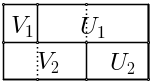
\includegraphics[width=2.4cm,height=1.2cm,scale=0.22]{diagram1.png}\vspace{-4pt}\par\quad
Let $V=\Fbb^3,B_V=\Par{e_1,e_2,e_3},\;V_1=\Span{e_1},\;U_1=\Span{e_2,e_3},\;V_2=\Span{e_1,e_2},\;U_2=\Span{e_3}.$\par\quad
Now $V_1\subseteq V_2,\;U_2\subseteq U_1$ and $V_1\oplus U_1=V_2\oplus U_2.$ But $V_1\neq V_2,\;U_1\neq U_2.$\PfEnd
\SepLine

%\ProblemN{\hypertarget{1C22}{22}}{
%	\TextNL{Suppose $U=\Bra{\Par{x,y,x+y,x-y,2x}\in\Fbb^5}$.}
%	\TextNL{Find nonzero subsps $W_1,W_2,W_3$ of $\,\Fbb^5$ such that $\Fbb^5 = U\oplus W_1\oplus W_2\oplus W_3 $.}
%}\par\quad
%(1) Let $W_1=\Bra{\Par{0,0,z,0,0}\in\Fbb^5}\Rightarrow W_1\cap U=\zeroSubs.$ Now $U\oplus W_1=\Bra{\Par{x,y,z,x-y,2x}\in\Fbb^5}=U_1$.\par\quad
%(2) Let $W_2=\Bra{\Par{0,0,0,w,0}\in\Fbb^5}\Rightarrow W_2\cap U_1=\zeroSubs.$ Now $U_1\oplus W_2=\Bra{\Par{x,y,z,w,2x}\in\Fbb^5}=U_2$.\par\quad
%(3) Let $W_3=\Bra{\Par{0,0,0,0,u}\in\Fbb^5}\Rightarrow W_3\cap U_2=\zeroSubs.$ Now $U_2\oplus W_3=\Bra{\Par{x,y,z,w,u}\in\Fbb^5}=U_3$.\par\quad
%Thus $\Fbb^5=\BigPar{\Par{U\oplus W_1}\oplus W_2}\oplus W_3.$\PfEnd
%\SepLine

\ProblemN{\hypertarget{1C24}{24}}{
	\TextNL{Let $V_E=\Bra{\,f\in\Rbb^{\Rbb}:\text{f is even}},V_O=\Bra{\,f\in\Rbb^{\Rbb}:\text{f is odd}}.$ Show that $V_E\oplus V_O=\Rbb^{\Rbb}.$\vspace{4pt}}
}(a) {$V_E\cap V_O=\Bra{\,f\in\Rbb^{\Rbb}:f\Par{x}=f\Par{-x}=-f\Par{-x}}=\zeroSubs.$}\par\vspace{8pt}
\Blind{\Solution} (b) $\hMath{l}{\left|}{\right\}}{$
	Let $f_e\Par{x}=\Frac{1}{2}\Sbra{g\Par{x}+g\Par{-x}}\Longrightarrow f_e\in V_E\vspace{4pt}\\$
	Let $f_o\Par{x}=\Frac{1}{2}\Sbra{g\Par{x}-g\Par{-x}}\Longrightarrow f_o\in V_O
	}\Rightarrow\forall g\in\Rbb^\Rbb,g\Par{x}=f_e\Par{x}+f_o\Par{x}.$\PfEnd
\SepLine
\ChEnd

\vfill\ChDecl{Ch2A}{2$\cdot$A}{}\orMode{\hLk{2A1}{1}\;\;\hLk{2A2}{2}\;\;\hLk{2A6}{6}\;\;\hLk{2A10}{10}\;\;\hLk{2A11}{11}\;\;\hLk{2A14}{14}\;\;\hLk{2A16}{16}\;\;\hLk{2A17}{17}\;\;|\;\;\hLk{2A4e314}{4E: 3,14}}{[1]: 2; [2]: 1, 6, (4E 3, 14), 10; [3]: 11, 14, 16, 17.}

\ProblemN{\hypertarget{2A2}{2}}{
	(a) \TextN{[P]\hspace{17pt}{\; A list $\Par{v}$ of length $1$ in $V$ is linely inde $\Longleftrightarrow v\neq 0.$} \hfill[Q]}
	(b) \TextN{[P]{\; A list $\Par{v,w}$ of length $2$ in $V$ is linely inde $\Longleftrightarrow\forall\lambda,\mu\in\Fbb,v\neq \lambda w,w\neq \mu v.$} \hfill[Q]}
}\par\quad
(a) $Q\overset{1}{\Rightarrow} P:$ $v\neq 0\Rightarrow$ if $av=0$ then $a=0\Rightarrow\Par{v}$ linely inde.\par\quad\Ha
$P\overset{2}{\Rightarrow} Q:$ $\Par{v}$ linely inde $\Rightarrow v\neq 0$, for if $v=0,$ then $av=0\notRightarrow a=0.$\par\vspace{2pt}\quad\Ha
\Or $\MathLeftMid{l}{{}^\neg Q\overset{3}{\Rightarrow}{}^\neg P:$ $v=0\Rightarrow av=0$ while we can let $a\neq 0\Rightarrow\Par{v}$ is linely dep.$\\ {}^\neg P\overset{4}{\Rightarrow}{}^\neg Q:$ $\Par{v}$ linely dep $\Rightarrow av=0$ while $a\neq 0\Rightarrow v=0.$
$}$\par\vspace{4pt}\quad\Ha
\Comment\,\,\, (1) with (3) and (2) with (4) will do as well.\PfEnd\vspace{6pt}\quad
(b) $P\overset{1}{\Rightarrow}Q:$ $\Par{v,w}$ linely inde $\Rightarrow$  if $av+bw=0,$ then $a=b=0\Rightarrow$ no scalar multi.\par\quad\Hb
$Q\overset{2}{\Rightarrow} P:$ no scalar multi $\Rightarrow$ if $av+bw=0,$ then $a=b=0\Rightarrow\Par{v,w}$ linely inde.\par\vspace{2pt}\quad\Hb
\Or $\MathLeftMid{l}{{}^\neg P\overset{3}{\Rightarrow}{}^\neg Q:$ $\Par{v,w}$ linely dep $\Rightarrow$ if $av+bw=0,$ then $a$ or $b\neq 0\Rightarrow$ scalar multi $\\{}^\neg Q\overset{4}{\Rightarrow}{}^\neg P:$ scalar multi $\Rightarrow$ if $av+bw=0,$ then $a$ or $b\neq 0\Rightarrow$ linely dep. $}$
\par\vspace{4pt}\quad\Hb
\Comment\,\,\, (1) with (3) and (2) with (4) will do as well.\PfEnd
\SepLine\pagebreak

\ProblemN{\hypertarget{2A1}{1}}{
	\TextN{Prove that [P] $\Par{v_1,v_2,v_3,v_4}$ spans $V\Longleftrightarrow\Par{v_1-v_2,v_2-v_3,v_3-v_4,v_4}$ also spans V [Q].}
}\par\quad
Notice that $V=\Span{v_1,\dots,v_n}\Longleftrightarrow\forall v\in V,\exists\,a_1,\dots,a_n\in\Fbb,v=a_1v_1+\dots+a_nv_n.$\par\quad
Assume that $\forall v\in V,\exists\,a_1,\dots,a_4,b_1,\dots,b_4\in\Fbb,$ ( that is, if $\exists\,a_i,$ then we are to find $b_i,$ vice versa )$\\[-6pt] $
\AlignEq{}{v&=a_1 v_1+a_2 v_2+a_3 v_3+a_4 v_4\\[-2pt]&=b_1\Par{v_1-v_2}+b_2\Par{v_2-v_3}+b_3\Par{v_3-v_4}+b_4 v_4\\[-2pt]&=b_1 v_1+\Par{b_2-b_1}v_2+\Par{b_3-b_2}v_3+\Par{b_4-b_3}v_4.\hspace{88pt}}\vspace{-3pt}\par\quad
Now we can let $b_i=\sum_{r=1}^i a_r$ if we are to prove $Q$ with $P$ already assumed;\par\quad
\Blind{Now we can} or let $a_i=b_i-b_{i-1}$ with $b_{0}=0,$ if we are to prove $P$ with $Q$ already assumed.\PfEnd
\SepLine

\ProblemN{\hypertarget{2A6}{6}}{
	\TextN{Prove that [P] $\Par{v_1,v_2,v_3,v_4}$ is linely inde}
	\TextN{\Blind{Prove that} $\Longleftrightarrow\Par{v_1-v_2,v_2-v_3,v_3-v_4,v_4}$ is linely inde. [Q]\vspace{-6pt}}
}\vspace{10pt}\AlignEq{}{P\Rightarrow Q:\;&a_1\Par{v_1-v_2}+a_2\Par{v_2-v_3}+a_3\Par{v_3-v_4}+a_4 v_4=0\\[-2pt]\Rightarrow\;&a_1 v_1+\Par{a_2-a_1}v_2+\Par{a_3-a_2}v_3+\Par{a_4-a_3}v_4=0\Rightarrow a_1=a_2-a_1=a_3-a_2=a_4-a_3=0\\Q\Rightarrow P:\;&a_1 v_1+a_2 v_2+a_3 v_3+a_4 v_4=0\\[-2pt]\Rightarrow\;&a_1\Par{v_1-v_2}+\Par{a_1+a_2}\Par{v_2-v_3}+\Par{a_1+a_2+a_3}\Par{v_3-v_4}+\Par{a_1+\dots+a_4}v_4=0\\[-2pt]\Rightarrow\;&a_1=a_1+a_2=a_1+a_2+a_3=a_1+\dots+a_4=0.}\PfEnd[-30pt]
\SepLine

\ProblemB{
	\hypertarget{2A4e314}{}\TextB{Suppose $\Par{v_1,\dots,v_m}$ is a list of vecs in $V$. For each $k$, let $w_k=v_1+\dots+v_k$.}
	(a) \TextB{Show that $\Span{v_1,\dots,v_m}=\Span{w_1,\dots,w_m}.$}
	(b) \TextB{Show that [P] $\Par{v_1,\dots,v_m}$ is linely inde $\Longleftrightarrow$ $\Par{w_1,\dots,w_m}$ is linely inde [Q].}
}\par\quad
(a) Assume $a_1v_1+\dots+a_mv_m=b_1w_1+\dots+b_mw_m=b_1v_1+\dots+b_k\Par{v_1+\dots+v_k}+\dots+b_m\Par{v_1+\dots+v_m}.$\par\quad\Ha
Then $a_k=b_k+\dots+b_m;\;\;a_{k+1}=b_{k+1}+\dots+b_m\Rightarrow b_k=a_k-a_{k+1};\;b_m=a_m.$ Similar to Problem (1).\vspace{2pt}\par\quad
(b) $P\Rightarrow Q:\;\;b_1 w_1+\dots+b_m w_m=0=a_1 v_1+\dots+a_m v_m,\text{\;where\;}0=a_k=b_k+\dots+b_m.$\par\quad\Hb
$Q\Rightarrow P:\;\;a_1 v_1+\dots+a_m v_m=0=b_1 w_1+\dots+b_m w_m=0, \text{\;where\;} 0=b_m=a_m,\;0=b_k=a_k-a_{k+1}.$\vspace{4pt}\par\quad\Hb
\Or Because $W=\Span{v_1,\dots,v_m}=\Span{w_1,\dots,w_m}.$\par\quad\Hb
By [2.21](b), a list of length $\Par{m-1}$ spans $W,$ then by [2.23],\par\quad\Hb
$\Par{w_1,\dots,w_m}$ linely dep $\Longrightarrow\Par{v_1,\dots,v_m}$ linely dep. Conversely it is true as well.\PfEnd
\SepLine

\ProblemN{\hypertarget{2A10}{10}}{
	\TextNL{Suppose $\Par{v_1,\dots,v_m}$ is linely inde in $V$ and $w\in V$.}
	\TextNL{Prove that if $\Par{v_1+w,\dots,v_m+w}$ is linely depe, then $w\in\Span{v_1,\dots,v_m}$.}
}\par\quad
Suppose $a_1\Par{v_1+w}+\dots+a_m\Par{v_m+w}=0,\exists\,a_i\neq 0\Rightarrow a_1 v_1+\dots+a_m v_m=-\Par{a_1+\dots+a_m}w.$\par\quad
Then $a_1+\dots+a_m\neq 0$, for if not, $a_1 v_1+\dots+a_m v_m=0$ while $a_i\neq 0$ for some $i$, contradicts.%\par\quad Hence $w\in\Span{v_1,\dots,v_m}.$
\PfEnd\vspace{2pt}\quad
\Or By contrapositive: Prove that $w\not\in\Span{v_1,\dots,v_m}\Longrightarrow\Par{v_1+w,\dots,v_m+w}$ is linely inde.\par\quad
Suppose $a_1\Par{v_1+w}+\dots+a_m\Par{v_m+w}=0\Rightarrow a_1v_1+\dots+a_mv_m=-\Par{a_1+\dots+a_m}w.$\par\quad
Now by assumption, $a_1+\dots+a_m=0.$ Then $a_1v_1+\dots+a_mv_m=0\Rightarrow a_1=\dots=a_m=0.$\PfEnd\vspace{2pt}\quad
\Or $\exists\,j\in\!\Bra{1,\dots,m},v_j+w\in\Span{v_1+w,\dots,v_{j-1}+w}.$ If $j=1$ then $v_1+w=0$ and we are done.\par\quad
If $j\geqslant 2,$ then $\exists\,a_i\in\Fbb,v_j+w=a_1\Par{v_1+w}+\dots+a_{j-1}\Par{v_{j-1}+w}\Longleftrightarrow v_j+\lambda w=a_1 v_1+\dots+a_{j-1}v_{j-1}.$\par\quad
Where $\lambda=1-\Par{a_1+\dots+a_{j-1}}.$ Note that $\lambda\neq 0,$ for if not, $v_j+\lambda w=v_j\in\Span{v_1,\dots,v_{j-1}},$ contradicts.\par\quad
Now $w=\lambda^{-1}\Par{a_1 v_1+\dots+a_{j-1}v_{j-1}-v_j}\Rightarrow w\in\Span{v_1,\dots,v_m}.$\PfEnd
\SepLine

\ProblemN{\hypertarget{2A11}{11}}{
	\TextNL{Suppose $\Par{v_1,\dots,v_m}$ is linely inde in $V$ and $w\in V$.}
	\TextNL{Show that [P] $\Par{v_1,\dots,v_m,w}$ is linely inde $\Longleftrightarrow w\not\in\Span{v_1,\dots,v_m}$ [Q].\vspace{8pt}}
}\hspace{-7pt}$\begin{array}{l}{}^\neg Q\Rightarrow{}^\neg P:$ Suppose $w\in\Span{v_1,\dots,v_m}$. Then $\Par{v_1,\dots,v_m,w}$ is linely depe.$\\{}^\neg P\Rightarrow{}^\neg Q:$ Suppose $\Par{v_1,\dots,v_m,w}$ is linely dep. Then by [2.21](a), $w\in\Span{v_1,\dots,v_m}.\end{array}$\PfEnd[-13pt]\vspace{-4pt}
\SepLine

\ProblemN{\hypertarget{2A14}{14}}{
	\TextNL{Prove that [P] $V$ is infinite-dim $\Longleftrightarrow[Q]\left|\hspace{-6pt}\begin{array}{l}$ there is a sequence $\Par{v_1,v_2,\dots}$ in $V$ such that$\\[-8pt]$ $\Par{v_1,\dots,v_m}$ is linely inde for each $m\in\Nbp.\end{array}\right.$}
}\par\quad
$P\Rightarrow Q:\;$ Suppose $V$ is infinite-dim, so that no list spans $V$.\par\quad
\Blind{$P\Rightarrow Q:\;$} {\tgbf Step 1}\;\; Pick a $v_1\neq 0,\Par{v_1}$ linely inde.\par\quad
\Blind{$P\Rightarrow Q:\;$} {\tgbf Step m}\; Pick a $v_m\not\in\Span{v_1,\dots,v_{m-1}},$ by Problem (11), $\Par{v_1,\dots,v_m}$ is linely inde.\par\quad
\Blind{$P\Rightarrow Q:\;$} This process recursively defines the desired sequence $\Par{v_1,v_2,\dots}.$\vspace{4pt}\par\quad
${}^\neg P\Rightarrow{}^\neg Q:\;$ Suppose $V$ is finite-dim and $V=\Span{w_1 , ..., w_m}$.\par\quad
\Blind{${}^\neg P\Rightarrow{}^\neg Q:\;$} Let $\Par{v_1 , v_2 , \dots}$ be a sequence in $V$, then $\Par{v_1,v_2,\dots,v_{m+1}}$ must be linely dep.\vspace{4pt}\par\quad
\Or\; $Q\Rightarrow P:\;$ Suppose there is such a sequence.\par\quad
\Blind{\Or\; $Q\Rightarrow P:\;$} Choose an $m$. Suppose a linely inde list $\Par{v_1,\dots,v_m}$ spans $V$.\par\quad
\Blind{\Or\; $Q\Rightarrow P:\;$} Similar to [2.16]. $\exists\,v_{m+1}\in V\backslash\Span{v_1,\dots,v_m}.$ Hence no list spans $V.$\PfEnd
\SepLine

%\ProblemN{15}{
%	\TextNL{Prove that $\Fbb^\infty$ is infinite-dim.}
%}\par\quad
%Let $e_i=(0,\dots,0,1,0,\dots)\in\Fbb^\infty$ for every $m\in\Nbp$, where $‘1’$ is on the $i^\text{th}$ entry of $e_i$.\par\quad
%Suppose $\Fbb^\infty$ is finite-dim and $\Span{e_1,\dots,e_m}=V$. But $\exists\,e_{m+1}\not\in\Span{e_1,\dots,e_m}$. Contradicts. \PfEnd
%\SepLine

\ProblemN{\hypertarget{2A16}{16}}{
	\TextNL{Prove that the vecsp of all continuous functions in $\Rbb^{[0,1]}$ is infinite-dim.}
}Denote the vecsp by $U$.\par\quad
Choose one $m\in\Nbp.$ Suppose $a_0,\dots,a_m\in\Rbb$ are such that $p\Par{x}=a_0+a_1 x+\dots+a_m x^m=0,\,\forall x\in\Sbra{0,1}.$\par\quad
Then $p$ has infinitely many roots and hence each $a_k=0,$ otherwise $\deg p\geqslant 0,$ contradicts [4.12].\par\quad
Thus $\Par{1,x,\dots,x^m}$ is linely inde in $\Rbb^{[0,1]}.$ Similar to [2.16], $U$ is infinite-dim.\PfEnd\vspace{10pt}\quad
\Or Note that\; $\Frac{1}{1}>\Frac{1}{2}>\dots>\Frac{1}{m},\,\,\,\forall m\in\Nbp.$ Suppose\; $f_m=\left\{\begin{array}{l}
	\hspace{-4pt}x-{\Frac{1}{m}},\;\;x\in\XInterval{(}{]}{\;\Frac{1}{m},\;1\;}\\
	\hspace{-4pt}0,\hfill x\in\XSbra{\;0,\;\Frac{1}{m}\;}\end{array}\right.$\vspace{4pt}\par\quad
Then\; $f_1\XPar{\Frac{1}{m}}=\dots=f_m\XPar{\Frac{1}{m}}=0\neq f_{m+1}\XPar{\Frac{1}{m}}.$ 
Hence $f_{m+1}\not\in\Span{f_1,\dots,f_m}.$ By Problem (14).\PfEnd
\SepLine

\ProblemN{\hypertarget{2A17}{17}}{
	\TextNL{Suppose $p_0,p_1,\dots,p_m\in\PoF{m}$ such that $p_k\Par{2}=0$ for each $k\in\!\Bra{0,\dots,m}$.}
	\TextNL{Prove that $\Par{p_0,p_1,\dots,p_m}$ is not linely inde in $\PoF{m}$.}
}\par\quad
Suppose $\Par{p_0,p_1,\dots,p_m}$ is linely inde. Define $p\in\PoF{m}$ by $p\Par{z}=z.$\par\quad
\NOTICE that $\forall a_i\in\Fbb,z\neq a_0 p_0\Par{z}+\dots+a_m p_m\Par{z},$ for if not, let $z=2.$ Thus $z\not\in\Span{p_0,p_1,\dots,p_m}$.\par\quad
Then $\Span{p_0,p_1,\dots,p_m}\subsetneq\PoF{m}$ while the list $\Par{p_0,p_1,\dots,p_m}$ has length $\Par{m+1}$.\par\quad
Hence $\Par{p_0,p_1,\dots,p_m}$ is linely depe in $\PoF{m}$.\par\quad
For if not, then because $\Par{1,z,\dots,z^m}$ of length $\Par{m+1}$ spans $\PoF{m},$\par\quad
by the steps in [2.23] trivially, $\Par{p_0,p_1,\dots,p_m}$ of length $\Par{m+1}$ spans $\PoF{m}.$ Contradicts.\PfEnd\vspace{10pt}\par\quad
\Or Note that $\PoF{m}=\Span{\underbrace{\;1,\;z,\;\dots,\;z^m\;}_{\text{of length }\Par{m+1}}}.$ Then $\Par{p_0,p_1,\dots,p_m,z}$ of length $\Par{m+2}$ is linely dep.\vspace{3pt}\par\quad
As shown above,  $z\not\in\Span{p_0,p_1,\dots,p_m}.$ And hence $\Par{p_0,p_1,\dots,p_m}$ is linely dep.\PfEnd
\SepLine
\ChEnd\pagebreak

\ChDecl{Ch2B}{2$\cdot$B}{}\orMode{\hLk{2B1}{1}\;\;\hLk{2B7}{7}\;\;\hLk{2B8}{8}\;\;|\;\;\hLk{2B4e5}{4E: 5,}\;\;\hLk{2B4e9}{\!9}}{[1]: 7, 1, (4E 9,5), 8.}
\vspace{8pt}

\ProblemN{\hypertarget{2B7}{7}}{
	\TextN{Prove or give a counterexample\hspace{1pt}$:$ If $\Par{v_1,v_2,v_3,v_4}$ is a basis of \,$V$ and $U$ is a subsp of \,$V$}
	\TextN{such that $v_1,v_2\in U$ and $v_3\not\in U$ and $v_4\not\in U$, then $\Par{v_1,v_2}$ is a basis of U.}
}A counterexample\hspace{1pt}$:$\par\quad
Let $V=\Rbb^4$ and $e_j$ be the $j^\text{th}$ standard basis.\par\quad
Let $v_1=e_1,v_2=e_2,v_3=e_3+e_4,v_4=e_4.$ Then $\Par{v_1,\dots,v_4}$ is a basis of $\Rbb^4.$\par\quad
Let $U=\Span{e_1,e_2,e_3}=\Span{v_1,v_2,v_3-v_4}.$ Then $v_3\not\in U$ and $\Par{v_1,v_2}$ is not a basis of $U.$\PfEnd\SepLine

\BulletPointX\NoteForSmall{\Large $“\complement_V U \cup \zeroSubs”$}\TextB{}
$“\complement_V U \cup \zeroSubs”$ is supposed to be a subsp $W$ such that $V=U\oplus W$.\TextB{}
But if we let $u\in U\backslash\zeroSubs$ and $w\in W\backslash\zeroSubs$, then $\MathRightBrace{l}{w\in\complement_V U \cup \zeroSubs\\ u\pm w\in\complement_V U \cup \zeroSubs }\Rightarrow u\in\complement_V U \cup \zeroSubs.$ Contradicts.\vspace{4pt}\TextB{}
To fix this, {\Large\envFontLarge denote the set $\Bra{W_1,W_2\dots}$ by $\mathcal{S}_V U$,} {\small where for each $W_i,V=U\oplus W_i$. See also in (1.C.23).}\par\SepLine

\ProblemN{\hypertarget{2B1}{1}}{
	\TextN{Find all vecsps that have exactly one basis.}
}The trivial vecsp $\zeroSubs$ will do. Indeed, the only basis of $\zeroSubs$ is the empty list.\par\quad
Now consider a field containing only the add identity $0$ and the multi identity $1$,\par\quad
and we specify that $1+1=0.$ Hence the vecsp $\Bra{0,1}$ will do, the list $\Par{1}$ will be the unique basis.\par\quad
And more generally, consider $\Fbb=\Zbb_m,\forall m-1\in\Nbp.$ For each $s,t\in\Bra{1,\dots,m},$\par\quad
$\Fbb=\Span{K_s}=\Span{K_t}.$ Hence we fail.
Are there other vecsps? Suppose so.\par\quad
(I) Consider $\Fbb=\Rbb$ or $\Cbb$. Let $\Par{v_1,\dots,v_m}$ be a basis of $V\neq\zeroSubs$.\par\quad\HI
While there are infinitely many bases distinct from this one. Hence we fail.\par\quad\EndI
(II) Consider other $\Fbb.$ Note that a field contains at least $0$ and $1$\par\quad\HII
By {\tgsc some theories or facts} given in the course of Elementary Abstract Algebra, we fail.\PfEnd
\SepLine

\ProblemB{
	\hypertarget{2B4e9}{}\TextB{Suppose $\Par{v_1,\dots,v_m}$ is a list of vecs in $V$. For $k\in\Bra{1,\dots,m}$, let $w_k=v_1+\dots+v_k.$}
	\TextB{Show that [P] $B_V=\Par{v_1,\dots,v_m}\Longleftrightarrow B_W=\Par{w_1,\dots,w_m}.$ [Q]}
}\NOTICE that $B_U=\Par{u_1,\dots,u_n}\Longleftrightarrow\forall u\in U,\exists\,!\,a_i\in\Fbb,u=a_1 u_1+\dots+a_n u_n.$\par\quad
$P\Rightarrow Q:\forall v\in V,\exists\,!\,a_i\in\Fbb,\;v=a_1 v_1+\dots+a_m v_m\Rightarrow v=b_1 w_1+\dots+b_m v_m,\exists\,!\,b_k=a_k-a_{k+1},b_m=a_m.$\vspace{2pt}\par\quad
$Q\Rightarrow P:\forall v\in V,\exists\,!\,b_i\in\Fbb,\;v=b_1w_1+\dots+b_mw_m\Rightarrow v=a_1v_1+\dots+a_mv_m,\exists\,!\,a_k=\sum_{j=k}^m b_j.$\PfEnd
\SepLine

\ProblemB{
	\hypertarget{2B4e5}{}\TextB{Suppose $U,W$ are finite-dim and $V=U+W.$ Let $B_U=\Par{u_1,\dots,u_m},\;B_W=\Par{w_1,\dots,w_n}.$}
	\TextB{Prove that $\exists\,B_V$ consisting of vecs in $U\cup W$.}
}Because $V=\Span{u_1,\dots,u_m}+\Span{w_1,\dots,w_n}=\Span{u_1,\dots,u_m,w_1,\dots,w_n}.$\par
\Blind{\Solution} By [2.10], $V$ is finite-dim. By [2.31], $B_V=\Par{u_1,\dots,u_m,w_1,\dots,w_n}.$\PfEnd
\SepLine

\ProblemN{\hypertarget{2B8}{8}}{
	\TextN{Suppose $V=U\oplus W.$ Let $B_U=\Par{u_1,\dots,u_m},\;B_W=\Par{w_1,\dots,w_n}.$}
	\TextN{Prove that $B_V=\Par{u_1,\dots,u_m,w_1,\dots,w_n}$.}
}\par\quad
$\forall v\in V,\exists\,!\,u\in U,w\in W\Rightarrow\exists\,!\,a_i,b_i\in\Fbb,v=u+w=\Par{a_1 u_1+\dots+a_m u_m}+\Par{b_1 w_1+\dots+b_n w_n}.$\PfEnd\quad
\Or\;$V=\Span{u_1,\dots,u_m}\oplus\Span{w_1,\dots,w_n}=\Span{u_1,\dots,u_m,w_1,\dots,w_n}.$\vspace{2pt}\par\quad
\Blind{\Or\;}Note that $\sum_{i=1}^ma_iu_i+\sum_{i=1}^nb_iw_i=0\Rightarrow\sum_{i=1}^ma_iu_i=-\sum_{i=1}^nb_iw_i\in U\cap W=\zeroSubs.$\PfEnd
\SepLine

\BulletPointX\NoteFor{\tgsl linely inde sequence and [2.34]}\TextB{}
$“V=\Span{v_1,\dots,v_n,\dots}”$ is an invalid expression.\TextB{}
If we allow using $“$infinite list$”$, then we must guarantee that $\Par{v_1,\dots,v_n,\dots}$ is a spanning $“$list$”$\TextB{}
such that for all $v\in V$, there exists a smallest positive integer $n$ such that $v=a_1 v_1+\dots+a_n v_n$,\TextB{}
The key point is, how can we guarantee that such a $“$list$”$ exists?\TextB{}
\colorbox{yellow}{TODO: More details.}\TextB{}
\TextB{}
\SepLine\ChEnd

\ChDecl{Ch2C}{2$\cdot$C}{}\orMode{\hLk{2C1}{1}\;\;\hLk{2C7}{7}\;\;\hLk{2C9}{9}\;\;\hLk{2C10}{10}\;\;\hLk{2C14}{14,\,16}\;\;\hLk{2C15}{15}\;\;\hLk{2C17}{17}\;\;|\;\;\hLk{2C4e10}{4E: 10,}\;\;\hLk{2C4e14}{14,}\;\;\hLk{2C4e15}{15,}\;\;\hLk{2C4e16}{16}}{[1]: 7, 9, (4E 16); [2]: 10; [3]: (4E 10), 1; [4]: 14, 17; [5]: (4E 14, 15), 15.}

\vspace{8pt}

\ProblemN{\hypertarget{2C7}{7}}{
	(a) \TextN{Let $U=\Bra{p\in\PoF{4}:p\Par{2}=p\Par{5}=p\Par{6}}$. Find a basis of $U$.}
	(b) \TextN{Extend the basis in {\tgnr(b)} to a basis of $\PoF{4}$.}
	(c) \TextN{Find a subsp $W$ of $\PoF{4}$ such that $\PoF{4}=U\oplus W$.}
}
%Suppose $p\Par{z}=az^4+bz^3+cz^2+dz+e$ such that $p\Par{2}=p\Par{5}=p\Par{6}$.\vspace{4pt}\par\quad
%Then $\hMath[0pt]{r}{\left|}{\right\}}{
	%	p\Par{2}=16a+8b+4c+2d+e\,\;\;\Par{\text{I}}\;\;\\
	%	p\Par{5}=625a+125b+25c+5d+e\;\;\Par{\text{II}}\,\;\\
	%	p\Par{6}=1296a+216b+36c+6d+e\;\,\Par{\text{III}}
	%}\Rightarrow\MathLeftBrace{l}{
	%	\Par{\text{II}}\;-\;\Par{\text{I}}=0\\
	%	\Par{\text{III}}-\Par{\text{II}}=0\\
	%	\Par{\text{III}}-\;\Par{\text{I}}=0\\
	%}$\vspace{4pt}\par\quad
%{\tgsl You don't have to compute to know that the dimension of the set of solutions is 3.}\par\quad
\NOTICE that $\not\exists\,p\in\PoF{}$ of deg $1$ and $2,\;p\in U.$ Thus $\dim U\leqslant \dim\PoF{4}-2=3.$\par\quad
(a) Consider $B=\BigPar{1,\Par{z-2}\Par{z-5}\Par{z-6},z\Par{z-2}\Par{z-5}\Par{z-6}}.$\par\quad\Ha
Because $a_0+a_3\Par{z-2}\Par{z-5}\Par{z-6}+a_4z\Par{z-2}\Par{z-5}\Par{z-6}=0\Rightarrow a_0=a_3=a_4.$\par\quad\Ha
The list $B$ is linely inde in $U.$ Now $\dim U\geqslant 3\Rightarrow \dim U=3.$ Thus $B_U=B.$\par\quad
(b) Extend to a basis of $\PoF{4}$ as $\BigPar{1,z,z^2,\Par{z-2}\Par{z-5}\Par{z-6},z\Par{z-2}\Par{z-5}\Par{z-6}}.$\par\quad
(c) Let $W=\Span{z,z^2}=\Bra{az+bz^2:a,b\in\Fbb}$, so that $\PoF{4}=U\oplus W.$\PfEnd
\SepLine

\ProblemN{\hypertarget{2C9}{9}}{
		\TextN{Suppose $\Par{v_1,\dots,v_m}$ is linely inde in $V$ and $w\in V$.}
		\TextN{Prove that $\dim\Span{v_1+w,\dots,v_m+w}\geq m-1$.}
}Using the result of Problem (10) and (11) in 2.A.\par\quad
Note that $v_i-v_1=\Par{v_i+w}-\Par{v_1+w}\in\Span{v_1+w,\dots,v_n+w},$ for each $i=1,\dots,m$.\par\quad
$\Par{v_1,\dots,v_m}$ linely inde $\Rightarrow$ $\Par{v_1,v_2-v_1,\dots,v_m-v_1}$ linely inde $\Rightarrow$ $\underbrace{\Par{v_2-v_1,_{}\dots,v_m-v_1}}_{\text{of length }\Par{m-1}}$ linely inde.\vspace{-16pt}\par\quad
又 $w\not\in\Span{v_1,\dots,v_m}\Rightarrow\Par{v_1+w,\dots,v_m+w}$ is linely inde.\par\quad
Hence $m\geqslant\dim\Span{v_1+w,\dots,v_m+w}\geq m-1.$\PfEnd
\SepLine

\ProblemBnoor{\hypertarget{2C4e16}{4E 2.C.16}}{
	\TextB{}
	\TextB{Suppose $V$ is finite-dim and $U$ is a subsp of \,$V$ with $U\neq V$. Let $n=\dim V,m=\dim U$.}
	\TextB{Prove that $\exists\,\Par{n-m}$ subsps  $U_1,\dots,U_{n-m}$, each of dim $\Par{n-1}$, such that $\bigcap\limits_{i=1}^{n-m}U_i=U$.}
}\par\quad
Let $\Par{v_1,\dots,v_m}$ be a basis of $U$, extend to a basis of $V$ as $\Par{v_1,\dots,v_m,u_1,\dots,v_{n-m}}$.\par\quad
Define $U_i=\Span{v_1,\dots,v_m,u_1,\dots,u_{i-1},u_{i+1},\dots,u_{n-m}}$ for each $i$. Then $U\subseteq U_i$ for each $i.$\vspace{4pt}\par\quad
And because $\forall v\in \bigcap\limits_{i=1}^{n-m}U_i,v=v_0+b_1 u_1+\dots+b_{n-m} u_{n-m}\in U_i\Rightarrow b_i=0 \text{\;for\;each\;} i\Rightarrow v\in U.$\par\quad
\vspace{6pt}Hence $\bigcap\limits_{i=1}^{n-m}U_i\subseteq U.$\PfEnd
\Example\,\,\, {Suppose $\dim V=6,\dim U=3$.\par\quad
	$\Par{\overbrace{\underbrace{v_1,v_2,v_3}_\text{Basis of U},v_4,v_5,v_6}^\text{Basis of V}},$ define $\hMath[0pt]{l}{\left|}{\right\}}{$
		$U_1=\Span{v_1,v_2,v_3}\oplus\Span{v_5,v_6}\\ $
		$U_2=\Span{v_1,v_2,v_3}\oplus\Span{v_4,v_6}\\ $
		$U_3=\Span{v_1,v_2,v_3}\oplus\Span{v_4,v_5}$
		$}\Rightarrow\dim U_i=6-1,\,\,i=\underbrace{1,2,3}_{6-3=3}.$}
\PfEnd[-10pt]\vspace{-4pt}
\SepLine\pagebreak

\ProblemN{\hypertarget{2C10}{10}}{
	\TextNL{Suppose $m\in\Nbp,\;p_0,p_1,\dots,p_m\in\PoF{}$ are such that each $p_k$ has degree $k.$}
	\TextNL{Prove that $\Par{p_0,p_1,\dots,p_m}$ is a basis of $\PoF{m}$.}
}{\Large\vspace{4pt}Using mathematical induction on $m$.}\par\quad
(i) \envFontLarge{\Large\vspace{8pt}$k=0,1.$ \;$\deg p_0=0;\;\deg p_1=1\Rightarrow\Span{p_0,p_1}=\Span{1,x}.$}\par\quad\Endi
(ii) {\Large\vspace{4pt}$k\in\Bra{1,\dots,m-1}.$ \;Assume that $\Span{p_0,p_1,\dots,p_k}=\Span{1,x,\dots,x^k}.$}\par\quad\Hii
{\Large\vspace{4pt}Then $\Span{p_0,p_1,\dots,p_k,p_{k+1}}\subseteq\Span{1,x,\dots,x^k,x^{k+1}}$.}\par\quad\Hii
{\Large\vspace{4pt}又 $\deg p_{k+1}=k+1,\;\;p_{k+1}\Par{x}=a_{k+1}x^{k+1}+r_{k+1}\Par{x};\;\;a_{k+1}\neq 0,\;\;\deg r_{k+1}\leqslant k.$}
\par\vspace{2pt}\quad\Hii
{\Large\vspace{4pt}$\Rightarrow x^{k+1}=\Frac{1}{a_{k+1}}\XPar{p_{k+1}\Par{x}-r_{k+1}\Par{x}}\in\Span{1,x,\dots,x^k,p_{k+1}}=\Span{p_0,p_1,\dots,p_k,p_{k+1}}$.}\par\vspace{2pt}\quad\Hii
{\Large\vspace{8pt}$\therefore\,\,x^{k+1}\in\Span{p_0,p_1,\dots,p_k,p_{k+1}}\Rightarrow\Span{1,x,\dots,x^k,x^{k+1}}\subseteq\Span{p_0,p_1,\dots,p_k,p_{k+1}}$.}\par\quad
{\Large\vspace{4pt}Thus $\PoF{m}=\Span{1,x,\dots,x^m}=\Span{p_0,p_1,\dots,p_m}.$}\PfEnd\vspace{12pt}\quad
\Or 用比较系数法. {\Large\vspace{4pt}Denote the coefficient of $x^k$ in $p\in\PoF{}$ by $\xi_k\Par{p}.$}\par\quad
{\Large\vspace{4pt}Suppose $L=a_m p_m\Par{x}+\dots+a_1 p_1\Par{x}+a_0p_0\Par{x}=0\cdot x^m+\dots+0\cdot x+0\cdot 1=R,\forall x\in\Fbb.$}\par\quad
{\Large\vspace{4pt}We use induction to show that $a_m=\dots=a_0=0.$}\par\quad
(i) {\Large\vspace{4pt}$k=m,$ \;$\xi_{m}\Par{L}=a_{m}\xi_{m}\Par{p_m}=\xi_{m}\Par{R}=0$ 又 $\deg p_m=m,\;\xi_{m}\Par{p_m}\neq 0\Rightarrow a_m=0.$}\par\quad\Hi
{\Large\vspace{8pt}Now $L=a_{m-1}p_{m-1}\Par{x}+\dots+a_0p_0\Par{x}.$}\par\quad\Endi
(ii) {\Large\vspace{4pt}$1\leqslant k\leqslant m,$ \;$\xi_{k}\Par{L}=a_{k}\xi_{k}\Par{p_k}=\xi_{k}\Par{R}=0$ 又 $\deg p_k=k,\;\xi_{k}\Par{p_k}\neq 0\Rightarrow a_k=0.$}\par\quad\Hii
{\Large Now $L=a_{k-1}p_{k-1}\Par{x}+\dots+a_0p_0\Par{x}.$}\PfEnd
\SepLine

\ProblemBnoor{\Tips}[]{
	\TextB{Suppose $m\in\Nbp,\;p_0,p_1,\dots,p_m\in\PoF{m}$ are such that}
	\Blind{\Tips} \TextB{the lowest term of each $p_k$ is of deg $k.$ Prove that $\Par{p_0,p_1,\dots,p_m}$ is a basis of $\PoF{m}.$}
}{\Large Using mathematical induction on $m.$\par}\quad
\envFontLarge{\Large Let each $p_k$ be defined by $p_k\Par{x}=a_{k,k} x^k+\dots+a_{m,k} x^m,$ where $a_{k,k}\neq 0.$\par}\quad
(i) {\Large$k=0,1.$ \;$p_m\Par{x}=a_{m,m}x^m;\;p_{m-1}\Par{x}=a_{m-1,m-1}x^{m-1}+a_{m,m-1}x^m$\par}\quad\Hii
{\Large\Blind{$k=0,1.$} $\Rightarrow\Span{x^m,x^{m-1}}=\Span{p_m,p_{m-1}}.$\par}\vspace{6pt}\quad\Endi
(ii) {\Large$k\in\Bra{1,\dots,m-1}.$ \;Assume that $\Span{x^m,\dots,x^{m-k}}=\Span{p_m,\dots,p_{m-k}}.$}\par\quad\Hii
{\Large Then $\Span{p_m,\dots,p_{m-\SmallPar{k+1}}}\subseteq\Span{x^m,\dots,x^{m-\SmallPar{k+1}}}.$\par}\quad\Hii
{\Large 又 $p_{m-\SmallPar{k+1}}$ has the form $a_{m-\SmallPar{k+1},m-\SmallPar{k+1}}x^{m-\SmallPar{k+1}}+r_{m-\SmallPar{k+1}}\Par{x};\;$\par}\quad\Hii
{\Large\Blind{又} where the lowest term of $r_{m-\SmallPar{k+1}}\in\PoF{m}$ is of deg $\Par{m-k}.$\par}\vspace{6pt}\quad\Hii
{\Large $\Rightarrow x^{m-\SmallPar{k+1}}=\Frac{1}{a_{m-\SmallPar{k+1},m-\SmallPar{k+1}}}\XPar{p_{m-\SmallPar{k+1}}\Par{x}-r_{m-\SmallPar{k+1}}\Par{x}}$\par}\vspace{4pt}\quad\Hii
{\Large \Blind{$\Rightarrow x^{m-\SmallPar{k+1}}$}${}\in\Span{x^m,\dots,x^{m-k},p_{m-\SmallPar{k+1}}}=\Span{p_m,\dots,p_{m-k},p_{m-\SmallPar{k+1}}}.$\par}\vspace{4pt}\quad\Hii
{\Large$\therefore\;x^{m-\SmallPar{k+1}}\in\Span{p_m,\dots,p_{m-k},p_{m-\SmallPar{k+1}}}$\par}\quad\Hii
{\Large \Blind{$\therefore\;$}$\Rightarrow\Span{x^m,\dots,x^{m-k},x^{m-\SmallPar{k+1}}}\subseteq\Span{p_m,\dots,p_{m-k},p_{m-\SmallPar{k+1}}}.$\par}\vspace{6pt}\quad
{\Large Thus $\PoF{m}=\Span{x^m,\dots,x,1}=\Span{p_m,\dots,p_1,p_0}.$}\PfEnd
\SepLine

\ProblemBnoor{\hypertarget{2C4e10}4E 2.C.10}{
	\TextB{Suppose $m$ is a positive integer. For $0\leqslant k\leqslant m$, let $p_k\Par{x}=x^k\Par{1-x}{^{m-k}}$.}
	\TextB{Show that $\Par{p_0,\dots,p_m}$ is a basis of $\PoF{m}$.}
	\TextB{{\large The basis in this exercise leads to what are called Bernstein polys. You can do a web search to learn how}}
	\TextB{{\large Bernstein polys are used to approximate continuous functions on $[0, 1]$.}}
}\par\quad
Note that each $p_k\Par{x}={\sum_{j=0}^{m-k}\mathC_{m-k}^j\Par{-1}{^{j}}\cdot x^{j+k}\cdot 1^j}=\underset{\text{of deg k}}{\uline{\Par{-1}{^0}\cdot x^k\cdot 1^0}}+\underset{\text{of deg m; denote it by }q_k\SmallPar{x}}{\uline{\sum_{j=1}^{m-k}\mathC_{m-k}^j\Par{-1}{^{j}}\cdot x^{j+k}\cdot 1^j}}.$\vspace{-12pt}\par\quad
And, each $q_k\in\Span{x^{k+1},\dots,x^m}.$ Using \TIPS above.\PfEnd\vspace{6pt}\quad
\Or Using induction.\par\quad
(i) $k=0,1.$ \;$p_m\Par{x}=x^m;\;p_{m-1}\Par{x}=x^{m-1}-x^m\Longrightarrow x^{m-1}=p_{m-1}\Par{x}+p_m\Par{x}.$\vspace{2pt}\par\quad\Endi
(ii) $k\in\Bra{2,\dots,m-1}.$ \;Assume that $x^{m-k}=p_{m-k}\Par{x}+a_mx^m+\dots+a_{m-k+1}x^{m-k+1}.$\vspace{2pt}\par\quad\Hii
Note that $x^{m-k-1}=p_{m-k-1}\Par{x}+\sum_{j=1}^{k+1}\mathC_{k+1}^j\Par{-1}{^{j+1}}x^{j+m-k-1}\Longrightarrow\exists\,!\,c_{m-i}=\mathC_{k+1}^{k+1-i}\Par{-1}{^{k-i}}.$ \Par{$\Delta$}\vspace{2pt}\par\quad
Thus each $x^k=b_mp_m\Par{x}+\dots+b_{m-k}p_{m-k}\Par{x},\exists\,!\,b_{m-i}\in\Fbb.$ \quad\Sbra{ \Par{$\Delta$} is the core. }\PfEnd\quad
\Comment \,\,\,Core and context can be inde. Dependence is not a requisite for combination.\vspace{10pt}\par\quad
\Or For any $m,k\in\Nbp$ such that $k\leqslant m.$ Define $p_{k,m}$ by $p_{k,m}\Par{x}=x^k\Par{1-x}^{m-k}.$\par\quad
Define the statement $S\Par{m}$ by $S\Par{m}:\Par{p_{0,m},\dots,p_{m,m}}$ is linely inde ( and therefore is a basis ).\par\quad
We use induction on to show that $S\Par{m}$ holds for all $m\in\Nbp.$\vspace{4pt}\par\quad
(i) $m=1.$ \;Let $a_0\Par{1-x}+a_1x=0,\forall x\in\Fbb.$ \;Then take $x=1,x=0\Rightarrow a_1=a_0=0.$\par\quad\Hi
$m=2.$ \;Let $a_0\Par{1-x}^2+a_1\Par{1-x}x+a_2x^2,\forall x\in\Fbb.$ \;Then $\MathLeftBrace{l}{x=0\Rightarrow a_0+a_1=0;\\x=1\Rightarrow a_2=0;\\x=2\Rightarrow a_0+2a_1=0.}$\par\quad\Endi
(ii) $2\leqslant m.$ \;Assume that $S\Par{m}$ holds.\vspace{2pt}\par\quad\Hii
\envFontLarge{\vspace{6pt}Suppose\; $\sum_{k=0}^{m+2}a_kp_{k,m+2}\Par{x}=\sum_{k=0}^{m+2}a_kx^k\Par{1-x}^{m+2-k}=0,\forall x\in\Fbb.$}\par\quad\Hii
{\vspace{6pt}While {\Large$x=0\Rightarrow a_0=0;\;x=1\Rightarrow a_{m+2}=0.$} Then {\Large$\sum_{k=1}^{m+1}a_kx^k\Par{1-x}^{m+2-k}=0;$}}\par\quad\Hii
{\vspace{6pt}And note that \Large\AlignEq{}{\\[-45pt]&\textstyle\sum_{k=1}^{m+1}a_kx^k\Par{1-x}^{m+2-k}\\={}&x\Par{1-x}\textstyle\sum_{k=1}^{m+1}a_kx^{k-1}\Par{1-x}^{m+1-k}\\={}&x\Par{1-x}\textstyle\sum_{k=0}^{m}a_{k+1}x^{k}\Par{1-x}^{m-k}=x\Par{1-x}\sum_{k=0}^{m}a_{k+1}p_{k,m}\Par{x}.\hspace{-40pt}}}\vspace{4pt}\par\quad\Hii
\envFontDefault{\vspace{4pt}Hence $x\Par{1-x}\sum_{k=0}^{m}a_{k+1}p_{k,m}\Par{x}=0,\forall x\in\Fbb\Rightarrow \sum_{k=0}^{m}a_{k+1}p_{k,m}\Par{x}=0,\forall x\in\Fbb\backslash\Bra{0,1}.$}\par\quad\Hii
{\vspace{4pt}Because $\sum_{k=0}^{m}a_{k+1}p_{k,m}\Par{x}$ has infinitely many zeros. We have $\sum_{k=0}^{m}a_{k+1}p_{k,m}\Par{x}=0,\forall x\in\Fbb.$}\par\quad\Hii
{\vspace{4pt}By assumption, $a_1=\dots=a_m=0,$ while $a_0=a_{m+2}=0,$}\par\quad\Hii
\Blind{By ass}\vspace{4pt}and also $\;a_{m+1}=0$ \BigPar{ because $\sum_{k=0}^{m}a_{k+1}p_{k,m}\Par{x}=a_{m+1}p_{m,m}\Par{x}=a_{m+1}x^m=0,\forall x\in\Fbb.$ }\par\quad\Hii
\vspace{6pt}Thus $\Par{p_{0,m+2},\dots,p_{m+2,m+2}}$ is linely inde and $S\Par{m+2}$ holds.\par\quad
Since $\forall m\in\Nbp,S\Par{m}\Rightarrow S\Par{m+2}.$ We have \;$\hMath[0pt]{r}{\left|}{\right\}}{\forall k\in\Nbb,S\Par{2k+1}\text{ holds}\\\forall k\in\Nbp,S\Par{2k}\text{ holds}}\Rightarrow S\Par{m}$ holds.\PfEnd
\SepLine

\ProblemNnoor[]{\hypertarget{2C1}{1}}{\COROLLARY\;for [2.38,39]}{
	\TextN{Suppose $U$ is a subsp of \,$V$ such that $\dim V=\dim U$. Then $V=U.$}
}\Blind{\IndentN} Let $B_U=\Par{u_1,\dots,u_m}.$ Then $m=\dim V.$ 又 $u_i\in V.$ By [2.39], $B_V=\Par{u_1,\dots,u_m}.$\PfEnd\vspace{-2pt}
\SepLine[-2pt]

\ProblemBnoor[]{}[]{
	\TextB{\tgnr\envFontDefault\large Let $v_1,\dots,v_n\in V$ and $\dim\Span{v_1,\dots,v_n}=n.$ Then $\Par{v_1,\dots,v_n}$ is a basis of $\Span{v_1,\dots,v_n}.$}
	\TextB{\envFontDefault\large Notice that $\Par{v_1,\dots,v_n}$ is a spanning list of $\Span{v_1,\dots,v_n}$ of length $n=\dim\Span{v_1,\dots,v_n}.$\vspace{-2pt}}
}\SepLine[-2pt]

%\colorbox{yellow}{TODO: More Tips.}
%\par\quad
%\par\quad
%\SepLine

\ProblemN{\hypertarget{2C14}{14}}{
	\TextNL{Suppose that $V_1,\dots,V_m$ are finite-dim subsps of \,$V$.}
	\TextNL{Prove that $V_1+\dots+V_m$ is finite-dim and $\dim\!\Par{V_1+\dots+V_m}\leqslant\dim V_1+\dots+\dim V_m$.}
}\par\quad
Choose a basis $ \mathcal{E}_i$ of $V_i\Rightarrow V_1+\dots+V_m=\Span{\mathcal{E}_1\cup\cdots\cup \mathcal{E}_m};\,\,\,\dim V_i=\card \mathcal{E}_i$.\par\quad
Then $\dim\!\Par{V_1+\dots+V_m}=\dim\Span{\mathcal{E}_1\cup\cdots\cup \mathcal{E}_m}$.\par\quad
又 $\dim\Span{\mathcal{E}_1\cup\cdots\cup\mathcal{E}_m}\leqslant\card\Par{\mathcal{E}_1\cup\cdots\cup \mathcal{E}_m}\leqslant\card \mathcal{E}_1+\cdots+\card \mathcal{E}_m$.\par\quad
Thus $\dim\!\Par{V_1+\dots+V_m}\leqslant \dim V_1+\dots+\dim V_m.$\PfEnd\vspace{6pt}
\Comment \,\,\,{\tgsl\Large$\dim\!\Par{V_1+\dots+V_m}=\dim V_1+\dots+\dim V_m\Longleftrightarrow V_1+\dots+V_m$ is a direct sum.}\par
\Blind{\Comment\,\,\,}For each $i$, $\Par{V_1+\dots+V_i}\cap V_{i+1}=\zeroSubs\Longleftrightarrow V_1+\dots+V_m$ is a direct sum\par
\Blind{\Comment\,\,\,}$\Longleftrightarrow\Par{\mathcal{E}_1\cap\dots\cap\mathcal{E}_{k-1}}\cap\mathcal{E}_k=\emptyset$ for each $i$ 又 $\dim\Span{\mathcal{E}_1\cup\dots\cup\mathcal{E}_m}=\card\Par{\mathcal{E}_1\cup\dots\cup\mathcal{E}_m}$\par
\Blind{\Comment\,\,\,}$\Longleftrightarrow\dim\Span{\mathcal{E}_1\cup\dots\cup\mathcal{E}_m}=\card\mathcal{E}_1+\dots+\card\mathcal{E}_m$\par
\Blind{\Comment\,\,\,}$\Longleftrightarrow\dim\!\Par{V_1+\dots+V_m}=\dim V_1+\dots+\dim V_m.$\PfEnd
\SepLine

\ProblemN{\hypertarget{2C17}{17}}{
	\TextNL{Suppose $V_1,V_2,V_3$ are subsps of a finite-dim vecsp, then}
	\TextNL{{\large\envFontDefault$\Dim\Par{V_1+V_2+V_3}=\dim V_1+\dim V_2+\dim V_3$\par\rightline{$-\Dim\Par{V_1\cap V_2}-\Dim\Par{V_1\cap V_3}-\Dim\Par{V_2\cap V_3}+\Dim\Par{V_1\cap V_2\cap V_3}$.\qquad}}}
	\TextNL{Explain why you might think and prove the formula above or give a counterexample.}
}\par\quad
[{\tgsl Similar to}]\; Given three sets $A,B$ and $C$.\par\quad
Because $\cMid{X+Y}=\cMid{X}+\cMid{Y}-\cMid{X\cap Y};\,\,\,\Par{X\cup Y}\cap Z=\Par{X\cap Z}\cup\Par{Y\cap Z}$.\par\quad
Now $\cMid{\Par{A\cup B}\cup C}=\cMid{A\cup B}+\cMid{C}-\cMid{\Par{A\cup B}\cap C}.$\par\quad
And $\cMid{\Par{A\cup B}\cap C}=\cMid{\Par{A\cap C}\cup\Par{B\cap C}}=\cMid{A\cap C}+\cMid{B\cap C}-\cMid{A\cap B\cap C}.$\par\quad
Hence $\cMid{\Par{A\cup B}\cup C}=\cMid{A}+\cMid{B}+\cMid{C}+\cMid{A\cap B\cap C}-\cMid{A\cap B}-\cMid{A\cap C}-\cMid{B\cap C}.$\par\vspace{4pt}\quad
Because $\Par{V_1+V_2}+V_3=V_1+\Par{V_2+V_3}=\Par{V_1+V_3}+V_2.$\vspace{-6pt}\par\quad
\AlignEq{\hspace{10pt}}{\Dim\Par{V_1+V_2+V_3}&=\Dim\Par{V_1+V_2}+\Dim\Par{V_3}-\Dim\BigPar{\Par{V_1+V_2}\cap V_3}\quad(1)\hspace{114pt}\\&=\Dim\Par{V_2+V_3}+\Dim\Par{V_1}-\Dim\BigPar{\Par{V_2+V_3}\cap V_1}\quad(2)\\&=\Dim\Par{V_1+V_3}+\Dim\Par{V_2}-\Dim\BigPar{\Par{V_1+V_3}\cap V_2}\quad(3)}\par\quad
Notice that in general, $\Par{X+Y}\cap Z\neq X\cap Z+Y\cap Z$.\par\quad
For example, $X=\Bra{\Par{x,0}\in\Rbb^2:x\in\Rbb},Y=\Bra{\Par{0,y}\in\Rbb^2:y\in\Rbb},Z=\Bra{\Par{z,z}\in\Rbb^2:z\in\Rbb}.$\vspace{8pt}\par
\BulletPointX\Corollary \,\,\,\Largesl{Suppose $V_1,V_2$ and $V_3$ are finite-dim vecsps, then} {\small $\Frac{\Par{1}+\Par{2}+\Par{3}}{3}:$
}\vspace{-6pt}\par
\AlignEq{\IndentB\,}{\Dim\Par{V_1+V_2+V_3}=\dim &\,V_1+\dim V_2+\dim V_3\\&-\Frac{\Dim\Par{V_1\cap V_2}+\Dim\Par{V_1\cap V_3}+\Dim\Par{V_2\cap V_3}}{3}\\&-\Frac{\Dim\BigPar{\Par{V_1+V_2}\cap V_3}+\Dim\BigPar{\Par{V_1+V_3}\cap V_2}+\Dim\BigPar{\Par{V_2+V_3}\cap V_1}}{3}.}\TextB{}
{\tgsl The formula above may seem strange because the right side does not look like an integer.\PfEnd}\par
\SepLine

\ProblemB[]{
	\TextB{Suppose V is a 10-dim vecsp and $V_1,V_2,V_3$ are subsps of \,$V$ with}
	\hypertarget{2C4e14}{}(a) \TextB{$\dim V_1 = \dim V_2 = \dim V_3 = 7$. Prove that $V_1\cap V_2\cap V_3\neq\zeroSubs$.}
	\Blind{(a)} By \TIPS, $\Dim\Par{V_1\cap V_2\cap V_3}\geq\dim V_1+\dim V_2+\dim V_3\uline{-2\dim V}>0.$\TextB{\vspace{4pt}}
	\hypertarget{2C4e15}{}(b) \TextB{$\dim V_1+\dim V_2+\dim V_3 > 2\dim V$. Prove that $V_1\cap V_2\cap V_3\neq\zeroSubs$.}
	\Blind{(b)} By \TIPS, $\Dim\Par{V_1\cap V_2\cap V_3}\uuline{{}>2\dim V}-\Dim\Par{V_2+V_3}-\Dim\Par{V_1+\Par{V_2\cap V_3}}\geq 0.$\PfEnd\vspace{14pt}
}\SepLine

\BulletPointX\Tips\TextB{}
Because $\dim \Par{V_1\cap V_2\cap V_3}=\dim V_1+\Dim\Par{V_2\cap V_3}-\Dim\BigPar{V_1+\Par{V_2\cap V_3}}.$\TextB{}
And $\Dim\Par{V_2\cap V_3}=\dim V_2+\dim V_3-\Dim\Par{V_2+V_3}.$ We have $\Par{1},$ and $\Par{2},\Par{3}$ similarly.\TextB{}
$\Par{1}\;\Dim\Par{V_1\cap V_2\cap V_3}=\dim V_1+\dim V_2+\dim V_3-\Dim\Par{V_2+V_3}-\Dim\BigPar{V_1+\Par{V_2\cap V_3}}.$\TextB{}
$\Par{2}\;\Dim\Par{V_1\cap V_2\cap V_3}=\dim V_1+\dim V_2+\dim V_3-\Dim\Par{V_1+V_3}-\Dim\BigPar{V_2+\Par{V_1\cap V_3}}.$\TextB{}
$\Par{3}\;\Dim\Par{V_1\cap V_2\cap V_3}=\dim V_1+\dim V_2+\dim V_3-\Dim\Par{V_1+V_2}-\Dim\BigPar{V_3+\Par{V_1\cap V_2}}.$
\SepLine

\ProblemN{\hypertarget{2C15}{15}}{
	\TextNL{Suppose $V$ is finite-dim and $\dim V=n\geqslant 1.$}
	\TextNL{Prove that $\exists$ one-dim subsps $V_1,\dots,V_n$ of $V$ such that $V=V_1\oplus \dots\oplus V_n.$}
}Suppose $B_V=\Par{v_1,\dots,v_n}.$ Define $V_i$ by $V_i=\Span{v_i}$ for each $i\in\!\Bra{1,\dots,n}.$\par
\Blind{\Solution} Then $\forall v\in V,\exists\,!\,a_i\in\Fbb,v=a_1 v_1+\dots+a_n v_n\Rightarrow\exists\,!\,u_i\in V_i,v=u_1+\dots+u_n$\PfEnd
%\Blind{\Solution} \Blind{Then $\forall v\in$}\hspace{3pt}
\SepLine

\ProblemB[]{
	\Corollary \,\,\,\TextB{Suppose $W$ is finite-dim, $\dim W=m$ and \envFontDefault$w\in W\backslash\zeroSubs.$}
	\Blind{\Corollary \,\,\,}\TextB{Prove that $\exists\,B_W=\Par{w_1,\dots,w_m}$ such that $w=w_1+\dots+w_m.$\vspace{4pt}}
By Problem (15), $\exists$ one-dim subsps $W_1,\dots,W_m$ of $W$ such that $W=W_1\oplus\dots\oplus W_m.$\TextB{}
Note that $\dim W_i=\dim\Span{w_i}=1\Rightarrow\forall x_i\in W_i,\exists\,!\,c_i\in\Fbb,x_i=c_i w_i.$\TextB{}
Suppose $w=x_1+\dots+x_m,$ where each $x_i=c_i w_i\in W_i.$ Then $\Par{x_1,\dots,x_m}$ is also a basis of $W.$\PfEnd\TextB{\vspace{6pt}}
\Or Note that $w\neq 0\Rightarrow m\geqslant 1.$ If $m=1$ then let $w_1=w$ and we are done. Suppose $m>1.$\TextB{}
Extend $\Par{w}$ to a basis $\Par{w,w_1,\dots,w_{m-1}}$ of $W.$ Let $w_m=w-w_1-\dots-w_{m-1}.$\TextB{}
又 $\Span{w,w_1,\dots,w_{m-1}}=\Span{w_1,\dots,w_m}.$ Hence $\Par{w_1,\dots,w_m}$ is also a basis of $W.$\PfEnd\vspace{14pt}
}
\SepLine

\ProblemB[]{
	{\NewTheorem \,\,\,}\TextB{Suppose $V$ is finite-dim with $\dim V=n$ and $U$ is a subsp of \,$V$ with $U\neq V.$}
	\Blind{\NewTheorem\,\,\,}\TextB{Prove that $\exists\,B_V=\Par{v_1,\dots,v_n}$ such that each $v_k\not\in U.$}
}\TextB{\vspace{0pt}}
Note that $U\neq V\Rightarrow n\geqslant 1.$ We will construct $B_V$ via the following process.\TextB{}
{\tgbfx Step 1.} $\exists\,v_1\in V\backslash U\Rightarrow v_1\neq 0.$ If $\Span{v_1}=V$ then we stop.\TextB{}
{\tgbfx Step k.} Suppose $\Par{v_1,\dots,v_{k-1}}$ is linely inde in $V,$ each of which belongs to $V\backslash U.$\TextB{}
\Blind{\tgbfx Step k.} Note that $\Span{v_1,\dots,v_{k-1}}\neq V.$ And if $\Span{v_1,\dots,v_{k-1}}\cup U=V,$ then by (1.C.12),\TextB{}
\Blind{\tgbfx Step k.} ( because $\Span{v_1,\dots,v_{k-1}}\not\subseteq U,$ ) $U\subseteq \Span{v_1,\dots,v_{k-1}}\Rightarrow\Span{v_1,\dots,v_{k-1}}=V.$\TextB{}
\Blind{\tgbfx Step k.} Hence because $\Span{v_1,\dots,v_{k-1}}\neq V,$ it must be case that $\Span{v_1,\dots,v_{k-1}}\cup U\neq V.$\TextB{}
\Blind{\tgbfx Step k.} Thus $\exists\,v_k\in V\backslash U$ such that $v_k\not\in\Span{v_1,\dots,v_{k-1}}.$\TextB{}
\Blind{\tgbfx Step k.} By (2.A.11), $\Par{v_1,\dots,v_k}$ is linely inde in $V$. If $\Span{v_1,\dots,v_k}=V,$ then we stop.\TextB{}
Because $V$ is finite-dim, this process will stop after $n$ steps.\PfEnd\vspace{4pt}\TextB{}
\Or If $U=\zeroSubs$ then we are done. Let $\dim U\geqslant 1.$\TextB{}
Let $\Par{u_1,\dots,u_m}$ be a basis of $U.$ Extend to a basis $\Par{u_1,\dots,u_n}$ of $V.$\TextB{}
Then let $B_V=\Par{u_1-u_k,\dots,u_m-u_k,u_{m+1},\dots,u_k,\dots,u_n}.$\PfEnd
\SepLine
\ChEnd\pagebreak

\ChDecl{Ch3A}{3$\cdot$A}{}\orMode{\hLk{3A3}{3}\;\;\hLk{3A4}{4}\;\;\hLk{3A5}{5}\;\;\hLk{3A7}{7}\;\;\hLk{3A8}{8}\;\;\hLk{3A10}{10}\;\;\hLk{3A11}{11}\;\;\hLk{3A12}{12}\;\;\hLk{3A13}{13}\;\;|\;\;\hLk{3A4e10}{4E: 10,}\;\;\hLk{3A4e11}{11,}\;\;\hLk{3A4e17}{17}}{[1]: (4E 1.B.7), 5; [2]: 3, 4, 7, 8, 9, (4E 3.A.10), 10, 11, 12;$\\$[3]: 13, (4E 3.A.17), (4E 3.B.32); [4]: (4E 3.A.11).}

\vspace{3pt}

\BulletPointX\TipsN{1} \,\,\,$T:V\rightarrow W$ is linear $\Longleftrightarrow\MathLeftrightMid{l}{\hspace{-4pt}$
(一) $\forall v,u\in V,T\Par{v+u}=Tv+Tu;\\\hspace{-4pt} $
(二) $\forall v,u\in V,\lambda\in\Fbb,T\Par{\lambda v}=\lambda\Par{Tv}.$
$}\Longleftrightarrow T\Par{v+\lambda u}=Tv+\lambda Tu.$\vspace{-10pt}
\SepLine

\BulletPointX\TipsN{2} \,\,\,$T\in\Lm{V,W}\Longleftrightarrow T\in\Lm{V,\range T}.$
\SepLine

\BulletPointX\TipsN{3} \,\,\,If $U$ is a subsp of $W,$ then $\Bra{T\in\Lm{V,W}:\range T\subseteq U}=\Lm{V,U}.$
\SepLine

\ProblemBnoor{4E 1.B.7}{
	\TextB{Suppose $V\neq\varnothing$ and $W$ is a vecsp. Let $W^V=\Bra{f:V\rightarrow W}.$}
	(a) \TextB{Define a natural add and scalar multi on $W^V.$}
	(b) \TextB{Prove that $W^V$ is a vecsp with these definitions.}
}\par\quad
(a) $W^V\ni f+g: x\rightarrow f\Par{x}+g\Par{y};$ where $f\Par{x}+g\Par{y}$ is the vec add on $W.$\par\quad\Ha
$W^V\ni\lambda f: x\rightarrow\lambda f\Par{x};$ where $\lambda f\Par{x}$ is the scalar multi on $W.$\par\quad
(b) Commutativity: $\Par{f+g}\Par{x}=f\Par{x}+g\Par{x}=g\Par{x}+f\Par{x}=\Par{g+f}\Par{x}.$\par\quad\Hb
Associativity: $\BigPar{\Par{f+g}+h}\Par{x}=\BigPar{{f}\Par{x}+{g}\Par{x}}+{h}\Par{x}$\par\quad\Hb
\Blind{Associativity: $\BigPar{\Par{f+g}+h}\Par{x}$} $={f}\Par{x}+\BigPar{{g}\Par{x}+{h}\Par{x}}=\BigPar{f+\Par{g+h}}\Par{x}.$\par\quad\Hb
Additive Identity: $\Par{f+0}\Par{x}=f\Par{x}+0\Par{x}=f\Par{x}+0=f\Par{x}.$\par\quad\Hb
Additive Inverse: $\Par{f+g}\Par{x}={f}\Par{x}+g\Par{x}=f\Par{x}+\BigPar{-f\Par{x}}=0=0\Par{x}.$\par\quad\Hb
Distributive Properties:\par\qquad\Hb
$\BigPar{a\Par{f+g}}\Par{x}=a\Par{f+g}\Par{x}=a\BigPar{f\Par{x}+g\Par{x}}$\par\qquad\Hb
\Blind{$\BigPar{a\Par{f+g}}\Par{x}=a\Par{f+g}\Par{x}$} $=a\,f\Par{x}+ag\Par{x}=\Par{a\,f}\Par{x}+\Par{ag}\Par{x}=\Par{a\,f+ag}\Par{x}.$\par\qquad\Hb
Similarly, $\BigPar{\Par{a+b}f}\Par{x}=\Par{a\,f+b\,f}\Par{x}.$\par\quad\Hb
So far, we have used the same properties in $W.$\par\quad\Hb
Which means that {\tgsc if $W^V$ is a vecsp, then $W$ must be a vecsp.}\par\quad\Hb
Multiplication Identity: $\Par{1f}\Par{x}=1f\Par{x}=f\Par{x}.$ \BigPar{ \NOTICE that the smallest $\Fbb$ is $\Bra{0,1}.$ }\PfEnd
\SepLine

\ProblemN[]{\hypertarget{3A5}{5}}{
	\TextN{Because $\Lm{V,W}=\Bra{T:V\rightarrow W\;\mmid\;T\text{ is linear}}$ is a subsp of $W^V,$ $\Lm{V,W}$ is a vecsp.}
}
\SepLine

\ProblemN{\hypertarget{3A3}{3}}{
	\TextN{Suppose $T\in\Lm{\Fbb^n,\Fbb^m}$. Prove that $\exists\,A_{j,k}\in\Fbb\,$such that for any $\Par{x_1,\dots,x_n}\in\Fbb^n,$}\hspace{-40pt}
	\TextN{\centerline{ $T\Par{x_1,\dots,x_n}=\MathLeftrightPare{l}{
	A_{1,1}x_1+\dots+A_{1,n}x_n,\\
	\Blind{A}\!\vdots\Blind{_{1}x_1+}\,\ddots\Blind{+A}\vdots\\
	A_{m,1}x_1+\dots+A_{m,n}x_n}$}}
}\par\quad
Let $T\Par{1,0,0,\dots,0,0}=\Par{A_{1,1},\dots,A_{m,1}},$\quad Note that $\Par{1,0,\dots,0,0},\cdots,\Par{0,0,\dots,0,1}$ is a basis of $\Fbb^n$.\par\quad
\Blind{Let }$T\Par{0,1,0,\dots,0,0}=\Par{A_{1,2},\dots,A_{m,2}},$\quad Then by [3.5], we are done.\PfEnd\Blind{Let $T\Par{1,0,0,\dots}$}$\vdots$\par\quad
\Blind{Let }$T\Par{0,0,0,\dots,0,1}=\Par{A_{1,n},\dots,A_{m,n}}.$\par
\SepLine

\ProblemN{\hypertarget{3A4}{4}}{
	\TextN{Suppose $T\in\Lm{V,W},$ and $v_1,\dots,v_m\in V$ such that $\Par{Tv_1,\dots,Tv_m}$ is linely inde in $W$.} \TextN{Prove that $\Par{v_1,\dots,v_m}$ is linely inde.}
}Suppose $a_1 v_1+\dots+a_m v_m=0$. Then $a_1 Tv_1+\dots+a_m Tv_m=0$. Thus $a_1=\dots=a_m=0.$\PfEnd
\SepLine

\ProblemN{\hypertarget{3A7}{7}}{
	\TextN{Show that every linear map from a one-dim vecsp to itself is a multi by some scalar.}
	\TextN{More precisely, prove that if $\dim V = 1$ and $T\in\Lm{V}$, then $\exists\,\lambda\in\Fbb,Tv = \lambda v,\forall v\in V$.}
}Let $u$ be a nonzero vec in $V\Rightarrow V=\Span{u}$. Because $Tu\in V\Rightarrow Tu=\lambda u$ for some $\lambda$.\par
\Blind{\Solution} Suppose $v\in V\Rightarrow v=au,\,\exists\,!\,a\in\Fbb$. Then $Tv=T\Par{au}=\lambda au=\lambda v.$\PfEnd
\SepLine

\ProblemN{\hypertarget{3A8}{8}}{
	\TextN{Give a function $\varphi:\Rbb^2\rightarrow\Rbb$ such that $\forall a\in\Rbb,v\in\Rbb^2,\varphi\Par{av} = a\varphi\Par{v}$ but $\varphi$ is not linear.\vspace{4pt}}
}Define $T\Par{x,y}=\MathLeftBrace{l}{x+y,\;\;\text{if }\Par{x,y}\in\Span{3,1},\\ 0,\hfill\text{otherwise}.
}$ \quad\Or Define $T\Par{x,y}=\sqrt[3]{\BigPar{x^3+y^3}}.$\PfEnd
\SepLine

\ProblemN{\hypertarget{3A9}{9}}{
	\TextN{Give a function $\varphi:\Cbb\rightarrow\Cbb$ such that $\forall w,z\in\Cbb,\varphi\Par{w + z} = \varphi\Par{w} + \varphi\Par{z}$}
	\TextN{but $\varphi$ is not linear. \large(Here $\Cbb$ is thought of as a complex vecsp.)}
}Suppose $V_\Cbb$ is the complexification of a vecsp $V$. Suppose $\varphi:V_\Cbb\rightarrow V_\Cbb.$\par
\Blind{\Solution} Define $\varphi\Par{u+\i v}=u=\mathfrak{Re}\Par{u+\i v}$\quad\Or Define $\varphi\Par{u+\i v}=v=\mathfrak{Im}\Par{u+\i v}.$\PfEnd
\SepLine

\ProblemB{
	\hypertarget{3A4e10}{}\TextB{Prove that if $q\in\PoR{}$ and $T:\PoR{}\rightarrow\PoR{}$ is defined by $\underbrace{Tp=q\circ p}_{composition},$ then $T$ is not linear.\vspace{-8pt}}
}{\tgsc Composition and product are not the same in $\PoF{}.$}\par\quad
Because in general, $q\circ \Par{p_1+\lambda p_2}\Par{x}=q\Par{p_1\Par{x}+\lambda p_2\Par{x}}\neq \Par{q\circ p_1}\Par{x}+\lambda \Par{q\circ p_2}\Par{x}.$\par\quad
\Example \,\,\,Let $q$ be defined by $q\Par{x}=x^2,$ then $q\circ\Par{1+\Par{-1}}=0\neq q\Par{1}+q\Par{-1}=2.$\PfEnd
\SepLine

\ProblemN{\hypertarget{3A10}{10}}{
	\TextNL{Suppose $U$ is a subsp of \,$V$ with $U\neq V$. Suppose $S\in\Lm{U,W}$ with $S\neq 0$}
	\TextNL{\BigPar{ which means that $\exists\,u\in U,Su\neq 0$ }.\vspace{3pt}}
	\TextNL{Define $T: V\rightarrow W$ by $Tv=${\large\envFontDefault$\MathLeftBrace{l}{Sv$, if $v\in U,\\ 0$,\Blind{S} if $v\in V\backslash U$.$}$} Prove that $T$ is not a linear map on $V$.}
}\par\quad
Suppose $T$ is a linear map. And $v\in V\backslash U,\,\, u\in U$ such that $Su\neq 0$.\par\quad
Then $v+u\in V\backslash U,$ \BigPar{ for if not, $v=\Par{v+u}-u\in U$ } while $T\Par{v+u}=0=Tv+Tu=0+Su\Rightarrow Su=0.$\par\quad
Hence we get a contradiction.\PfEnd
\SepLine

\ProblemN{\hypertarget{3A11}{11}}{
	\TextNL{Suppose $U$ is a subsp of \,$V$ and $S\in\Lm{U,W}$.}
	\TextNL{Prove that $\exists\,T\in\Lm{V,W},Tu = Su,\forall u\in U$. {\large\tgnr\envFontDefault\BigPar{ \Or $\exists\,T\in\Lm{V,W},T\mmid_U=S.$ }}}
	\TextNL{\large In other words, every linear map on a subsp of \,$V$ can be extended to a linear map on the entire $V$.}
}Suppose $W$ is such that $V=U\oplus W.$ Then $\forall v\in V,\exists\,!\,u_v\in U,w_v\in W,v=u_v+w_v.$\par
\Blind{\Solution} Define $T\in\Lm{V,W}$ by $T\Par{u_v+w_v}=Su_v.$\PfEnd\vspace{2pt}
\Blind{\Solution} \Or [{\tgsl Finite-dim Req}]\;Define by $T\XPar{\sum_{i=1}^m a_i u_i}=\sum_{i=1}^n a_i Su_i.$ Let $B_V=\Par{\overbrace{u_1,\dots,u_n}^{B_U},\dots,u_m}.$\PfEnd
\SepLine

\ProblemN{\hypertarget{3A12}{12}}{
	\TextNL{Suppose nonzero $V$ is finite-dim and $W$ is infinite-dim. Prove that $\Lm{V,W}$ is infinite-dim.}
}\par\quad
Let $\Par{v_1,\dots,v_n}$ be a basis of $V$. Let $\Par{w_1,\dots,w_m}$ be linely inde in $W$ for any $m\in\Nbp$.\par\quad
Define $T_{x,y}:V\rightarrow W$ by $T_{x,y}\Par{v_z}=\delta_{z,x} w_y$, $\forall x\in\!\Bra{1,\dots,n},y\in\!\Bra{1,\dots,m}$, where $\delta_{z,x}=\MathLeftBrace{l}{
	0,\quad z\neq x,\\
	1,\quad z=x.}$\vspace{-5pt}\par\quad
{\normalsize$\forall v=\sum_{i=1}^n a_iv_i,\;u=\sum_{i=1}^n b_iv_i,\;\lambda\in\Fbb,T_{x,y}\Par{v+\lambda u}=\Par{a_x+\lambda b_x}v_y=T_{x,y}\Par{v}+\lambda T_{x,y}\Par{u}.$}\vspace{2pt}\par\quad
Linearity checked. Now suppose $a_1 T_{x,1}+\dots+a_m T_{x,m}=0$.\par\quad
Then $\Par{a_1 T_{x,1}+\dots+a_m T_{x,m}}\Par{v_x}=0=a_1 w_1+\dots+a_m w_m\Rightarrow a_1=\dots=a_m=0.$ 又 $m$ arbitrary.\par\quad
Thus $\Par{T_{x,1},\dots,T_{x,m}}$ is a linely inde list in $\Lm{V,W}$ for any $x$ and length $m$. Hence by (2.A.14).\PfEnd
\SepLine

\ProblemN{\hypertarget{3A13}{13}}{
	\TextNL{Suppose $\Par{v_1,\dots,v_m}$ is linely depe in $V$ and $W\neq\zeroSubs$.}
	\TextNL{Prove that $\exists\,w_1,\dots,w_m\in W,\not\exists\,T\in\Lm{V,W}$ such that $Tv_k=w_k,\forall k = 1,\dots,m$.}
}\par\quad
We prove by contradiction. By linear dependence lemma, $\exists\,j\in\!\Bra{1,\dots,m},v_j\in\Span{v_1,\dots,v_{j-1}}$.\par\quad
Fix $j$. Let $w_j\neq 0$, while $w_1=\dots=w_{j-1}=w_{j+1}=w_m=0.$\par\quad
Define $T$ by $Tv_k=w_k$ for each $k$. Suppose $a_1 v_1+\dots+a_m v_m=0$ ( where $a_j\neq 0$ ).\par\quad
Then $T\BigPar{a_1 v_1+\dots+a_m v_m}=0=a_1 w_1+\dots+a_m w_m=a_j w_j$ while $a_j\neq 0$ and $w_j\neq 0.$ Contradicts.\PfEnd\vspace{6pt}\quad
\Or We prove the contrapositive: Suppose $\forall w_1,\dots,w_m\in W,\exists\,T\in\Lm{V,W},Tv_k=w_k$  for each $w_k.$\par\quad
{Now we show that $\Par{v_1,\dots,v_n}$ is linely inde. Suppose {$\exists\,a_i\in\Fbb,a_1 v_1+\dots+a_n v_n=0$}.}\vspace{2pt}\par\quad
{Choose one $w\in W\backslash\envFontDefault\zeroSubs.$ By assumption, for {$\BigPar{\overline{a_1}w,\dots,\overline{a_m}w},\exists\,T\in\Lm{V,W},Tv_k=\overline{a_k}w$} for each $v_k$.}\vspace{2pt}\par\quad
{Now we have {$ 0=T\XPar{\sum_{k=1}^m a_k v_k}=\sum_{k=1}^m a_k Tv_k=\sum_{k=1}^m a_k\overline{a_k}w=\XPar{\sum_{k=1}^m \aMid{a_k}{^2}}w$}.}\par\quad
{Then {$\sum_{k=1}^m\aMid{a_k}{^2}=0\Rightarrow a_k=0$} for each $k.$ Hence $\Par{v_1,\dots,v_n}$ is linely inde.}\PfEnd
\SepLine

\ProblemBnoor{\hypertarget{3A4e17}{4E 3.A.17}}{
	\TextB{}
	\TextB{Suppose $V$ is finite-dim. Show that the only two-sided ideals of $\Lm{V}$ are $\zeroSubs$ and $\Lm{V}$.}
	\TextB{{\large\envFontDefault A subsp $\mathcal{E}$ of $\Lm{V}$ is called a two-sided ideal of $\Lm{V}$ if $TE\in\mathcal{E},ET\in\mathcal{E},\,\,\forall E\in\mathcal{E},T\in\Lm{V}$.}}
}{Let $\Par{v_1,\dots,v_n}$ be a basis of $V$. If $\mathcal{E}=0$, then we are done.}\par\quad
{Suppose $\mathcal{E}\neq 0$ and $\mathcal{E}$ is a two-sided ideal of $\Lm{V}$. Let $S\in\mathcal{E}\backslash\envFontDefault\zeroSubs$.}\par\quad
{Suppose $Sv_i\neq 0$ and $Sv_i=a_1 v_1+\dots+a_n v_n$, where $a_k\neq 0$.}\par\quad
\envFontLarge{\vspace{6pt}Define $R_{x,y}\in\Lm{V}$ by {\Large$R_{x,y}\Par{v_x}=v_y, R_{x,y}\Par{v_z}=0\,\Par{\,z\neq x\,}$}. \Or {\Large$R_{x,y}v_z=\delta_{z,x}v_y$}.}\par\quad
{\vspace{6pt}Then {\Large$\BigPar{R_{1,1}+\dots+R_{n,n}}v_j=v_j\Rightarrow\sum_{r=1}^n R_{r,r}=I$}. Assume that {\Large each $R_{x,y}\in\mathcal{E}$}.}\par\quad
{\vspace{6pt}Hence {\Large$\forall T\in\Lm{V},I\circ T=T\circ I=T\in\mathcal{E}\Rightarrow \mathcal{E}=\Lm{V}$}. Now we prove the assumption.}\par\quad
{\vspace{6pt}Notice that {\Large$\forall x,y\in\Nbp,\;\Par{R_{k,y}S}\Par{v_i}=a_k v_y\Rightarrow\BigPar{\Par{R_{k,y}S}\circ R_{x,i}}\Par{v_z}=\delta_{z,x}\Par{a_k v_y}$}.}\par\quad
{Thus \;{\Large$R_{k,y}SR_{x,i}=a_k R_{x,y}$}. \;Now {\Large$S\in\mathcal{E}\Rightarrow R_{k,y}S\in\mathcal{E}\Rightarrow R_{x,y}\in\mathcal{E}$}.}\PfEnd
\SepLine

\ProblemBnoor{4E 3.B.32}{
	\TextB{}
	\hypertarget{3B4e32}{}\TextB{Suppose $V$ is finite-dim with $n=\dim V > 1$.}
	\TextB{Show that if $\varphi:\Lm{V}\rightarrow\Fbb$ is linear and $\forall S,T\in\Lm{V},\varphi\Par{ST} = \varphi\Par{S}\cdot\varphi\Par{T}$, then $\varphi = 0$.}
}\par\quad
Using notations in (4E 3.A.17). Using the result in \NOTEFOR\;[3.60].\vspace{2pt}\par\quad
{Suppose $\varphi\neq 0\Rightarrow\exists\,i,j\in\Bra{1,\dots,n},\,\varphi\Par{R_{i,j}}\neq 0$. \envFontLarge Because {\Large\vspace{4pt}$R_{i,j}=R_{x,j}\circ R_{i,x},\,\,\forall x=1,\dots,n$}}\par\quad
{\Large\vspace{4pt}$\Rightarrow\varphi\Par{R_{i,j}}=\varphi\Par{R_{x,j}}\cdot\varphi\Par{R_{i,x}}\neq 0\Rightarrow\varphi\Par{R_{x,j}}\neq 0$ {\large and} $\varphi\Par{R_{i,x}}\neq 0.$}\par\quad
{\vspace{4pt}Again, because {\Large$R_{i,x}=R_{y,x}\circ R_{i,y},\,\,\forall y=1,\dots,n.$} \;Thus {\Large$\varphi\Par{R_{y,x}}\neq 0,\;\forall x,y=1,\dots,n$}.}\par\quad
{Let $k\neq i,j\neq l$ and then {\Large\vspace{4pt}$\varphi\Par{R_{i,j}\circ R_{l,k}}=\varphi\Par{R_{l,k}\circ R_{i,j}}=\varphi\Par{0}=0=\varphi\Par{R_{l,k}}\cdot\varphi\Par{R_{i,j}}$}}\par\quad
{\vspace{4pt}{\Large$\Rightarrow\varphi\Par{R_{l,k}}=0$} or {\Large$\varphi\Par{R_{i,j}}=0$}. Contradicts.\PfEnd}\par\vspace{10pt}\quad
\envFontDefault\Or {Note that by (4E 3.A.17), $\exists\,S,T\in\Lm{V},ST-TS\neq 0.$}\par\quad
{Then $\varphi\Par{ST-TS}=\varphi\Par{S}\varphi\Par{T}-\varphi\Par{T}\varphi\Par{S}=0\Rightarrow ST-TS\in\null\varphi\neq\zeroSubs.$}\par\quad
{Note that $\forall\,E\in\null\varphi,T\in\Lm{V},\varphi\Par{ET}=\varphi\Par{TE}=0\Rightarrow ET,TE\in\null\varphi.$}\par\quad
{Hence $\null\varphi$ is a nonzero two-sided ideal of $\Lm{V}.$}\PfEnd
\SepLine

\ProblemB{
	\hypertarget{3A4e11}{}\TextB{Suppose $V$ is finite-dim. $T\in\Lm{V}$ is such that $\forall S\in\Lm{V},ST=TS$.}
	\TextB{Prove that $\exists\,\lambda\in\Fbb,T=\lambda I$.}
}\par\quad
If $V=\zeroSubs,$ then we are done. Now suppose $V\neq\zeroSubs.$\par\quad
Assume that $\Par{v,Tv}$ is linely depe for every $v\in V$, then by (2.A.2.(b)), $Tv=\lambda_v v$ for some $\lambda_v\in\Fbb.$\par\quad
To prove that $\lambda_v$ is independent of $v$, we discuss in two cases:\vspace{4pt}\par\hspace{1pt}
$\MathRightBrace{l}{$
	($-$) If $\Par{v,w}$ is linely inde, $\lambda_{v+w}\Par{v+w}=T\Par{v+w}=Tv+Tw=\lambda_v v+\lambda_w w\\ $\qquad\qquad\qquad\qquad\qquad\qquad\qquad $\Rightarrow \Par{\lambda_{v+w}-\lambda_v}v+\Par{\lambda_{v+w}-\lambda_w}w=0\\ $
	($=$) Otherwise, suppose $w=cv$, $\lambda_w w=Tw=cTv=c\lambda_v v=\lambda_v w\Rightarrow\Par{\lambda_w-\lambda_v}w$
	$}\Rightarrow \lambda_w=\lambda_v.$\vspace{4pt}\par\quad
Now we show the assumption. Assume that $\Par{v,Tv}$ is linely inde for some $v$. Let $B_V=\Par{v,Tv,u_1,\dots,u_n}$.\par\quad
Define $S\in\Lm{V}$ by $S\Par{av+bTv+c_1 u_1+\dots+c_n u_n}=bv\Rightarrow S\Par{Tv}=v=T\Par{Sv}=0.$ Contradicts.\PfEnd\vspace{8pt}\quad
\Or \;{\vspace{4pt}Let $\Par{v_1,\dots,v_m}$ be a basis of $V.$}\par\quad
\Blind{\Or \;}\envFontLarge{\Large\vspace{6pt}Define {\Large$\varphi\in\Lm{V,\Fbb}$} by $\varphi\Par{v_1}=\cdots=\varphi\Par{v_m}=1.$ Let $\lambda=\varphi\Par{Tv_1}\in\Fbb.$}\par\quad
\Blind{\Or \;}{\Large\vspace{6pt}For any $v\in V,$ define $S_v\in\Lm{V}$ by $S_v u=\varphi\Par{u}v.$}\par\quad
\Blind{\Or \;}{\Large\vspace{6pt}Then $Tv=T\Par{\varphi\Par{v_1}v}=T\Par{S_v v_1}=S_v\Par{Tv_1}=\varphi\Par{Tv_1}v=\lambda v.$}\PfEnd\vspace{12pt}\quad
\Or \;{\envFontDefault For each {$k\in\Bra{1,\dots,n}$}, define $S_k\in\Lm{V}$ by $S_kv_j=\MathLeftBrace{l}{v_k,\,j=k,\\0,\;\,j\neq k.}$ \Or $S_kv_j=\delta_{j,k}v_k$}\par\quad
\Blind{\Or \;}{\vspace{6pt}Note that {\Large$S_k\XPar{\sum_{i=1}^n a_i v_i}=a_k v_k$}. Then {\Large$S_kv=v\Longleftrightarrow\exists\,!\,a_k\in\Fbb,v=a_kv_k$}.}\par\quad
\Blind{\Or \;}{\vspace{6pt}Hence {\Large$S_k\Par{Tv_k}=T\Par{S_kv_k}=Tv_k\Rightarrow Tv_k=a_k v_k$}.}\par\quad
\Blind{\Or \;}{\vspace{6pt}Define {\Large$\envFontSmall[\small]A^{\Par{j,k}}\in\Lm{V}$} by {\Large$\envFontSmall[\small]A^{\Par{j,k}}v_j=v_k,A^{\Par{j,k}}v_k=v_j,A^{\Par{j,k}}v_x=0,x\neq j,k$}.}\par\quad
\Blind{\Or \;}{\vspace{4pt}Then {\Large$\envFontSmall[\small]A^{\Par{j,k}}Tv_j=TA^{\Par{j,k}}v_j=Tv_k=a_kv_k;\;\envFontSmall[\small]A^{\Par{j,k}}Tv_j=A^{\Par{j,k}}a_jv_j=a_jA^{\Par{j,k}}v_j=a_jv_k.$}}\par\quad
\Blind{\Or \;}{Hence $a_k=a_j.$ Thus $a_k$ is independent of $v_k.$}\PfEnd
\SepLine

%\ProblemB{
	%	\TextB{Suppose $T\in\Lm{V,W}.$ Prove that $Tv\neq 0\Rightarrow v\neq 0.$}
	%}Assume that $v=0.$ Then $Tv=T\Par{0}=T\Par{0\cdot 0}=0\cdot T\Par{0}=0.$\par
%\Blind{\Solution} \Or $T\Par{0}=T\Par{0+0}=T\Par{0}+T\Par{0}\Rightarrow T\Par{0}=0.$ Contradicts.\PfEnd
%\SepLine

\ProblemB{
		\TextB{Given the fact that $\Lm{V,W}$ is a vecsp. Prove or give a counterexample\hspace{1pt}$:$ $V,W$ are vecsps.}
		\TextB{\envFontDefault\large We can guarantee that $\zeroSubs\subseteq\Lm{V,W},\zeroSubs\subseteq V,\zeroSubs\subseteq W.$}
		\TextB{\envFontDefault\large And by [3.2], the additivity and homogeneity imply that $V$ is closed under add and scalar multi.}
		\TextB{\envFontDefault\large\BigPar{ We cannot even guarantee that $W^V$ is a vecsp. }}
}\colorbox{yellow}{TODO: Too tricky to be answered by AI.}\par\quad
(I) If $W^V=\zeroSubs.$ Then $\Lm{V,W}=\zeroSubs.$\par\quad\HI
And $W=\zeroSubs,$ for if not, $\exists\,w\in W\backslash\zeroSubs,$ define a map $f$ by $f\Par{x}=w,\forall x\in V.$\par\quad\HI
And $V$ might not be a vecsp. Example: ??? \par\quad\EndI
(II) If $W^V$ is a nonzero vecsp. Then $W$ is a vecsp.\par\quad\HII
(a) If $\Lm{V,W}=\zeroSubs,$ then we cannot guarantee that $V$ is a vecsp. Example: ???\par\quad\HII
(b) If not, then $\exists\;T\in\Lm{V,W},\,T\neq 0.$ Which means $\exists\,v\in V,Tv\neq 0\Rightarrow v\neq 0.$\par\quad\HII\Hb
Then both $W$ and $V$ have a nonzero element.\par\quad\HII\Hb
(i) If $\exists$ inje $T\in\Lm{V,W},$ then $T\Par{u+v}=T\Par{v+u}\Rightarrow u+v=v+u.$ etc. Hence $V$ is a vecsp.\par\quad\HII\Ha\Endi
(ii) If not, then we cannot guarantee that $V$ is a vecsp. Example: ???\par\quad\EndII
(III) If $W^V$ is not a vecsp, then $W$ is not a vecsp. Example: ???\PfEnd
\SepLine

\ChEnd

%\ProblemB[]{
%	\Tips\,\,\,\TextB{Define $\delta_{j,k}=\MathLeftBrace{l}{0,\quad j\neq k,\\1,\quad j=k.}\MathLeftMid{l}{$
%		$S_k$ defined above can be rewritten by $S_kv_j=\delta_{j,k}v_k.$ $\\$
%		$R_{x,y}$ defined below can be rewritten by $R_{x,y}v_z=\delta_{z,x}v_y.$ $}$}
%}\SepLine

\pagebreak

\ChDecl{Ch3B}{3$\cdot$B}{}\orMode{\hLk{3B3}{3}\;\;\hLk{3B7}{7}\;\;\hLk{3B8}{8}\;\;\hLk{3B9}{9}\;\;\hLk{3B10}{10}\;\;\hLk{3B11}{11}\;\;\hLk{3B12}{12}\;\;\hLk{3B16}{16}\;\;\hLk{3B17}{17}\;\;\hLk{3B18}{18}\;\;\hLk{3B19}{19}\;\;\hLk{3B20}{20}\;\;\hLk{3B21}{21}\;\;\hLk{3B22}{22}\;\;\hLk{3B23}{23}\;\;\hLk{3B24}{24}\;\;\hLk{3B25}{25}\;\;\hLk{3B26}{26}\;\;\hLk{3B27}{27}\;\;\hLk{3B28}{28}\;\;\hLk{3B29}{29}\;\;\hLk{3B30}{30}\;\;\hLk{3B31}{31}$\\[-4pt]$\hLk{3B4e24}{4E: 24,}\;\;\hLk{3B4e27}{27,}\;\;\hLk{3B4e31}{31,}\;\;\hLk{3B4e32}{32,}\;\;\hLk{3B4e33}{33}}[-40pt]{[1]: (4E 33), 3, 7, 8, 11; [2]: 9, 10, 16, 17, 18, (4E 21); [3]: 12, (4E 31); [4]: (4E 27), 20, 24, 25;$\\$[5]: 22, 23, (4E 24); [6]: 26, 27, 28; [7]: 29, 30, 31; [上页]: (4E 32).}

\ProblemB{
	\hypertarget{3B4e33}{}\TextB{Suppose that $V$ and $W$ are real vecsps and $T\in\Lm{V,W}$.}
	\TextB{Define $T_{\Cbb}:V_{\Cbb}\rightarrow W_{\Cbb}$ by $T_{\Cbb}\Par{u+\i v}=Tu+\i Tv$ for all $u,v\in V$.}
	\TextB{Show that {\tgnr\large(a)} $T_{\Cbb}$ is linear, {\tgnr\large(b)} $T_{\Cbb}$ is inje $\Longleftrightarrow$ T is inje, {\tgnr\large(c)} $T_{\Cbb}$ is surj $\Longleftrightarrow T$ is surj.}
}\par\quad
(a) \vspace{-6pt}\AlignEq{}{&\forall u_1+\i v_1,u_2+\i v_2\in V_{\Cbb}, \lambda\in\Fbb,\\&T\BigPar{\Par{u_1+\i v_1}+\lambda\Par{u_2+\i v_2}}=T\BigPar{\Par{u_1+\lambda u_2}+\i\Par{v_1+\lambda v_2}}=T\Par{u_1+\lambda u_2}+\i T\Par{v_1+\lambda v_2}\hspace{10pt}\\= \,& Tu_1+\i Tv_1+\lambda Tu_2+\i\lambda Tv_2=T\Par{u_1+\i v_1}+\lambda T\Par{u_2+\i v_2}.}\par\quad
(b) $\left|\begin{array}{l}$
	Suppose $T_{\Cbb}$ is inje. Let $T\Par{u}=0\Rightarrow T_{\Cbb}\Par{u+\i 0}=Tu=0\Rightarrow u=0.\\ $
	Suppose $T$ is inje. Let $T_{\Cbb}\Par{u+\i v}=Tu+\i Tv=0\Rightarrow Tu=Tv=0\Rightarrow u+\i v=0.$
	$\end{array}\right.$\par\vspace{6pt}\quad
(c) $\left|\begin{array}{l}$
	Suppose $T_{\Cbb}$ is surj. $\forall w\in W,\,\exists\,u\in V,T\Par{u+\i 0}=Tu=w+\i 0=w\Rightarrow$ T is surj.$\\ $
	Suppose $T$ is surj. $\,\forall w,x\in W,\exists\,u,v\in V,Tu=w,Tv=x\\$ \Blind{Suppose $T$is sur}$\Rightarrow\forall w+\i x\in W_{\Cbb},\exists\,u+\i v\in V,T\Par{u+\i v}=w+\i x\Rightarrow T_{\Cbb}$ is surj.
	$\end{array}\right.$\par\vspace{10pt}
\SepLine

%\ProblemN{2}{
%	\TextN{Suppose $S,T\in\Lm{V}$ are such that $\range S\subseteq\null T$. Prove that $(ST)^2=0$.}
%}$TS=0\Rightarrow STST=(ST)^2=0.$\PfEnd
%\SepLine

\ProblemN[]{\hypertarget{3B3}{3}}{
	\TextN{Suppose $\Par{v_1,\dots,v_m}$ in V. Define $T\in\Lm{\Fbb^m, V}$ by $T\Par{z_1,\dots,z_m}=z_1 v_1+\dots+z_m v_m.$\vspace{3pt}}
	(a) \TextN{\Large The surj of $T$ correspds to $\Par{v_1,\dots,v_m}$ spanning $V$.\vspace{3pt}}
	(b) \TextN{The inje of $T$ correspds to $\Par{v_1,\dots,v_m}$ being linely inde.}
}
\Comment \,\,\,Let $\Par{e_1,\dots,e_m}$ be the standard basis of $\Fbb^m.$ Then $T{e_k}=v_k.$\par
\Blind{\Comment \,\,\,}(a) $\range T=\Span{v_1,\dots,v_m}=V;$\; (b) $\Par{v_1,\dots,v_m}$ is linely inde $\Longleftrightarrow T$ is inje.\par
\SepLine

\ProblemN{\hypertarget{3B7}{7}}{
	\TextN{Suppose $V$ is finite-dim with $2\leqslant\dim V.$ And $\dim V\leqslant\dim W=m$, if \,$W$ is finite-dim.}
	\TextN{Show that $U=\Bra{\,T\in\Lm{V,W}:\null T\neq\envFontDefault\zeroSubs\envFontLarge}$ is not a subsp of $\Lm{V,W}$.}
}{\tgsl The set of all inje $T\in\Lm{V,W}$ is a not subsp either.}\par\quad
Let $\Par{v_1,\dots,v_n}$ be a basis of $V$, $\Par{w_1,\dots,w_m}$ be linely inde in $W$. \BigPar{ $2\leqslant n\leqslant m.$ }\par\,
$\MathRightMid{l}{$
Define $T_1\in\Lm{V,W}$ as $T_1:\,\,\,\,v_1\mapsto 0,$\qquad$v_2\mapsto w_2,$\qquad$v_i\mapsto w_i$.$\\$
Define $T_2\in\Lm{V,W}$ as $T_2:\,\,\,\,v_1\mapsto w_1,$ \quad\,$v_2\mapsto 0,$\,\,\,\qquad$v_i\mapsto w_i$,\quad $i=3,\dots,n.}$ Thus $T_1+T_2\not\in U.$\PfEnd\vspace{6pt}
\Comment \,\,\,If $\dim V=0,$ then $V=\zeroSubs=\Span{\,}$. $\forall\,\,T\in\Lm{V,W}, T$ is inje. Hence $U=\emptyset$.\par
\Blind{\Comment\,\,\,}If $\dim V=1,$ then $V=\Span{v_0}.$ Thus $U=\Span{T_0},$ where $T_0 v_0=0.$\par
\SepLine

\ProblemN{\hypertarget{3B8}{8}}{
	\TextN{Suppose $W$ is finite-dim with $\dim W\geqslant 2.$ And $n=\dim V\geqslant\dim W$, if \,$V$ is finite-dim.}
	\TextN{Show that $U=\Bra{\,T\in\Lm{V,W}:\range T\neq W}$ is not a subsp of $\Lm{V,W}$.}
}{\tgsl The set of all surj $T\in\Lm{V,W}$ is not a subspace either.}\par\quad
Let $\Par{v_1,\dots,v_n}$ be linely inde in $V$, $\Par{w_1,\dots,w_m}$ be a basis of $W$. \BigPar{  $n\in\Bra{m,m+1,\dots}$; $2\leqslant m\leqslant n$. }\par\quad
Define $T_1\in\Lm{V,W}$ as $T_1:\,\,\,\,v_1\mapsto 0,$\qquad$v_2\mapsto w_2,$\qquad$v_j\mapsto w_j,$\qquad$v_{m+i}\mapsto 0.$\par\quad
Define $T_2\in\Lm{V,W}$ as $T_2:\,\,\,\,v_1\mapsto w_1,$\,\,\,\quad$v_2\mapsto 0,$\,\,\,\qquad$v_j\mapsto w_j,$\qquad$v_{m+i}\mapsto 0.$\par\quad
\BigPar{ For each $j=2,\dots,m;\,\,i=1,\dots,n-m$, if $V$ is finite, otherwise let $i\in\Nbp.$ } Thus $T_1+T_2\not\in U.$\PfEnd\vspace{6pt}
\Comment \,\,\,If $\dim W=0,$ then $W=\zeroSubs=\Span{\,}$. $\forall\,\,T\in\Lm{V,W}, T$ is surj. Hence $U=\emptyset.$\par
\Blind{\Comment\,\,\,}If $\dim W=1,$ then $W=\Span{v_0}.$ Thus $U=\Span{T_0},$ where $T_0 v_0=0.$\par
\SepLine

\ProblemN{\hypertarget{3B11}{11}}{
	\TextNL{Suppose $S_1,\dots,S_n$ are linear and inje. $S_1 S_2\dots S_n$ makes sence. Prove that $S_1 S_2\dots S_n$ is inje.}
}$S_1 S_2\dots S_n\Par{v}=0\Longleftrightarrow S_2 S_3\dots S_n\Par{v}=0\Longleftrightarrow\cdots\Longleftrightarrow S_n\Par{v}=0\Longleftrightarrow v=0.$\PfEnd\vspace{-4pt}
\SepLine\pagebreak

\ProblemN{\hypertarget{3B9}{9}}{
	\TextN{Suppose $\Par{v_1,\dots,v_n}$ is linely inde. Prove that $\forall$ inje $T, \Par{Tv_1,\dots,Tv_n}$ is linely inde.}
}$a_1 Tv_1+\dots+a_n Tv_n=0=T\Par{\sum_{i=1}^n a_i v_i}\Longleftrightarrow \sum_{i=1}^n a_i v_i=0\Longleftrightarrow a_1=\dots=a_n=0.$\PfEnd
\SepLine

\ProblemN{\hypertarget{3B10}{10}} {
	\TextNL{Suppose $\Span{v_1,\dots,v_n}=V$. Show that $\Span{Tv_1,\dots,Tv_n}=\range T$.}
}\par\quad
(a) $\range T=\Bra{Tv:v\in V}=\Bra{Tv:v\in\Span{v_1,\dots,v_n}}\Rightarrow Tv_1,\dots,Tv_n\in\range T\Rightarrow$ By [2.7].\par\quad\Ha
\Or $\Span{Tv_1,\dots,Tv_n}\ni a_1 Tv_1+\dots+a_n Tv_n=T\Par{a_1 v_1+\dots+a_n v_n}\in\range T.$\par\quad
(b) $\forall\,w\in\range T,\exists\,v\in V,w=Tv.\,\Par{\exists\,a_i\in\Fbb,v=a_1 v_1+\dots+a_n v_n}\Rightarrow w=a_1 Tv_1+\dots+a_n Tv_n.$\PfEnd
\SepLine

\ProblemN{\hypertarget{3B16}{16}}{
	\TextNL{Suppose $\exists\,T\in\Lm{V}$ such that $\null T,\range T$ are
finite-dim. Prove that $V$ is finite-dim.}
}Let $B_{\range T}=\Par{Tv_1,\dots,Tv_n},B_{\null T}=\Par{u_1,\dots,u_m}$.\par
\Blind{\Solution} $\forall v\in V,T\Par{v-a_1 v_1-\dots-a_n v_n}=0,$ letting $Tv=a_1 Tv_1+\dots+a_n Tv_n.$\par
\Blind{\Solution} $\Rightarrow v-a_1 v_1-\dots-a_n v_n=b_1 u_1+\dots+b_m u_m.$ Hence $V\subseteq\Span{v_1,\dots,v_n,u_1,\dots,u_m}$.\PfEnd
\SepLine

\ProblemN{\hypertarget{3B17}{17}}{
	\TextNL{Suppose $V,W$ are finite-dim. Prove that $\exists$ inje $T\in\Lm{V,W}\Longleftrightarrow\dim V\leqslant\dim W$.}
}\par\quad
(a) Suppose $\exists$ inje $T$. Then $\dim V=\dim\range T\leqslant\dim W$.\par\quad
(b) Suppose $\dim V\leqslant\dim W.$ Let $B_V=\Par{v_1,\dots,v_n},B_W=\Par{w_1,\dots,w_m}.$\par\quad\Hb
Define $T\in\Lm{V,W}$ by $Tv_i=w_i,\,\,\,i=1,\dots,n\,\Par{\,=\dim V\,}.$\PfEnd
\SepLine

\ProblemN{\hypertarget{3B18}{18}}{
	\TextNL{Suppose $V,W$ are finite-dim. Prove that $\exists$ surj $T\in\Lm{V,W}\Longleftrightarrow\dim V\geqslant\dim W$.}
}\par\quad
(a) Suppose $\exists$ surj $T$. Then $\dim V=\dim W+\dim\null T\Rightarrow\dim W\leqslant\dim V$.\par\quad
(b) Suppose $\dim V\geqslant\dim W.$ Let $B_V=\Par{v_1,\dots,v_n},B_W=\Par{w_1,\dots,w_m}.$\par\quad\Hb
Define $T\in\Lm{V,W}$ by $T\Par{a_1 v_1+\dots+a_m v_m+\dots+a_n v_n}=a_1 w_1+\dots+a_m w_m.$\PfEnd
\SepLine

\ProblemN{\hypertarget{3B19}{19}}{
	\TextNL{Suppose $V,W$ are finite-dim, $U$ is a subsp of \,$V$.}
	\TextNL{Prove that if $\underbrace{\dim U}_m\geqslant\underbrace{\dim V}_{m\,+\,n}-\underbrace{\dim W}_{p},$ then $\exists\,T\in\Lm{V,W},\,\,\null T = U$.}
}\par\quad
Let $B_U=\Par{u_1,\dots,u_m},B_V=\Par{u_1,\dots,u_m,v_1,\dots,v_n},B_W=\Par{w_1,\dots,w_p}$.\par\quad
Define $T\in\Lm{V,W}$ by $T\Par{a_1 v_1+\dots+a_n v_n+b_1 u_1+\dots+b_m u_m}=a_1 w_1+\dots+a_n w_n.$\PfEnd
\SepLine

\ProblemBnoor{\hypertarget{3B4e21}{4E 3.B.21}}{
	\TextB{}
	\TextB{Suppose $V$ is finite-dim, $T\in\Lm{V,W}$, $U$ is a subsp of \,$W$. Let $\mathcal{K}_U=\Bra{v\in V: Tv\in U}$.}
	\TextB{Prove that $\mathcal{K}_U$ is a subsp of \,$V$ and $\dim\mathcal{K}_U=\dim\null T +\Dim\Par{U\cap\range T}$.}
}\par\quad
$\forall u,w\in\mathcal{K}_U,\lambda\in\Fbb,T\Par{u+\lambda w}=Tu+\lambda Tw\in U\Rightarrow \mathcal{K}_U$ is a subsp of $V$.\par\quad
Define $S\in\Lm{\mathcal{K}_U,U}$ as $Rv=Tv$ for all $v\in\mathcal{K}_U$. Hence $\range R=U\cap \range T$.\par\quad
Suppose $\exists\,v,Tv=0$. 又 $0\in U\Rightarrow Rv=0$. Thus $\null T\subseteq\null R.$\PfEnd
\SepLine

\ProblemB{
	\Tips \,\,\,\TextB{Suppose $U$ is a subsp of \,$V$. Prove that $\forall T\in\Lm{V,W},U\cap\null T=\null T\mmid_U.$}
}Note that $U\cap\null T\subseteq\null T\mmid_U.$ On the other hand, suppose $u\in\null T\mmid_U.$\par
\Blind{\Solution} Then $T\mmid_U\Par{u}$ makes sense $\Rightarrow u\in U.$ And $T\mmid_U\Par{u}=Tu=0\Rightarrow u\in\null T.$\PfEnd
\SepLine

\ProblemN{\hypertarget{3B12}{12}}{
	\TextNL{Prove that $\forall T\in\Lm{V,W},\exists$ subsp $U$ of \,$V$ such that}
	\TextNL{{\large$U\,\cap\,\null T$}$\,=\null T\mmid_U=\zeroSubs,\;\;\range T=\,${\large\envFontDefault$\Bra{Tu:u\in U}$}$\,=\range T\mmid_U.$}
	\TextNL{\envFontDefault\large Which is equivalent to $T\mmid_U:U\rightarrow\range T$ being an iso.}
}\par\quad
By [2.34] \BigPar{ note that $V$ can be infinite-dim }, $\exists$ subsp $U$ of $V$ such that $V=U\oplus\null T$.\par\quad
$\forall v\in V,\exists\,!\,w\in\null T,u\in U, v=w+u.$ Then $Tv=T\Par{w+u}=Tu\in\Bra{Tu:u\in U}.$\PfEnd
\SepLine

\BulletPointX\NewNotation\TextB{}
Suppose $T\in\Lm{V,W}$ and $R=\Par{Tv_1,\dots,Tv_n}$ is linely inde in $\range T$.\TextB{}
Where $n=\dim\range T$ if finite-dim, otherwise $n\in\Nbp.$\TextB{}
By (3.A.4), $L=\Par{v_1,\dots,v_n}$ is linely inde in $V$.\TextB{}
Denote $\mathcal{K}_R$ by $\Spn L$, if $\range T$ is finite-dim, otherwise, denote it by a vecsp in $\mathcal{S}_V\null T$.\TextB{}
Note that if $\range T$ is finite-dim, then $\mathcal{K}_R=\range T$ for any basis $R$ of $\range T.$\par\vspace{6pt}
\ProblemB[]{
	\Comment\TextB{}
	If $\range T$ is infinite-dim, we cannot write $\mathcal{K}_R={\range T}.$ For if we do so, we must guarantee\TextB{}
	that $\forall Tv\in\range T,\exists\,!\,n\in\Nbp,Tv\in\Span{Tv_1,\dots,Tv_n},$ where $\Par{Tv_k}_{k=1}^\infty$ is linely inde.\TextB{\vspace{2pt}}
	So that $\range T\subseteq\Spn\uwave{\Par{Tv_1,\cdots,Tv_n,\cdots}}.$ This would be invalid, as we have shown before.\TextB{\vspace{2pt}}
}
\BulletPointX\NewTheorem\,\,\,{\Large$\mathcal{K}_R\in\mathcal{S}_V\null T.$} \qquad\Comment\,\,\,$\null T\in\mathcal{S}_V \mathcal{K}_R$.\TextB{}
Suppose $\range T$ is finite-dim. Otherwise, we are done immediately.\par\vspace{6pt}\TextB{}
(a) $T\BigPar{\sum_{i=1}^n a_i v_i}=0\Rightarrow \sum_{i=1}^n a_i Tv_i=0\Rightarrow a_1=\dots=a_n=0\Rightarrow\mathcal{K}_R\cap\null T=\zeroSubs.$\par\vspace{6pt}\TextB{}
(b) $\forall v\in V, Tv=\sum_{i=1}^n a_i Tv_i\Rightarrow Tv-\sum_{i=1}^n a_i Tv_i=T\Par{v-\sum_{i=1}^n a_i v_i}=0$\par\vspace{6pt}\TextB{}
$\Hb\Rightarrow v-\sum_{i=1}^n a_i v_i\in\null T\Rightarrow v=\Par{v-\sum_{i=1}^n a_i v_i}+\Par{\sum_{i=1}^n a_i v_i}\Rightarrow\mathcal{K}_R+\null T=V.$\PfEnd
\SepLine

\ProblemB{
	\TextB{Suppose $V$ is finite-dim, $T\in\Lm{V,W},B_{\range T}=\BigPar{Tv_1,\dots,Tv_n},B_V=\BigPar{v_1,\dots,v_n,u_1,\dots,u_m}$.}
	\TextB{Prove or give a counterexample\hspace{1pt}$:$ $\Par{u_1,\dots,u_m}$ is a basis of $\null T$.}
}A counterexample:\par\quad
Suppose $\dim V=3, Tv_1=Tv_2=Tv_3=w_1.$ Then $\Span{Tv_1,Tv_2,Tv_3}=\Span{w_1}$.\par\quad
Extend $\Par{v_i}$ to $\Par{v_1,v_2,v_3}$ for each $i$. But none of $\Par{v_1,v_2},\Par{v_1,v_3},\Par{v_2,v_3}$ is a basis of $\null T.$\PfEnd[-15pt]
\Comment \,\,\,$\Par{v_2-v_1,v_3-v_1},\Par{v_1-v_2,v_3-v_2}$ or $\Par{v_1-v_3,v_2-v_3}$ are all bases of $\null T.$\par\Blind{\Comment\,\,}
Always notice that $\mathcal{S}_V\Span{v_1,\dots,v_n}=\Bra{U_1,\cdots,\null T,\cdots,U_n,\cdots}.$\par
\SepLine

%\ProblemB{
%	\TextB{Suppose $V$ is finite-dim, $T\in\Lm{V,W},\;B_{\null T}=\Par{u_1,\dots,u_m},\;B_V=(u_1,\dots,u_m,v_1,\dots,v_n)$.}
%	\TextB{Prove or give a counterexample\hspace{1pt}$:$ $\Span{Tv_1,\dots,Tv_n}=\range T$.}
%}\par\quad
%$\forall w\in\range T,\,\exists\,v\in V,\,(\,\exists\,!\,a_i,b_i\in\Fbb\,),Tv=T\Par{a_1 v_1+\dots+a_n v_n}=w\in\Span{Tv_1,\dots,Tv_n}\supseteq\range T.$\par
%\Comment\,\,\, If $T$ is inje, then $\Par{Tv_1,\dots,Tv_n}$ is a basis of $\range T$.\PfEnd
%\SepLine

\ProblemB{
	\hypertarget{3B4e31}{}\TextB{Suppose $V$ is finite-dim, $X$ is a subsp of $V$, and $Y$ is a finite-dim subsp of $W$.}
	\TextB{Prove that if $\dim X + \dim Y = \dim V$, then $\exists\,T\in\Lm{V,W},\null T = X,\range T = Y$.}
}\par\quad
Suppose $\dim X + \dim Y = \dim V$. Let $B_X=\Par{u_1,\dots,u_n},B_Y=\Par{w_1,\dots,w_m},B_V=\Par{u_1,\dots,u_n,v_1,\dots,v_m}.$\vspace{4pt}\par\quad
Define $T\in\Lm{V,W}$ by $T{v_i}=w_i,T{u_j}=0.$
Notice that $\forall v\in V,\exists\,!\,a_i,b_j\in\Fbb,v=\sum_{i=1}^m a_i v_i+\sum_{i=1}^n b_i u_i.$\vspace{4pt}\par\quad
$v\in\null T\Longleftrightarrow Tv=0\Longleftrightarrow a_1=\dots=a_m=0\Longleftrightarrow v\in X.$\par\quad
$Y\ni w=a_1 w_1+\dots+a_m w_m=a_1 Tv_1+\dots+a_m Tv_m\in\range T.$\par\quad
\Or $\range T=\Span{Tv_1,\dots,Tv_m,Tu_1,\dots,Tu_n}=\Span{Tv_1,\dots,Tv_m}=\Span{w_1,\dots,w_m}=Y.$\PfEnd 
\SepLine\pagebreak

\ProblemBor{5.B.4}{
	\hypertarget{3B4e27}{}\TextB{Suppose $P\in\Lm{V}$ and $P^2 = P$. Prove that $V=\null P\oplus\range P$.\vspace{-3pt}}
}\par\quad
(a) If $v\in\null P\cap\range P\Rightarrow Pv=0$ and $\exists\,u\in V,v=Pu.$ Then $v=Pu=P^2 u=Pv=0.$\par\quad
(b) Note that $\forall v\in V,v=Pv+\Par{v-Pv}$ and $P\Par{v-Pv}=0\Rightarrow v-Pv\in\null P.$\PfEnd\vspace{4pt}\quad
\Or [{\tgsl Only in Finite-dim}] Let $\Par{P^2 v_1,\dots,P^2 v_n}$ be a basis of $\range P^2$. Then $\Par{Pv_1,\dots,Pv_n}$ is linely inde.\par\quad
Let $\mathcal{K}=\Span{Pv_1,\dots,Pv_n}\Rightarrow V=\mathcal{K}\oplus\null P^2.$ While $\mathcal{K}=\range P=\range P^2;\,\,\,\null P=\null P^2.$\PfEnd
\SepLine


\ProblemN{\hypertarget{3B20}{20}}{
	\TextNL{Suppose $W$ is finite-dim. Prove that $T\in\Lm{V,W}$ is inje $\Longleftrightarrow\exists\,S\in\Lm{W,V},\,\,ST=I_V$.}
}\par\quad
(a) Suppose $\exists\,S\in\Lm{W,V},\,\,ST=I$. Then if $Tv=0\Rightarrow ST\Par{v}=0=v.$ \Or $\null T\subseteq\null ST=\zeroSubs.$\par\quad
(b) Suppose $T$ is inje. Let $R=B_{\range T}=\Par{Tv_1,\dots,Tv_n}$. Then $\mathcal{K}_R\oplus\null T=V$. Let $U\oplus\range T=W$.\par\quad\Hb
Define $S\in\Lm{W,V}$ by $S\Par{Tv_i}=v_i$ and $Su=0,$ where $i\in\!\Bra{1,\dots,n},u\in U.$ Thus $ST=I.$\par\vspace{6pt}\quad\Hb
\Or Define $S\in\Lm{\range T,V}$ by $Sw=T^{-1}w,$ {\tgsl where $T^{-1}$ is the inv of $T\in\Lm{V,\range T}.$}\par\quad\Hb
Then extend it to $S\in\Lm{W,V}$ by (3.A.11). Now $\forall v\in V,STv=T^{-1}Tv=v.$\PfEnd
\SepLine

\ProblemN{\hypertarget{3B21}{21}}{
	\TextNL{Suppose $W$ is finite-dim. Prove that $T\in\Lm{V,W}$ is surj $\Longleftrightarrow\exists\,S\in\Lm{W,V},\,\,TS=I_W$.}
}\par\quad
(a) Suppose $\exists\,S\in\Lm{W,V},\,\,TS=I$. Then $\forall\,w\in W,TS\Par{w}=w\in\range T\Rightarrow \range T=W.$\par\quad
(b) Suppose $T$ is surj. Let $R=B_{\range T}=B_{W}=\Par{Tv_1,\dots,Tv_n}.$ Then $\mathcal{K}_R\oplus\null T=V.$\par\quad\Hb
Define $S\in\Lm{W,V}$ by $S\Par{Tv_i}=v_i.$ Then $TS=I.$\par\vspace{6pt}\quad\Hb
\Or By Problem (12), $\exists$ subsp $U$ of $V,V=U\oplus\null T,\range T=\Bra{Tu:u\in U}$.\par\quad\Hb
Note that $T\mmid_U:U\rightarrow W$ is an iso. Define $S=\Par{T\mmid_U}{^{-1}},$ where $\Par{T\mmid_U}{^{-1}}:W\rightarrow U.$\par\quad\Hb
Then $TS=T\circ\Par{T\mmid_U}{^{-1}}=T\mmid_U\circ\Par{T\mmid_U}{^{-1}}.$\PfEnd
\SepLine

\ProblemN{\hypertarget{3B24}{24}}{
	\TextNL{Suppose $S, T\in\Lm{V,W}.$ Prove that $\null S\subseteq\null T\Longleftrightarrow\exists\,E\in\Lm{W}$ such that $T=ES$.}
}\par\quad
Suppose $\exists\,E\in\Lm{W}$ such that $T=ES$. Then $\null T=\null ES\supseteq\null S.$\par\quad
Suppose $\null S\subseteq\null T$. Let $W=\range S\oplus U.$\par\quad
Define $E\in\Lm{W}$ by $E\Par{Sv+w}=Tv$ \;for each $Sv$ and each $w\in U.$ Now we check that $E$ is linear.\par\quad
Because $\forall w_1,w_2\in W,\exists\,!\,Sv_1,Sv_2\in\range S,u_1,u_2\in U,w_1=Sv_1+u_1,w_2=Sv_2+u_2.$\par\quad
Now $E\Par{w_1+\lambda w_2}=E\BigPar{\Par{Sv_1+\lambda Sv_2}+\Par{u_1+\lambda u_2}}=T\Par{v_1+\lambda v_2}=Tv_1+\lambda Tv_2=E{w_1}+\lambda E{w_2}.$\vspace{6pt}\par\quad
\Or Let $V=\mathcal{K}\oplus U.$ Then $S\mmid_{\mathcal{K}}:\mathcal{K}\rightarrow\range S$ is an iso.\par\quad
Now extend $T\Par{S\mmid_{\mathcal{K}}}{^{-1}}\in\Lm{\range  S,W}$ to $E\in\Lm{W,W}.$\vspace{6pt}\par\quad
\Or [{\tgsl Requires that $\,\range S\,$ is Finite-dim }] Let $R=B_{\range S}=\Par{Sv_1,\dots,Sv_n}$. Then $V=\mathcal{K}_R\oplus\null S$.\par\quad
Define $E\in\Lm{W}$ by $E\Par{Sv_i}=Tv_i,\,\,\,Eu=0;$\,\,\, for each $i=1\,\dots,n$ and each $u\in\null S.$\par\quad
Hence $\forall v\in V,\,\,\Par{\exists\,!\,a_i\in\Fbb,u\in\null S\,},\,Tv=a_1 Tv_1+\dots+a_n Tv_n=E\Par{a_1 Sv_1+\dots+a_n Sv_n}\Rightarrow T=ES.$\vspace{6pt}\par\quad
\Or [{\tgsl Requires that $W$ is Finite-dim }] Extend $R$ to a basis $\Par{Sv_1,\dots,Sv_n,w_1,\dots,w_m}$ of $W.$\par\quad
Define $E\in\Lm{W}$ by $E\Par{Sv_k}=Tv_k,\,\,\,Ew_j=0.$ Because $\forall\,v\in V,\exists\,a_i\in\Fbb,Sv=a_1 Sv_1+\dots+a_n Sv_n.$\par\quad
Now \;$v-\Par{a_1 v_1+\dots+a_n v_n}\in\null S\Rightarrow v-\Par{a_1 v_1+\dots+a_n v_n}\in\null T\Rightarrow T\BigPar{v-\Par{a_1 v_1+\dots+a_n v_n}}=0.$\par\quad
Thus $Tv=a_1 v_1+\dots+a_n v_n.$ Hence $E\Par{Sv}=a_1 E\Par{Sv_1}+\dots+a_n E\Par{Sv_n}=a_1 Tv_1+\dots+a_n Tv_n=Tv.$\PfEnd
\SepLine\pagebreak

\ProblemN{\hypertarget{3B25}{25}}{
	\TextNL{Suppose $V$ is finite-dim and $S, T\in\Lm{V,W}$.}
	\TextNL{Prove that $\range S\subseteq\range T\Longleftrightarrow\exists\,E\in\Lm{V}$ such that $S = TE$.}
}\par\quad
Suppose $\exists\,E\in\Lm{V}$ such that $S = TE$. Then $\range S=\range TE\subseteq\range T.$\par\quad
Suppose $\range S\subseteq\range T$. Let $\Par{v_1,\dots,v_m}$ be a basis of $V.$\par\quad
Note that each $Sv_i\in\range T.$ Suppose $u_i\in V$ such that $Tu_i=Sv_i.$\par\quad
Thus defining $E\in\Lm{V}$ by $Ev_i=u_i$ for each $i$ $\Rightarrow S=TE.$\PfEnd
\SepLine

\ProblemN{\hypertarget{3B22}{22}}{
	\TextNL{Suppose $U$ and $V$ are finite-dim vecsps and $S\in\Lm{V,W},T\in\Lm{U,V}$.}
	\TextNL{Prove that $\dim \null ST\leqslant \dim \null S + \dim \null T$.}
}\par\quad
Define $R\in\Lm{\null ST,V}$ by $Ru=Tu$ for all $u\in\null ST\subseteq U.$\par\quad
$\MathRightBrace{r}{S\Par{Tu}=0=S\Par{Ru}\Rightarrow\range R\subseteq\null S\Rightarrow\dim\range R\leqslant\dim\null S\\ Tu=0=Ru\Rightarrow\null R\supseteq\null T\Rightarrow\dim\null R=\dim\null T}\Rightarrow$ By [3.22], we are done.\PfEnd[-23pt]\vspace{10pt}\quad
\Or For any $u\in U,$ note that $u\in\null ST\Longleftrightarrow S\Par{Tu}=0\Longleftrightarrow Tu\in\null S.$\par\quad
Thus $\null ST=\mathcal{K}_{\null S\,\cap\,\range T}=\Bra{u\in U:Tu\in\null S}.$ By Problem (4E 3B.21),\par\quad
$\dim\null ST=\dim\null T+\Dim\Par{\null S\cap\range T}\leqslant\dim\null T+\dim\null S.$\vspace{4pt}\PfEnd
\Corollary \,\,\,(1) If $T$ is inje, then $\dim\null T=0\Rightarrow\dim\null ST\leqslant\dim\null S$.\par\Blind{\Corollary \,\,}
(2) If $T$ is surj, then $\range R=\null S\Rightarrow\dim\null ST=\dim\null S+\dim\null T.$\par\Blind{\Corollary \,\,}
(3) If $S$ is inje, then $\range R=\zeroSubs\Rightarrow \dim\null ST=\dim\null R=\dim\null T.$
\SepLine

\ProblemN{\hypertarget{3B23}{23}}{
	\TextNL{Suppose $U$ and $V$ are finite-dim vecsps and $S\in\Lm{V,W}$ and $T\in\Lm{U,V}$.}
	\TextNL{Prove that $\dim\range ST\leqslant\min\!\Bra{\dim \range S, \dim\range T}$.}
}\par\quad
$\range ST=\Bra{Sv:v\in\range T}=\Span{Su_1,\dots,Su_{\dim\range T}},$ where \,$B_{\range T}=\Par{u_1,\dots,u_{\dim\range T}}.$\par\quad
$\dim\range ST\leqslant \dim\range T$
又 $\dim\range ST\leqslant \dim\range S.$\PfEnd\vspace{4pt}\quad
\Or Note that $\range S\mmid_{\range T}=\range ST.$\par\quad
Thus $\dim\range ST=\dim\range S\mmid_{\range T}=\dim\range T-\dim\null S\mmid_{\range T}\leqslant \range T.$\vspace{4pt}\PfEnd
\Corollary \,\,\,(1) If $S$ is inje, then $\dim\range ST=\dim\range T$.\par\Blind{\Corollary \,\,}
(2) If $T$ is surj, then $\dim\range ST=\dim\range S$.
\SepLine

\ProblemB{
	\hypertarget{3B4e24}(a) \TextB{Suppose $\dim V = 5,S,T\in\Lm{V}$ are such that $ST = 0$. Prove that $\dim\range TS\leqslant 2$.}
	(b) \TextB{Let $\dim V=n$ in {\tgnr\large(a)}. Prove that $\dim\range TS\leqslant\left\lfloor\Frac{n}{2}\right\rfloor.$}
	(c) \TextB{Give an example of $S, T\in\Lm{\Fbb^5}$ with $ST = 0$ and $\dim\range TS = 2$.}
}\par\quad
(a) By Problem (23), $\dim\range TS\leqslant\min\!\Bra{\overbrace{\dim \range S}^{5-\dim\null T}, \overbrace{\dim\range T}^{5-\dim\null S}}.$\par\quad\Ha
We show that $\dim\range TS\leqslant 2$ by contradiction. Assume that $\dim\range TS\geqslant 3$.\par\quad\Ha
Then $\min\!\Bra{5-\dim\null T,5-\dim\null S}\geq 3\Rightarrow\max\!\Bra{\dim\null T,\dim\null S}\leqslant 2$.\par\quad\Ha
又 $\dim\null ST=5\leqslant\dim\null S+\dim\null T\leqslant 4.$ Contradicts.\vspace{8pt}\par\quad\Ha
\Or $\MathRightBrace{l}{\dim\null S=5-\dim\range S\\ \dim\range TS\leqslant\dim\range S}\Rightarrow\dim\null S\leqslant 5-\dim\range TS.$\par\vspace{6pt}\quad\Ha
And $ST=0\Rightarrow\range T\subseteq\null S\Rightarrow\dim\range TS\leqslant\dim\range T\leqslant\dim\null S.$\PfEnd\vspace{10pt}\quad
(b) By Problem (23), $\dim\range TS\leqslant\min\!\Bra{\overbrace{\dim \range S}^{n-\dim\null T}, \overbrace{\dim\range T}^{n-\dim\null S}}.$ We prove by contradiction.\par\quad\Hb
Assume that $\dim\range TS\geqslant \left\lfloor\Frac{n}{2}\right\rfloor+1$.\par\quad\Hb
\AlignEq{}{\text{Then\,}&\min\!\Bra{n-\dim\null T,n-\dim\null S}\geq \left\lfloor\Frac{n}{2}\right\rfloor+1\hspace{196pt}\\\Rightarrow&\max\!\Bra{\dim\null T,\dim\null S}\leqslant n-\left\lfloor\Frac{n}{2}\right\rfloor-1.}\par\quad\Hb
又 $\dim\null ST=n\leqslant\dim\null S+\dim\null T\leqslant 2\Par{n-\left\lfloor\Frac{n}{2}\right\rfloor-1}$\par\quad\Hb
$\Rightarrow \left\lfloor\Frac{n}{2}\right\rfloor+1\leqslant\Frac{n}{2}$. Contradicts. Thus $\dim\range TS\leqslant \left\lfloor\Frac{n}{2}\right\rfloor.$\PfEnd\vspace{15pt}\quad\Hb
\Or $\dim\null S=n-\dim\range S\leqslant n-\dim\range TS.$\par\quad\Hb
\AlignEq{}{\text{And\,}ST=0&\Rightarrow \dim\range TS\leqslant\dim\range T\leqslant\dim\null S\leqslant n-\dim\range TS\hspace{70pt}\\&\Rightarrow 2\dim\range TS\leqslant n\Rightarrow\dim\range TS\leqslant\Frac{n}{2}\\&\Rightarrow\dim\range TS\leqslant\left\lfloor\Frac{n}{2}\right\rfloor \text{ ( because }\dim\range TS\text{ is an integer )}.}\PfEnd\vspace{8pt}\quad
(c) Let $\Par{v_1,\dots,v_5}$ be a basis of $\Fbb^5.$ Define $S,T\in\Lm{\Fbb^5}$ by:\par\quad\Hc
\hspace{60pt}$T:\quad v_1\mapsto 0,\quad\,\, v_2\mapsto 0,\,\,\quad v_i\mapsto v_i\,\,\,;$\par\quad\Hc
\hspace{60pt}$S:\quad v_1\mapsto v_4,\quad v_2\mapsto v_5,\quad v_i\mapsto 0\,\,\,\,;\qquad i=3,4,5.$\PfEnd
\SepLine

\ProblemN{\hypertarget{3B26}{26}}{
	\TextNL{Suppose $D\in\Lm[\BigPar]{\PoR{},\PoR{}}$ such that $\forall p\in\PoR{},\Deg\Par{Dp}=\Par{\!\deg p}-1.$}
	\TextNL{Prove that $D\in\PoR{}$ is surj.}
}\par\quad
{\Large[{\tgsl Informal Proof}]}\quad$\left|\begin{array}{l}$Note that $\deg Dx^n=n-1$. Because $\Span{Dx,Dx^2,\dots}\subseteq\range D.\\$\!又 By (2.C.10), $\Span{Dx,Dx^2,\dots}=\Span{1,x,\dots}=\PoR{}.$ $\end{array}\right.$\par\quad
{\Large[{\tgsl Proper Proof}]\par}\quad
{We will recursively define a sequence of polys $\Par{p_k}{_{k=0}^\infty}$ where $Dp_k=x^k.$}\par\quad
(i) {Because $\dim Dx=\Par{\deg x}-1=0,$ we have $Dx=C\in\Fbb.$}\par\quad\Hi
{Define $p_0=C^{-1}x.$ Then $Dp_0=C^{-1}Dx=1.$}\vspace{2pt}\par\quad\Endi
(ii) {Suppose we have defined $p_0,\dots,p_n$ such that $Dp_k=x^k$ for each $k\in\Bra{0,\dots,n}.$}\vspace{2pt}\par\quad\Hii
{Because $\deg D\Par{x^{n+2}}=n+1.$ Let {\;$D\Par{x^{n+2}}=a_{n+1}x^{n+1}+a_n x^n+\dots+a_1 x+a_0,$} where $a_{n+1}\neq 0.$}\vspace{2pt}\par\quad\Hii
{Then {\;$a_{n+1}^{-1}D\Par{x^{n+2}}=x^{n+1}+a_{n+1}^{-1}\Par{a_n Dp_n+\dots+a_1 Dp_1 +a_0 Dp_0}$}}\vspace{2pt}\par\quad\Hii
{$\Rightarrow x^{n+1}=D\BigPar{a_{n+1}^{-1}\Par{x^{n+2}-a_n p_n-\dots-a_1 p_1-a_0 p_0}}.$}\vspace{2pt}\par\quad\Hii
{Thus defining {\;$p_{n+1}=a_{n+1}^{-1}\Par{x^{n+2}-a_n p_n-\dots-a_1 p_1-a_0 p_0},$ we have $Dp_{n+1}=x^{n+1}.$}}\vspace{6pt}\par\quad
{Now we get $\Par{p_k}{_{k=0}^\infty}$ by recursion. Hence $\forall p=\sum_{k=0}^{\deg p}a_k x^k\in\PoR{},\exists\,q=\BigPar{\sum_{k=0}^{\deg p}a_k p_k},Dq=p.$}\PfEnd\vspace{10pt}\quad
\Or Let $Dx^0=0,Dx^k=p_k$ for all $k\in\Nbp.$ For any $m\in\Nbp,\Par{p_1,\dots,p_m}$ is a basis of $\PoR{m-1}.$\par\quad
Because $\forall p\apostrophe\in\range D,\exists\,!\,m\in\Nbb,\deg p=m-1\Rightarrow\exists\,!\,a_k\in\Rbb,p\apostrophe=a_mp_m+\dots+a_1p_1.$\par\quad
Now $Dp=p\apostrophe=a_mp_m+\dots+a_1p_1=D\Par{a_mx^m+\dots+a_1x}.$ Thus $\exists\,q\in\PoR{m},Dq=p.$\PfEnd
\SepLine

\ProblemN{\hypertarget{3B27}{27}}{
	\TextNL{Suppose $p\in\PoR{}$. Prove that $\exists\,q\in\PoR{}$ such that $5q\apostrophe\apostrophe + 3q\apostrophe = p$.}
}\par\quad
Define $B\in\Lm[\BigPar]{\PoR{}}$ by $B=5D^2+3D\Rightarrow B\Par{q}=5q\apostrophe\apostrophe+3q\apostrophe$.\par\quad
Note that $\deg B x^n=n-1.$ Similar to Problem (26), we conclude that $B$ is surj.\PfEnd
\SepLine\pagebreak

\ProblemN{\hypertarget{3B28}{28}}{
	\TextNL{Suppose $T\in\Lm{V,W},B_{\range T}=\Par{w_1,\dots,w_m}$.}
	\TextNL{Prove that $\exists\,\varphi_1,\dots,\varphi_m\in\Lm{V,\Fbb}$ such that $\forall v\in V,Tv=\varphi_1\Par{v}w_1+\dots+\varphi_m\Par{v}w_m$.}
}\par\quad
Suppose $v_1,\dots,v_m\in V$ such that $Tv_i=w_i$ for each $v_i.$ Then $\Par{v_1,\dots,v_m}$ is linely inde.\par\quad
Let $B_V=\Par{v_1,\dots,v_m,u_1,\dots,u_n}$. Note that $\forall v\in V,v=\sum_{i=1}^m a_i v_i+\sum_{i=1}^n b_i u_i,\exists\,!\,a_i,b_i\in\Fbb.$\par\quad
Define $\varphi_i:V\rightarrow\Fbb$ by $\varphi_i\Par{v}=a_i v_i$ for each $i$. We now check the linearity.\par\quad
$\forall v,u\in V\,\Par{\exists\,!\,a_i,b_i,c_i,d_i\in\Fbb\,},\lambda\in\Fbb,\varphi_i\Par{v+\lambda u}=a_i+\lambda c_i=\varphi\Par{v}+\lambda\varphi\Par{u}.$\PfEnd
\SepLine

\ProblemN{\hypertarget{3B29}{29}}{
	\TextNL{Suppose $\varphi\in\Lm{V,\Fbb}.$ Suppose $u\in V\backslash\null\varphi.$ Prove that $V = \null\varphi\oplus\Bra{au :a\in\Fbb}.$}
}If $\varphi=0$ then we are done. Suppose $\varphi\neq 0.$\par\quad
(a) $\forall\,v=cu\in\null\varphi\cap\Bra{au:a\in\Fbb},\varphi\Par{v}=0=c\varphi\Par{u}\Rightarrow c=0.$ Hence $\null\varphi\cap\Bra{au:a\in\Fbb}=\zeroSubs.$\par\vspace{6pt}\quad
(b) $\forall\,v\in V,v=\XPar{v-\Frac{\varphi\Par{v}}{\varphi\Par{u}}u}+\Frac{\varphi\Par{v}}{\varphi\Par{u}}u.$
$\left|\left.\begin{array}{l}
v-\Frac{\varphi\Par{v}}{\varphi\Par{u}}u\in\null\varphi\\[16pt]\Frac{\varphi\Par{v}}{\varphi\Par{u}}u\in\Bra{au:a\in\Fbb}\end{array}\right\}\right.\Rightarrow V=\null\varphi\oplus\Bra{au:a\in\Fbb}.$\PfEnd\vspace{12pt}\large
\Comment \,\,\,$\varphi\neq 0\Rightarrow\varphi\Par{v_i}=a_i\neq 0$ for each $v_i$, for some linely inde list $\Par{v_1,\dots,v_k}.$\par\Blind{\Comment \,\,}
Fix one $v_k.$ Then $\forall j\in\Bra{1,\dots,k-1,k+1,\dots,n},\Spn\Bra{{a_j}v_k-{a_k}v_j}\subseteq\null\varphi.$\par\Blind{\Comment \,\,}
Hence every vecsp in $\mathcal{S}_V\null\varphi$ is one-dim.\par
\SepLine

\ProblemN{\hypertarget{3B30}{30}}{
	\TextNL{Suppose $\varphi_1,\varphi_2\in\Lm{V,\Fbb}$ and $\null\varphi_1=\null\varphi_2=\null\varphi$. Prove that $\exists\,c\in\Fbb,\varphi_1=c\varphi_2$}
}\par\quad
If $\null\varphi=V$, then $\varphi_1=\varphi_2=0,$ we are done. Suppose $u\in V\backslash\null\varphi\Rightarrow\varphi_1\Par{u},\varphi_2\Par{u}\neq 0.$\par\quad
By Problem (29), $V=\null\varphi\oplus\Span{u}.$ Hence for any $v\in V,v=w+a_v u,\exists\,!\,w\in\null\varphi,a_v\in\Fbb.$\par\vspace{2pt}\quad
$\varphi_1\Par{v}=a_v\varphi_1\Par{u},\,\,\,\varphi_2\Par{v}=a_v\varphi_2\Par{u}\Rightarrow a_v=\Frac{\varphi_1\Par{v}}{\varphi_1\Par{u}}=\Frac{\varphi_2\Par{v}}{\varphi_2\Par{u}}\Rightarrow\Frac{\varphi_1\Par{u}}{\varphi_2\Par{u}}=\Frac{\varphi_1\Par{v}}{\varphi_2\Par{v}}=c\in\Fbb.$\PfEnd
\SepLine

\ProblemN{\hypertarget{3B31}{31}}{
	\TextNL{Prove that $\exists\,T_1,T_2\in\Lm{\Rbb^5,\Rbb^2},\null T_1=\null T_2$ and $T_1\neq cT_2,\forall c\in\Fbb$.}
}\par\quad
Let $\Par{v_1,\dots,v_5}$ be a basis of $\Rbb^5$, $\Par{w_1,w_2}$ be a basis of $\Rbb^2$. Define $T,S\in\Lm{V,W}$ by\par\vspace{6pt}\,\,
$\MathRightBrace{l}{Tv_1=w_1,\quad Tv_2=w_2,\quad\,\, Tv_3=Tv_4=Tv_5=0\\\,Sv_1=w_1,\quad Sv_2=2w_2,\quad\, Sv_3=Sv_4=Sv_5=0}\Rightarrow\null T=\null S.$\par\vspace{6pt}\quad
Suppose $T=\lambda S$. Then $w_1=Tv_1=\lambda Sv_1=\lambda w_1\Rightarrow \lambda=1$.\par\qquad\qquad\qquad\qquad\,
While $w_2=Tv_2=\lambda Sv_2=2\lambda w_2\Rightarrow \lambda=\frac{1}{2}$. Contradicts. \PfEnd
\SepLine

\ProblemB[]{
	\Tips \,\,\,\TextB{Suppose $T\in\Lm{V,W}$ and $U$ is a subsp such that $V=U\oplus\null T.$}
	\Blind{\Tips \,\,\,}\TextB{\large\tgnr\envFontDefault Now $\forall v\in V,\exists\,!\,u_v\in U,w_v\in\null T,v=u_v+w_v.$\vspace{2pt}}
	\Blind{\Tips \,\,\,}\TextB{Then $T=T\circ i,$ where $i:V\rightarrow U$ is defined by $i\Par{v}=u_v.$\vspace{2pt}}
	\Blind{\Tips \,\,\,}\TextB{\large\tgnr\envFontDefault Because $\forall v\in V,T\Par{v}=T\Par{u_v+w_v}=T\Par{u_v}=T\BigPar{i\Par{v}}=\Par{T\circ i}\Par{v}.$\PfEnd}
}\SepLine

\ChEnd\pagebreak

\ChDecl{Ch3C}{3$\cdot$C}{}\orMode{\hLk{3C1}{1}\;\;\hLk{3C3}{3}\;\;\hLk{3C4}{4}\;\;\hLk{3C5}{5}\;\;\hLk{3C6}{6}\;\;\hLk{3C9}{9}\;\;\hLk{3C10}{10}\;\;\hLk{3C11}{11}\;\;\hLk{3C12}{12}\;\;\hLk{3C13}{13}\;\;\hLk{3C14}{14}\;\;\hLk{3C15}{15}\;\;|\;\;\hLk{3C4e16}{4E: 16,}\;\;\hLk{3C4e17}{17}}{[2]: (4E 17); [3]: (4E 16), 1; [4]: 3, 4, 5, 6; [7]: 10, 9, 11, 13, 14; [8]: 15, 12.}
\vspace{10pt}

\BulletPointX\NoteForSmall{[3.47]}\,\, $LHS=\Par{AC}_{j,k}$=$\sum\limits_{r=1}^n A_{j,r}C_{r,k}=\sum\limits_{r=1}^n \Par{A_{j,\cdot}}_{1,r}\Par{C_{\cdot,k}}_{r,1}=\Par{A_{j,\cdot}C_{\cdot,k}}_{1,1}=A_{j,\cdot}C_{\cdot,k}=RHS$.\par
\SepLine

\BulletPointX\NoteForSmall{[3.48]}\vspace{-5pt}\par\quad
\AlignEq{}{\begin{pmatrix}
  1 & 2 \\
  3 & 4
\end{pmatrix}\begin{pmatrix}
  5 & 6 & 7 \\
  8 & 9 & 10
\end{pmatrix}&=\begin{pmatrix}
  \begin{pmatrix} 1 & 2\end{pmatrix}\begin{pmatrix} 5 \\ 8\end{pmatrix} & \begin{pmatrix} 1 & 2\end{pmatrix}\begin{pmatrix} 6 \\ 9\end{pmatrix} & \begin{pmatrix} 1 & 2\end{pmatrix}\begin{pmatrix} 7 \\ 10\end{pmatrix} \\
  \begin{pmatrix} 3 & 4\end{pmatrix}\begin{pmatrix} 5 \\ 8\end{pmatrix} & \begin{pmatrix} 3 & 4\end{pmatrix}\begin{pmatrix} 6 \\ 9\end{pmatrix} & \begin{pmatrix} 3 & 4\end{pmatrix}\begin{pmatrix} 7 \\ 10\end{pmatrix}
\end{pmatrix}\\
&=\begin{pmatrix} 1\times 5+2\times 8 & 1\times 6+2\times 9 & 1\times 7+2\times 10\\ 3\times 5+4\times 8 & 3\times 6+4\times 9 & 3\times 7+4\times 10\end{pmatrix}=\begin{pmatrix} 21 & 24 & 27 \\ 47 & 54 & 61\end{pmatrix}}\vspace{4pt}\par
\SepLine

\ProblemBnoor[]{4E 3.51}[\Sbra]{
	\TextB{Suppose $C\in\Fbb^{m,c},R\in\Fbb^{c,p}$.}
	(a) \TextB{\large\tgnr\envFontDefault For $k=1,\dots,p,$\quad $\Par{CR}_{\cdot,k}=CR_{\cdot,k}=C_{\cdot,\cdot}R_{\cdot,k}=\sum\limits_{r=1}^c C_{\cdot,r}R_{r,k}=R_{1,k}C_{\cdot,1}+\dots+R_{c,k}C_{\cdot,c}$\vspace{3pt}}
	\Ha\TextB{\large Which means that each cols $CR$ is a linear combination of the cols of $C.$\vspace{6pt}}
	(b) \TextB{\large\tgnr\envFontDefault For $j=1,\dots,m,$\quad $\Par{CR}_{j,\cdot}=C_{j,\cdot}R=C_{j,\cdot}R_{\cdot,\cdot}=\sum\limits_{r=1}^c C_{j,r}R_{r,\cdot}=C_{j,1}R_{1,\cdot}+\dots+C_{j,c}R_{c,\cdot}$\vspace{3pt}}
	\Hb\TextB{\large Which means that each rows $CR$ is a linear combination of the rows of $R.$}
}
%	\Example\TextB{}
%	\TextB{\large$P\,\,\,=\,\begin{pmatrix} 1 & 2\\ 3 & 4\end{pmatrix}\begin{pmatrix}5 & 6 & 7\\ 8 & 9 & 10\end{pmatrix}\in\Fbb^{2,3}.$}
%	\TextB{\large$P_{\cdot,1}=\begin{pmatrix} 1 & 2\\ 3 & 4\end{pmatrix}\begin{pmatrix} 5 \\ 8\end{pmatrix}=5\begin{pmatrix}1\\3\end{pmatrix}+8\begin{pmatrix}2\\4\end{pmatrix}=\begin{pmatrix} 21\\ 47\end{pmatrix}$;}
%	\TextB{\large$P_{\cdot,2}=\begin{pmatrix} 1 & 2\\ 3 & 4\end{pmatrix}\begin{pmatrix} 6 \\ 9\end{pmatrix}=6\begin{pmatrix}1\\3\end{pmatrix}+9\begin{pmatrix}2\\4\end{pmatrix}=\begin{pmatrix} 24\\ 54\end{pmatrix}$;}
%	\TextB{\large$P_{\cdot,3}=\begin{pmatrix} 1 & 2\\ 3 & 4\end{pmatrix}\begin{pmatrix} 7 \\ 10\end{pmatrix}=7\begin{pmatrix}1\\3\end{pmatrix}+10\begin{pmatrix}2\\4\end{pmatrix}=\begin{pmatrix} 27\\ 61\end{pmatrix}$;}
%	\TextB{\large$P_{1,\cdot}=\begin{pmatrix} 1 & 2\end{pmatrix}\begin{pmatrix} 5 & 6 & 7 \\ 8 & 9 & 10\end{pmatrix}=1\begin{pmatrix} 5 & 6 & 7\end{pmatrix}+2\begin{pmatrix}8 & 9 & 10\end{pmatrix}=\begin{pmatrix} 21 & 24 & 27\end{pmatrix}$;}
%	{$P_{2,\cdot}=\begin{pmatrix} 3 & 4\end{pmatrix}\begin{pmatrix} 5 & 6 & 7 \\ 8 & 9 & 10\end{pmatrix}=3\begin{pmatrix} 5 & 6 & 7\end{pmatrix}+4\begin{pmatrix}8 & 9 & 10\end{pmatrix}=\begin{pmatrix} 47 & 54 & 61\end{pmatrix}$;}\par
\SepLine

\ProblemB{
	\textsc{Column-Row Factorization}\;\;(CR Factorization)\;\vspace{3pt}
	\TextB{Suppose $A\in\Fbb^{m,n},A\neq 0.$\vspace{3pt}}
	(a) \TextB{Let $S_c=\Span{A_{\cdot,1},\dots,A_{\cdot,n}}\subseteq\Fbb^{m,1},\dim S_c=c,\text{ the col rank}.$\vspace{3pt}}
	\Ha\TextB{Prove that $\exists\,C\in\Fbb^{m,c},R\in\Fbb^{c,n},A=CR.$\vspace{5pt}}
	(b) \TextB{Let $S_r=\Span{A_{1,\cdot},\dots,A_{m,\cdot}}\subseteq\Fbb^{1,n},\dim S_r=r,\text{ the row rank}.$\vspace{3pt}}
	\Hb\TextB{Prove that $\exists\,C\in\Fbb^{m,r},R\in\Fbb^{r,n},A=CR.$}
}Notice that $A\neq 0\Rightarrow c,r\geqslant 1.$\vspace{2pt}\par\quad
(a) Let $\Par{C_{\cdot,1},\dots,C_{\cdot,c}}$ be a basis of $S_c$, forming $C\in\Fbb^{m,c}$. Then $\forall k\in\Bra{1,\dots,n},$\vspace{2pt}\par\quad\Ha
$A_{\cdot,k}=R_{1,k}C_{\cdot,1}+\dots+R_{c,k}C_{\cdot,c}=\Par{CR}_{\cdot,k},\exists\,!\,R_{1,k},\dots,R_{c,k}\in\Fbb,$ forming $R\in\Fbb^{c,n}.$ Thus $A=CR.$\vspace{4pt}\par\quad
(b) Let $\Par{R_{1,\cdot},\dots,R_{r,\cdot}}$ be a basis of $S_r,$ forming $R\in\Fbb^{r,n}$. Then $\forall j\in\Bra{1,\dots,m},$\vspace{2pt}\par\quad\Hb
$A_{j,\cdot}=C_{j,1}R_{1,\cdot}+\dots+C_{j,r}R_{r,\cdot}=\Par{CR}_{j,\cdot},\exists\,!\,C_{j,1},\dots,C_{j,r}\in\Fbb,$ forming $C\in\Fbb^{m,r}.$ Thus $A=CR.$\PfEnd\vspace{4pt}
\Example\par\quad
$A\,=\,$ {\normalsize$\begin{pmatrix} 10 & 7 & 4 & 1 \\ 26 & 19 & 12 & 5\\ 46 & 33 & 20 & 7\end{pmatrix}$
{$\overset{\Par{1}}{=}$}
$\begin{pmatrix} 1 & 0\\ 0 & 1\\ 2 & 1\end{pmatrix}\begin{pmatrix} 10 & 7 & 4 & 1\\ 26 & 19 & 12 & 5\end{pmatrix}$
{$\overset{\Par{2}}{=}$}
$\begin{pmatrix} 7 & 4\\ 19 & 12\\ 33 & 20\end{pmatrix}\begin{pmatrix} 2 & -1\\ 1 & 0\\ 0 & 1\\ -1 & 2\end{pmatrix}$}\par\quad
(I) {\normalsize$\begin{pmatrix} 46 & 33 & 20 & 7 \end{pmatrix}=2\begin{pmatrix} 10 & 7 & 4 & 1\end{pmatrix}+\begin{pmatrix} 26 & 19 & 12 & 5\end{pmatrix}$}.\vspace{3pt}\par\quad\HI
{\small$\begin{pmatrix} 46 & 33 & 20 & 7 \end{pmatrix}$} can be uniquely written as a linear combination of $\Par{A_{1,\cdot},A_{2,\cdot}}$.\vspace{3pt}\par\quad\HI
Hence $\dim S_r=2$. $\Par{A_{1,\cdot},A_{2,\cdot}}$ is a basis.\par\vspace{6pt}\quad\EndI
(II) {\normalsize$\begin{pmatrix} 10\\ 26\\ 46\end{pmatrix}=2\begin{pmatrix} 7\\ 19\\ 33\end{pmatrix}-\begin{pmatrix} 4\\ 12\\ 20\end{pmatrix}; \quad \begin{pmatrix} 1\\ 5\\ 7\end{pmatrix}=2\begin{pmatrix} 4\\ 12\\ 20\end{pmatrix}-\begin{pmatrix} 7\\ 19\\ 33\end{pmatrix}$}. \;Hence $\dim S_c=2.$ $\Par{A_{\cdot,2},A_{\cdot,3}}$ is a basis.\vspace{6pt}\par
\SepLine
\pagebreak

\BulletPointX\textsc{Column Rank Equals Row Rank}\quad (Using the notation and result above)\TextB{}
For each $A_{j,\cdot}\in S_r,\;A_{j,\cdot}=\Par{CR}_{j,\cdot}=C_{j,1}R=C_{j,1}R_{1,\cdot}+\dots+C_{j,c}R_{c,\cdot}$\TextB{}
For each $A_{\cdot,k}\in S_c,\;A_{\cdot,k}=\Par{CR}_{\cdot,k}=R_{1,k}C_{\cdot,1}+\dots+R_{c,k}C_{\cdot,c}=\Par{CR}_{\cdot,k}.$\TextB{}
$\Rightarrow\Span{A_{1,\cdot},\dots,A_{n,\cdot}}=S_r=\Span{R_{1,\cdot},\dots,R_{c,\cdot}}\Rightarrow\dim S_r=r\leqslant c=\dim S_c.$\TextB{}
$\Rightarrow\Span{A_{\cdot,1},\dots,A_{\cdot,m}}=S_r=\Span{C_{\cdot,1},\dots,C_{\cdot,r}}\Rightarrow\dim S_c=c\leqslant r=\dim S_r.$\TextB{}
\Or Apply the result to $A^t\in\Fbb^{n,m}\Rightarrow\dim S_r^t=\dim S_c=c\leqslant r=\dim S_r=\dim S_c^t.$\PfEnd
\SepLine[10pt]

\ProblemBnoor{\hypertarget{3C4e17}4E 3.C.17, \OR 3.F.32}[\Sbra]{
	\TextB{Suppose $T\in\Lm{V}$ and $\Par{u_1,\dots,u_n},\Par{v_1,\dots,v_n}$ are bases of \,$V$.}
	\TextB{Prove that the following are equi.\;\;{\normalsize\envFontSmall Here $A=\Mt{T}$ means $\Mt[\BigPar]{T, \Par{u_1,\dots,u_n},\Par{v_1,\dots,v_n}}$.}}
	(a) \TextB{$T$ is inje.}
	(b) \TextB{The cols of $\Mt{T}$ are linely inde in $\Fbb^{n,1}$.}
	(c) \TextB{The cols of $\Mt{T}$ span $\Fbb^{n,1}$.}
	(d) \TextB{The rows of $\Mt{T}$ span $\Fbb^{1,n}$.}
	(e) \TextB{The rows of $\Mt{T}$ are linely inde in $\Fbb^{1,n}$.}
}Using \TIPS in $2.C$.\vspace{0pt}\par
\AlignEq{\quad}{T \text{ is inje } &\Longleftrightarrow\dim V=\dim\range T+\dim\null T=\dim\range T\\
&\hspace{-18.5pt}\Delta\MathLeftBrace{l}{\Longleftrightarrow\Par{Tu_1,\dots,Tu_n}\text{ is a basis of }V; 又 \dim\range T=\dim\Span{\Mt{Tu_1},\dots,\Mt{Tu_n}}=n\\
\Longleftrightarrow\Par{\Mt{Tu_1},\dots,\Mt{Tu_n}}\text{ is a basis of }\Fbb^{n,1},\text{ as well as }\Par{A_{\cdot,1},\dots,A_{\cdot,n}}}\\
&\left[\begin{array}{l}\hspace{-4pt}\text{又} \dim S_c=\dim\Span{A_{\cdot,1},\dots,A_{\cdot,n}}=\dim\Span{A_{1,\cdot},\dots,A_{n,\cdot}}=\dim S_r=n\end{array}\right]\\
&\Longleftrightarrow\Par{A_{1,\cdot},\dots,A_{n,\cdot}}\text{ is a basis of }\Fbb^{1,n}.}\vspace{-6pt}\par\PfEnd\vspace{8pt}\par\quad
\large Now we show $\Par{\Delta}$ properly, that is $T$ is inje $\Longleftrightarrow$ The cols of $\Mt{T}$ are linely inde.\vspace{5pt}\par\quad
$(a)\,\Rightarrow(b):\;$\vspace{-10pt}\par\quad\Ha
Suppose $\;b_1A_{\cdot,1}+\dots+b_nA_{\cdot,n}=\,${\normalsize$
\begin{pmatrix}
	b_1 A_{1,1}+\dots+b_nA_{1,n}\\
	\vdots\\
	b_1 A_{n,1}+\dots+b_nA_{n,n}
\end{pmatrix}$}$\,=0.$ \;Let $u=b_1u_1+\dots+b_nu_n.$\vspace{6pt}\par\quad\Ha
Then \vspace{-7.2pt}\AlignEq{}{Tu&=b_1Tu_1+\dots+b_nTu_n\hspace{280pt}\\&=b_1\Par{A_{1,1}v_1+\dots+A_{n,1}v_n}+\dots+b_n\Par{A_{1,n}v_1+\dots+A_{n,n}v_n}\\&=\Par{b_1A_{1,1}+\dots+b_nA_{1,n}}v_1+\dots+\Par{b_1A_{n,1}+\dots+b_nA_{n,n}}v_n\\&=0v_1+\dots+0v_n=0\\&\Rightarrow b_1=\dots=b_n=0.}\par\quad\Ha
Thus by (2.39), $(b)$ holds.\vspace{10pt}\par\quad
$(b)\,\Rightarrow(a):\;$\par\quad\Hb
Suppose $\;u=b_1u_1+\dots+b_nu_n\in\null T.$\par\quad\Hb
Then $\;Tu=0=\Par{b_1A_{1,1}+\dots+b_nA_{1,n}}v_1+\dots+\Par{b_1A_{n,1}+\dots+b_nA_{n,n}}v_n.$\par\quad\Hb
Thus $\;b_1A_{1,1}+\dots+b_nA_{1,n}=\dots=b_1A_{n,1}+\dots+b_nA_{n,n}=0.$\vspace{6pt}\par\quad\Hb
Which is equi to {\;\normalsize$
	\begin{pmatrix}
		b_1 A_{1,1}+\dots+b_nA_{1,n}\\
		\vdots\\
		b_1 A_{n,1}+\dots+b_nA_{n,n}
	\end{pmatrix}$}$\,=b_1A_{\cdot,1}+\dots+b_nA_{\cdot,n}=0\Rightarrow b_1=\dots=b_n=0.$\vspace{6pt}\par\quad\Hb
Thus by (2.39), $(a)$ holds.\PfEnd
\SepLine
\pagebreak

\ProblemBnoor{\hypertarget{3C4e16}4E 3.C.16, \OR 3.E.11}[\Sbra]{
	\TextB{Suppose $A$ is an m-by-n matrix with $A\neq 0$.}
	\TextB{Prove that rank $A=1\Longleftrightarrow\exists\,\Par{c_1,\dots,c_m}\in\Fbb^m,\Par{d_1,\dots,d_n}\in\Fbb^n$}
	\TextB{such that $A_{j,k}=c_j\cdot d_k$ for every $j=1,\dots,m$ and $k=1,\dots,n$.}
}\par\quad
Using the notation in CR Factorization.\par\quad
(a) Suppose $A=\begin{pmatrix}c_1 \\ \vdots \\ c_m \end{pmatrix}\begin{pmatrix} d_1 & \cdots & d_n\end{pmatrix}=\begin{pmatrix} c_1 d_1 & \cdots & c_1 d_n\\ \vdots & \ddots & \vdots \\ c_m d_1 & \cdots & c_m d_n \end{pmatrix}.\,\,\,\,\Par{\,\,\exists\,c_j,d_k\in\Fbb,\forall j,k\,}$\par\,\par\quad\Ha
Then $S_c=\MathLeftrightBrace{c}{\begin{pmatrix} c_1 d_1 \\ \vdots \\ c_m d_1\end{pmatrix},\begin{pmatrix} c_1 d_2 \\ \vdots \\ c_m d_2\end{pmatrix},\dots,\begin{pmatrix} c_1 d_n \\ \vdots \\ c_m d_n\end{pmatrix}}=\Spn\MathLeftrightBrace{c}{\begin{pmatrix} c_1 \\ \vdots \\ c_m\end{pmatrix}}.$\par\,\par\quad\Ha
\Or $S_r=\Spn\MathLeftrightBrace{c}{\begin{pmatrix} c_1 d_1 & \cdots & c_1 d_n\end{pmatrix},\\ \begin{pmatrix} c_2 d_1 & \cdots & c_2 d_n\end{pmatrix},\\ \qquad\qquad\vdots\\ \begin{pmatrix} c_m d_1 & \cdots & c_m d_n\end{pmatrix}}=\Spn\MathLeftrightBrace{c}{\begin{pmatrix} d_1 & \dots & d_n\end{pmatrix}}.$\quad Hence rank $A=1$.\vspace{12pt}\par\quad\Ha
\Or {\Large\vspace{6pt}Using also the result in [4E 3.51(a)].}\par\quad\Ha
{\Large\vspace{6pt}Every col of $A$ is a scalar multi of $C.$ Then rank $A\leqslant 1$ 又 rank $A\geqslant 1$ ( $A\neq 0$ ).}\vspace{6pt}\par\quad
(b) By CR Factorization, $\exists\,C=\begin{pmatrix}c_1 \\ \vdots \\ c_m \end{pmatrix}\in\Fbb^{m,1},R=\begin{pmatrix} d_1 & \cdots & d_n\end{pmatrix}\in\Fbb^{1,n}$ such that $A=CR.$\vspace{8pt}\par\quad\Hb
\Or Not using CR Factorization. Suppose rank $A=\dim S_c=\dim S_r=1.$\vspace{8pt}\par\quad\Hb
{\Large\vspace{6pt}Let $c_j=\Frac{A_{j,1}}{A_{1,1}}=\Frac{A_{j,2}}{A_{1,2}}=\dots=\Frac{A_{j,n}}{A_{1,n}},\qquad d\apostrophe_k=\Frac{A_{1,k}}{A_{1,1}}=\Frac{A_{2,k}}{A_{2,1}}=\dots=\Frac{A_{m,k}}{A_{m,1}}$.\quad$\Par{\,\forall j,k\,}$}\par\vspace{6pt}\quad\Hb
{\Large\vspace{6pt}$\Rightarrow A_{j,k}=d\apostrophe_k A_{j,1}=c_j A_{1,k}=c_j d\apostrophe_k A_{1,1}=c_j d_k.$ Letting $d_k=d\apostrophe_k A_{1,1}.$}\PfEnd
\SepLine[10pt]

\ProblemN{\hypertarget{3C1}{1}}{
	\TextN{Suppose $T\in\Lm{V,W}$. Show that with resp to each choice of bases of \,$V$ and $W$,}
	\TextN{the matrix of $T$ has at least $\dim\range T$ nonzero entries.}
}\par\quad
Let $B_{\null T}=\Par{v_1,\dots,v_p},B_{V}=\Par{v_1,\dots,v_n}.$ Let $B_W=\Par{w_1,\dots,w_m}.$ Denote $\Mt{T,B_V,B_W}$ by $A.$\vspace{4pt}\par\quad
Because at most $p$ of the $v_k$'s can belong to $\null T\Longleftrightarrow$ at least $n-p=q$ of the $v_k$'s do not.\par\quad
For $v_k\not\in\null T,Tv_k=A_{1,k}w_1+\dots+A_{m,k}w_m\neq 0.$ Thus col $k$ has at least one nonzero entry.\par\quad
Since there are $\Par{n-p}=q$ choices of such $k,$ $A$ has at least $q=\dim\range T$ nonzero entries.\PfEnd\vspace{8pt}\par\quad
\Or We prove by contradiction.\par\quad
Suppose $A$ has at most $\Par{\dim\range T-1}$ nonzero entries.\par\quad
Then by Pigeon Hole Principle, at least one of $A_{\cdot,p+1},\dots,A_{\cdot,n}$ equals $0$.\par\quad
Thus there are at most $\Par{\dim\range T-1}$ nonzero vecs in $Tv_{p+1},\dots,Tv_n$.\par\quad
While $\range T=\Span{Tv_{p+1},\dots,Tv_n}\Rightarrow\dim\range T=\dim\Span{Tv_{p+1},\dots,Tv_n}.$ Contradicts.\PfEnd
\SepLine
\pagebreak

\ProblemN{\hypertarget{3C3}{3}}{
	\TextN{Suppose $V$ and $W$ are finite-dim and $T\in\Lm{V,W}$. Prove that $\exists\,B_V,B_W$ such that}
	\TextN{[ letting $A=\Mt{T,B_V,B_W}$ ] $A_{k,k}=1,A_{i,j}=0$, where $1\leqslant k\leqslant \dim\range T, i\neq j$.}
}\par\quad
Let $R=\Par{Tv_1,\dots,Tv_n}$ be a basis of $\range T$, extend to  $B_W=\Par{Tv_1,\dots,Tv_n,w_1,\dots,w_p}$.\par\quad
Let $\mathcal{K}_R=\Span{v_1,\dots,v_n}.$ Let $\Par{u_1,\dots,u_m}$ be a basis of $\null T$. Then $B_V=\Par{v_1,\dots,v_n,u_1,\dots,u_m}.$\PfEnd
\SepLine

\ProblemN{\hypertarget{3C4}{4}}{
	\TextN{Suppose $B_V=\Par{v_1,\dots,v_m}$ and $W$ is finite-dim. Suppose $T\in\Lm{V,W}$.\vspace{2pt}}
	\TextN{Prove that $\exists\,B_W=\Par{w_1,\dots,w_n},\;\;\Mt{T,B_V,B_W}^t_{\cdot,1}=\begin{pmatrix}1&0&\cdots&0\end{pmatrix}$ or $\begin{pmatrix}0&\cdots&0\end{pmatrix}$.\vspace{4pt}}
}If $Tv_1=0$, then we are done. If not then extend $\Par{Tv_1}.$\PfEnd
\SepLine

\ProblemN{\hypertarget{3C5}{5}}{
	\TextN{Suppose $B_W=\Par{w_1,\dots,w_n}$ and $V$ is finite-dim. Suppose $T\in\Lm{V,W}$.\vspace{2pt}}
	\TextN{Prove that $\exists\,B_V=\Par{v_1,\dots,v_m},\;\;\Mt{T,B_V,B_W}_{1,\cdot}=\begin{pmatrix}0&\cdots&0\end{pmatrix}$ or $\begin{pmatrix}1&0&\cdots&0\end{pmatrix}$.}
}\par\quad
Let $\Par{u_1,\dots,u_n}$ be a basis of $V$. Denote $\Mt[\BigPar]{T,\Par{u_1,\dots,u_n},B_W}$ by $A.$\par\quad
If $A_{1,\cdot}=0,$ then let $B_V=\Par{u_1,\dots,u_n},$ we are done.\par\quad
Otherwise, $\begin{pmatrix} A_{1,1} & \cdots & A_{1,m}\end{pmatrix}\neq 0$, choose one $A_{1,k}\neq 0$.\vspace{4pt}\par\quad
Let $v_1=\Frac{u_k}{A_{1,k}};$ \vspace{-15pt}\AlignEq{}{v_j&=u_{j-1}-A_{1,j-1}v_1\;\;\text{ for }j=2,\dots,k;\hspace{150pt}\\v_i&=u_i-A_{1,i} v_1\qquad\;\text{ for }i=k+1,\dots,n.}\vspace{0pt}\par\quad
Now because each $u_k\in\Span{v_1,\dots,v_n}\Rightarrow V=\Span{v_1,\dots,v_n},B_V=\Par{v_1,\dots,v_n}.$\vspace{6pt}\par\quad
And $Tv_1=T\Par{\Frac{u_k}{A_{1,k}}}=\Frac{1}{A_{1,k}}\Par{A_{1,k}w_1+\dots+A_{n,k}w_n}=1w_1+\dots+\Frac{A_{n,k}}{A_{1,k}}w_n.$\par\quad
\vspace{15pt}\AlignEq{}{\forall j\in\underset{\qquad\quad\overset{\uwave{\quad\qquad\qquad\qquad}}{\quad\;\;i\,\in\,\Bra{k+1,\dots,n}\quad}}{\Bra{2,\dots,k,{k+2,\dots,n+1}}},\;Tv_j=T\Par{u_{j-1}-A_{1,j-1}v_1}=Tu_{j-1}-T\Par{\Frac{A_{1,j-1}u_k}{A_{1,k}}}\hspace{93pt}\\[-6pt]=A_{1,j-1}w_1+\dots+A_{n,j-1}w_n-A_{1,j-1}\Par{1w_1+\dots+\Frac{A_{n,k}}{A_{1,k}}w_n}=0w_1+\dots+\Par{A_{n,j-1}-\Frac{A_{1,j-1}A_{n,k}}{A_{1,k}}}w_n.}\PfEnd\vspace{4pt}\par
\SepLine

\ProblemN{\hypertarget{3C6}{6}}{
	\TextN{Suppose $V$ and $W$ are finite-dim and $T\in\Lm{V,W}$.}
	\TextN{Prove that $\dim\range T = 1\Longleftrightarrow\exists\,B_V,B_W,$ all entries of $A=\Mt{T,B_V,B_W}$ equal $1$.}
}\par\quad
(a) Suppose $B_V=\Par{v_1,\dots,v_n},B_W=\Par{w_1,\dots,w_m}$ are the bases such that all entries of $A$ equal $1$.\vspace{6pt}\par\quad\Ha
Then $Tv_i=w_1+\dots+w_m$ for all $i=1,\dots,n$. Because $w_1,\dots,w_n$ is linely inde, $w_1+\dots+w_n\neq 0.$\par\quad
(b) Suppose $\dim\range T=1$. Then $\dim\null T=\dim V-1$.\par\quad\Hb
Let $\Par{u_2,\dots,u_n}$ be a basis of $\null T.$ Extend it to a basis of $V$ as $\Par{u_1,u_2,\dots,u_n}$.\par\quad\Hb
Let $w_1=Tv_1-w_2-\dots-w_m.$ Extend to a basis of $W$ and we have $B_W$.\par\quad\Hb
Let $v_1=u_1,v_i=u_1+u_i.$ Extend to a basis of $V$ and we have $B_V.$\PfEnd\vspace{10pt}\quad\Hb
\Or Suppose $\range T$ has a basis $\Par{w}$.\par\quad\Hb
By (2.C.15 [\COROLLARY]), $\exists\,B_W=\Par{w_1,\dots,w_m}$ such that $w=w_1+\dots+w_m.$\par\quad\Hb
By (2.C [\NEWTHEOREM]), $\exists$ a basis $\Par{u_1,\dots,u_n}$ of $V$ such that each $u_k\not\in\null T.$\par\quad\Hb
$\forall k\in\!\Bra{1,\dots,n},Tu_k\in\range T=\Span{w}\Rightarrow Tu_k=\lambda_k w,\exists\,\lambda_k\in\Fbb\backslash\zeroSubs.$\par\quad\Hb
Let $v_k=\lambda_k^{-1}u_k\neq 0\Rightarrow B_V=\Par{v_1,\dots,v_n}.$ Hence for each $v_k,Tv_k=w=w_1+\dots+w_m.$\PfEnd
\SepLine

%\ProblemN{12}{
%	\TextNL{Give an example of 2-by-2 matrices $A$ and $B$ such that $AB\neq BA$.}\vspace{6pt}
%}$\begin{pmatrix} 1 & 0\\ 0 & -1\end{pmatrix}\begin{pmatrix}
%0 & 1\\ 1 & 0\end{pmatrix}=\begin{pmatrix} 0 & 1\\ -1 & 0\end{pmatrix};$\qquad
%$\begin{pmatrix} 0 & 1\\ 1 & 0\end{pmatrix}\begin{pmatrix}
%1 & 0\\ 0 & -1\end{pmatrix}=\begin{pmatrix} 0 & -1\\ 1 & 0\end{pmatrix}.$\vspace{6pt}\par
%\SepLine
\pagebreak

\BulletPointX\NoteForSmall{[3.49]} \vspace{-8pt}\AlignEq{}{&\textstyle\because[\Par{AC}_{\cdot,k}]_{j,1}=\Par{AC}_{j,k}=\sum_{r=1}^n A_{j,r}C_{r,k}=\sum_{r=1}^n A_{j,r}\Par{C_{\cdot,k}}_{r,1}=\Par{AC_{\cdot,k}}_{j,1}\hspace{-50pt}\\&\therefore\Par{AC}_{\cdot,k}=A_{\cdot,\cdot}C_{\cdot,k}=AC_{\cdot,k}}\PfEnd[-25pt]
\SepLine

\BulletPointX\Exercise{\hypertarget{3C10}{10}} \vspace{-8pt}\AlignEq{}{&\textstyle\because[\Par{AC}_{j,\cdot}]_{1,k}=\Par{AC}_{j,k}=\sum_{r=1}^n A_{j,r}C_{r,k}=\sum_{r=1}^n \Par{A_{j,\cdot}}_{1,r}C_{r,k}=\Par{A_{j,\cdot}C}_{1,k}\\
	&\therefore\Par{AC}_{j,\cdot}=A_{j,\cdot}C_{\cdot,\cdot}=A_{j,\cdot}C.}\PfEnd[-25pt]
\SepLine

\BulletPointX\NoteForSmall{\hypertarget{3C9}{}[3.52]}\quad $A\in\Fbb^{m,n},c\in\Fbb^{n,1}\Rightarrow Ac\in\Fbb^{m,1}$\vspace{2pt}\par\quad
$\because\Par{Ac}_{j,1}=\sum_{r=1}^n A_{j,r}c_{r,1}=\BigPar{\sum_{r=1}^n\Par{A_{\cdot,r}c_{r,1}}}{_{j,1}}=\Par{c_1 A_{\cdot,1}+\dots+c_n A_{\cdot,n}}_{j,1}$\vspace{3pt}\par\quad
$\therefore\,Ac=A_{\cdot,\cdot}c_{\cdot,1}=\sum_{r=1}^n A_{\cdot,r}c_{r,1}=c_1 A_{\cdot,1}+\dots+c_n A_{\cdot,n}$\quad \Or By $\Par{Ac}_{\cdot,1}=Ac_{\cdot,1}$ Using (a) above.\PfEnd
\SepLine

\BulletPointX\Exercise{\hypertarget{3C11}{11}}\quad$a\in\Fbb^{1,n},C\in\Fbb^{n,p}\Rightarrow aC\in\Fbb^{1,p}$\vspace{2pt}\par\quad
$\because\Par{aC}_{1,k}=\sum_{r=1}^n a_{1,r}C_{r,k}=\BigPar{\sum_{r=1}^n a_{1,r}\Par{C_{r,\cdot}}}{_{1,k}}=\Par{a_1 C_{1,\cdot}+\dots+a_n C_{n,\cdot}}_{1,k}$\vspace{3pt}\par\quad
$\therefore\,aC=a_{1,\cdot}C_{\cdot,\cdot}=\sum_{r=1}^n a_{1,r}C_{r,\cdot}=a_1 C_{1,\cdot}+\dots+a_n C_{n,\cdot}$\quad \Or By $\Par{aC}_{1,\cdot}=a_{1,\cdot}C$. Using (b) above.\PfEnd
\SepLine

\ProblemB{
	\TextB{Suppose $p$ is a poly of $n$ variables in $\Fbb$. Prove that $\Mt[\BigPar]{p\Par{T_1,\dots,T_n}}=p\BigPar{\Mt{T_1},\dots,\Mt{T_n}}.$}
	\TextB{\large\envFontDefault Where the linear maps $T_1,\dots,T_n$ are such that $p\Par{T_1,\dots,T_n}$ makes sense. See [5.B.16,17,20].}
}\par\quad
Suppose the poly $p$ is defined by $p\Par{x_1,\dots,x_n}=\sum_{k_1,\dots,k_n}\!\!\alpha_{k_1,\dots,k_n}\prod_{i=1}^n x_i^{k_i}.$\vspace{4pt}\par\quad
Note that $\Mt{T^x S^y}=\Mt{T}^x\Mt{S}^y;\;\Mt{T^x+S^y}=\Mt{T}^x+\Mt{S}^y$.\vspace{4pt}\par\quad
Then $\Mt[\BigPar]{ p\Par{T_1,\dots,T_n}}={\Mt[\XPar]{\sum_{k_1,\dots,k_n}\!\!\alpha_{k_1,\dots,k_n}\prod_{i=1}^n T_i^{k_i}}}$\vspace{4pt}\par\quad
\Blind{Then $\Mt[\BigPar]{ p\Par{T_1,\dots,T_n}}$} $={\sum_{k_1,\dots,k_n}\!\!\alpha_{k_1,\dots,k_n}\prod_{i=1}^n \Mt{T_i^{k_i}}}={p\BigPar{\Mt{T_1},\dots,\Mt{T_n}}}.$\PfEnd
\SepLine

\ProblemN{\hypertarget{3C13}{13}}{
	\TextNL{Prove that the distr holds for matrix add and matrix multi.}
	\TextNL{\large\envFontDefault Suppose $A, B, C$ are matrices such that $A\Par{B + C}$ make sense, we prove the left distr.}
}\par\quad
Suppose $A\in\Fbb^{m,n}$ and $B,C\in\Fbb^{n,p}.$\par\quad
Note that $[A\Par{B+C}]_{j,k}=\sum_{r=1}^n A_{j,r}\Par{B+C}_{r,k}=\sum_{r=1}^n \Par{A_{j,r}B_{r,k}+A_{j,r}C_{r,k}}=\Par{AB+AC}_{j,k}.$\PfEnd\vspace{10pt}\quad
\Or Define $T,S,R$ such that $\Mt{T}=A,\Mt{S}=B,\Mt{R}=C.$\par\quad
$A\Par{B+C}=\Mt{T\Par{S+R}}\overset{[3.9]}{=}\Mt{TS+TR}=AB+AC.$\par\quad
Or $T\Par{S+R}=TS+TR\Rightarrow\Mt{T\Par{S+R}}=\Mt{TS+TR}\Rightarrow A\Par{B+C}=AB+AC.$\PfEnd
\SepLine

\ProblemN{\hypertarget{3C14}{14}}{
	\TextNL{Prove that matrix multi is associ.}
	\TextNL{\large\envFontDefault Suppose $A,B,C$ are matrices such that $\Par{AB}C$ makes sense, we prove that $\Par{AB}C=A\Par{BC}.$}
}\par\quad
Suppose $A\in\Fbb^{m,n}$ and $B,C\in\Fbb^{n,p}.$ We will show that $LHS=[\Par{AB}C]_{j,k}=[A\Par{BC}]_{j,k}=RHS.$\par\quad
$LHS=\Par{AB}_{j,\cdot}C_{\cdot,k}=\sum_{s=1}^n\Par{A_{j,s}B_{s,\cdot}}C_{\cdot,k}=\sum_{s=1}^n A_{j,s}\Par{B_{s,\cdot}C_{\cdot,k}}=\sum_{s=1}^n A_{j,s}\Par{BC}_{s,k}=RHS.$\PfEnd\vspace{10pt}\quad
\Or Define $T,S,R$ such that $\Mt{T}=A,\Mt{S}=B,\Mt{R}=C.$\par\quad
$\Par{AB}C=\Mt{T\Par{SR}}\overset{[3.9]}{=}\Mt{TSR}\overset{[3.9]}{=}\Mt{\Par{TS}R}=A\Par{BC}.$\par\quad
\Or $\Par{TS}R=T\Par{SR}\Rightarrow\Mt{\Par{TS}R}=\Mt{T\Par{SR}}\Rightarrow \Par{AB}C=A\Par{BC}.$\PfEnd
\SepLine
\pagebreak

\ProblemN{\hypertarget{3C15}{15}}{
	\TextNL{Suppose $A\in\Fbb^{n,n},j,k\in\Bra{1,\dots,n}$. Show that $\Par{A^3}_{j,k}=\sum_{p=1}^n \sum_{r=1}^n A_{j,p}A_{p,r}A_{r,k}$.\vspace{6pt}}
}\vspace{-4pt}\AlignEq{}{\Par{AAA}_{j,k} &= \Par{AA}_{j,\cdot}A_{\cdot,k}=\textstyle\sum_{p=1}^n \Par{A_{j,p}A_{p,\cdot}}A_{\cdot,k}=\textstyle\sum_{p=1}^n \sum_{r=1}^n A_{j,p}A_{p,r}A_{r,k}.\hspace{60pt}\\
\text{\Or}\,\,\,\,\Par{AAA}_{j,k} &=\textstyle\sum_{r=1}^n\Par{AA}_{j,r}A_{r,k} =\textstyle\sum_{r=1}^n\Par{\sum_{p=1}^n A_{j,p}A_{p,r}}A_{r,k}\\&=\textstyle\sum_{r=1}^n\left[A_{j,1}\Par{A_{1,r}A_{r,k}}+\dots+A_{j,n}\Par{A_{n,r}A_{r,k}}\right]\\&=\textstyle A_{j,1}\sum_{r=1}^n A_{1,r}A_{r,k}+\dots+A_{j,n}\textstyle\sum_{r=1}^n A_{n,r}A_{r,k}=\textstyle\sum_{p=1}^n \sum_{r=1}^n A_{j,p}A_{p,r}A_{r,k}.}\PfEnd[-25pt]
\SepLine

\ProblemB{
	\hypertarget{3C12}{}\TextB{Prove that the commutativity does not hold in $\Fbb^{m,n}.$}
}\par\quad
Suppose $\dim V=n,\dim W=m$ and the commutativity holds in $\Fbb^{n,m}.$\par\quad
$\forall T\in\Lm{V,W},S\in\Lm{W,V},\Mt{TS}=\Mt{T}\Mt{S}=\Mt{S}\Mt{T}=\Mt{ST}.$\par\quad
Hence $ST=TS.$ Which in general is not true. ( See 3.D )\PfEnd
\SepLine

\ProblemBnoor{\hypertarget{3D4e19}{}10.A.3, \OR 4E 3.D.19}[\Sbra]{
	\TextB{Suppose $V$ is finite-dim and $T\in\Lm{V}$.}
	\TextB{Prove that $\forall B_V\neq B_V',\;\Mt{T,B_V}=\Mt{T,B'_V}\Longleftrightarrow T=\lambda\Mt{I},\exists\,\lambda\in\Fbb.$}
}[ Compare with the first solution of (3.D.16) in 3.A ]\par\quad
Suppose $T=\lambda I$ for some $\lambda\in\Fbb.$ Then $T=\lambda\Mt{I}.$\vspace{10pt}\par\quad
Suppose $\forall B_V\neq B_V',\;\Mt{T,B_V}=\Mt{T,B'_V}.$ If $T=0$, then we are done.\vspace{3pt}\par\quad
Suppose $T\neq 0,$ and $v\in V\backslash\zeroSubs.$ Assume that $\Par{v,Tv}$ is linely inde.\vspace{3pt}\par\quad
Extend $\Par{v,Tv}$ to $B_V=\Par{v,Tv,u_3,\dots,u_n}.$ Let $B=\Mt
\!\Par{T,B_V}.$\vspace{3pt}\par\quad
$\Rightarrow Tv=B_{1,1} v+B_{2,1}\Par{Tv}+B_{3,1}u_3+\dots+B_{n,1}u_n\Rightarrow B_{2,1}=1,B_{i,1}=0,\,\forall i\neq 2.$\vspace{3pt}\par\quad
By assumption, $A=\Mt{T,B_V'}=B,\forall B_V'=\Par{v,w_2,\dots,w_{n}}$. Then $A_{2,1}=1,A_{i,1}=0,\forall i\neq 2.$\vspace{2pt}\par\quad
$\Rightarrow Tv=w_2,$ which is not true if we let $w_2=u_3,\;w_3=Tv,\;w_j=u_j,\forall j\in\!\Bra{4,\dots,n}.$ Contradicts.\vspace{2pt}\par\quad
Hence $\Par{v,Tv}$ is linely depe $\Rightarrow \forall v\in V,\exists\,\lambda_v\in\Fbb,Tv=\lambda_v v.$\par\quad
Now we show that $\lambda_v$ is independent of $v$, that is, to show that for all $v\neq w\in V\backslash\zeroSubs[\large],\lambda_v=\lambda_w$.\par\;
{$\MathRightBrace{l}{
	\Par{v,w}$ is linely inde $\Rightarrow T\Par{v+w}=\lambda_{v+w}\Par{v+w}=\lambda_v v+\lambda_w w=Tv+Tw\\
	\Par{v,w}$ is linely depe, $w=c v$ $\Rightarrow Tw=\lambda_w w=\lambda_w cv=c\lambda_v v=T\Par{cv}
}\Rightarrow T=\lambda I,\exists\,\lambda\in\Fbb.$}\PfEnd\vspace{20pt}\quad
\Or Conversely, denote $\Mt{T,B_V}$ by $A,$ where $B_V=\Par{u_1,\dots,u_m}$ is arbitrary.\vspace{3pt}\par\quad
Fix one $B_V=\Par{v_1,\dots,v_m}$ and then $\Par{v_1,\dots,\frac{1}{2}v_k,\dots,v_m}$ is also a basis for any given $k\in\!\Bra{1,\dots,m}.$\vspace{3pt}\par\quad
Fix one $k.$ Now we have $T\!\Par{\frac{1}{2}v_k}=A_{1,k}v_1+\dots+A_{k,k}\Par{\frac{1}{2}v_k}+\dots+A_{m,k}v_m$\vspace{3pt}\par\quad
$\Rightarrow Tv_k=2A_{1,k}v_1+\dots+A_{k,k}v_k+\dots+2A_{m,k}v_m=A_{1,k}v_1+\dots+A_{k,k}v_k+\dots+A_{m,k}v_m.$\vspace{3pt}\par\quad
Then $A_{j,k}=2A_{j,k}\Rightarrow A_{j,k}=0$ for all $j\neq k.$ Thus $Tv_k=A_{k,k}v_k,\forall k\in\!\Bra{1,\dots,m}.$\vspace{3pt}\par\quad
Now we show that $A_{k,k}=A_{j,j}$ for all $j\neq k.$ Choose $j,k$ such that $j\neq k.$\vspace{3pt}\par\quad
Consider the basis $B_V'=\Par{v\apostrophe_1,\dots,v\apostrophe_j,\dots,v\apostrophe_k,\dots,v\apostrophe_m},$\vspace{3pt}\par\qquad\qquad\quad\hspace{1pt}
where $v\apostrophe_j=v_k,\,\,v_k\apostrophe=v_j$ and $v\apostrophe_i=v_i$ for all $i\in\!\Bra{1,\dots,m}\hText{\left\backslash}{\right.}{\!\!}\Bra[-4pt]{j,k}.$\vspace{3pt}\par\quad
Remember that $\Mt{T,B_V'}=\Mt{T,B_V}=A.$\vspace{3pt}\par\quad
Hence $T\Par{v\apostrophe_k}=A_{1,k}v\apostrophe_1+\dots+A_{k,k}v\apostrophe_k+\dots+A_{m,k}v\apostrophe_m=A_{k,k}v\apostrophe_k=A_{k,k}v_j,$ while $T\Par{v\apostrophe_k}=T\Par{v_j}=A_{j,j}v_j.$\vspace{3pt}\par\quad
Thus $A_{k,k}=A_{j,j}.$\PfEnd
%\vspace{10pt}\quad\Or ??? ( There must be another solution using theorems and facts given in 3.D )\par
\SepLine
\ChEnd
\pagebreak

\ChDecl{Ch3D}{3$\cdot$D}{}
\orMode{\hLk{3D1}{1}\;\;\hLk{3D2}{2}\;\;\hLk{3D3}{3}\;\;\hLk{3D4}{4}\;\;\hLk{3D5}{5}\;\;\hLk{3D6}{6}\;\;\hLk{3D8}{8}\;\;\hLk{3D9}{9}\;\;\hLk{3D10}{10}\;\;\hLk{3D11}{11}\;\;\hLk{3D12}{12}\;\;\hLk{3D13}{13}\;\;\hLk{3D15}{15}\;\;\hLk{3D16}{16}\;\;\hLk{3D17}{17}\;\;\hLk{3D18}{18}\;\;\hLk{3D19}{19}\;\;|\;\;\hLk{3D4e1}{4E: 1,}\;\;\hLk{3D4e3}{3,}\;\;\hLk{3D4e10}{10,}\;\;\hLk{3D4e15}{15,}\;\;\hLk{3D4e17}{17,}\;\;\hLk{3D4e19}{19,}\;\;\hLk{3D4e20}{20,}\;\;\hLk{3D4e22}{22,}\;\;\hLk{3D4e23}{23,}\;\;\hLk{3D4e24}{24}}[-28pt]{[1]: (4E 3, 15, 22, 1), 1, 2, 3; [2]: 4, 5, 6, 8; [3]: 9, 10, 11, 12, 13, 15, (4E 24);$\\$[4]: (4E 10); [5]: (4E 17); [6]: 17, (4E 23); [7]: 16, 18, (4E 20), 19. [上页]: (4E 19).}

\vspace{6pt}

\ProblemB[]{
	\hypertarget{3D4e3}{}\TextB{Suppose $V$ is finite-dim and $T\in\Lm{V}$.}
}$\MathRightBrace{l}{$
	$\Par{Tv_1,\dots,Tv_n}$ is a basis of \,$V$ for some basis $\Par{v_1,\dots,v_n}$ of \,$V$ $\Longleftrightarrow$ $T$ is surj$\\ $ $\Par{Tv_1,\dots,Tv_n}$ is a basis of \,$V$ for every basis $\Par{v_1,\dots,v_n}$ of \,$V$ $\Longleftrightarrow$ $T$ is inje
	$}\Longleftrightarrow$ $T$ is inv.\vspace{6pt}\par
\SepLine

\ProblemB{
	\hypertarget{3D4e15}{}\TextB{Suppose $T\in\Lm{V}$ and $V=\Span{Tv_1,\dots,Tv_m}$. Prove that $V=\Span{v_1,\dots,v_m}$.}
}\par\quad
Because $V=\Span{Tv_1,\dots,Tv_m}\Rightarrow T$ is surj, 又 $V$ is finite-dim $\Rightarrow T$ is inv $\Rightarrow$ $T^{-1}$ is inv.\par\quad
$\forall v\in V,\,\exists\,a_i\in\Fbb, v=a_1 Tv_1+\dots+a_m Tv_m\Rightarrow T^{-1}v=a_1 v_1+\dots+a_m v_m\Rightarrow \range T^{-1}\subseteq\Span{v_1,\dots,v_m}.$\vspace{8pt}\par\quad
\Or Reduce $\Par{Tv_1,\dots,Tv_m}$ to a basis of $V$ as $\Par{Tv_{\alpha_1},\dots,Tv_{\alpha_k}}$, where $k=\dim V$ and $\alpha_i\in\!\Bra{1,\dots,k}$.\par\quad
Then $\Par{v_{\alpha_1},\dots,v_{\alpha_k}}$ is linely inde of length $k$, hence is a basis of $V$, contained in the list $\Par{v_1,\dots,v_m}.$\PfEnd
\SepLine

\ProblemBor{\hypertarget{3D4e22}{10.A.1}}{
	\TextB{Suppose $T\in\Lm{V},B_V=\Par{v_1,\dots,v_n}.$ Prove that $\Mt{T, B_V}$ is inv $\Longleftrightarrow T$ is inv.}
}Notice that $\mathcal{M}\in\Lm[\BigPar]{\Lm{V},\Fbb^{n,n}}$ is an iso.\par\quad
(a) \,$T^{-1}T=TT^{-1}=I$\,\small$\Rightarrow\Mt{T^{-1}}\Mt{T}=\Mt{T}\Mt{T^{-1}}=I\Rightarrow\Mt{T^{-1}}=\Mt{T}{^{-1}}.$\large\par\quad
(b) \,$\Mt{T}\Mt{T}{^{-1}}=\Mt{T}{^{-1}}\Mt{T}=I.\quad\exists\,!\,S\in\Lm{V}$ such that $\Mt{T}{^{-1}}=\Mt{S}$\par\quad
$\Rightarrow\Mt{T}\Mt{S}=\Mt{S}\Mt{T}=I=\Mt{TS}=\Mt{ST}$\par\quad
$\Rightarrow\Mneg\Mt{TS}=\Mneg\Mt{ST}=I$\large$\,=\,TS=ST\Rightarrow S=T^{-1}.$\PfEnd
\SepLine

\ProblemB{
	\hypertarget{3D4e1}{}\vspace{2pt}\TextB{Suppose $T\in\Lm{V,W}$ is inv. Show that $T^{-1}$ is inv and $\Par{T^{-1}}{^{-1}}=T$.\vspace{4pt}}
}$\MathRightBrace{l}{
	TT^{-1}=I\in\Lm{V}\\
	T^{-1}T=I\in\Lm{W}
}\Rightarrow T=\Par{T^{-1}}{^{-1}}$, by the uniqnes of inverse.\PfEnd
\SepLine

\ProblemN{\hypertarget{3D1}{1}}{
	\TextN{Suppose $T\in\Lm{U,V},S\in\Lm{V,W}$ are inv. Prove that $ST$ is inv and $\Par{ST}{^{-1}} = T^{-1}S^{-1}$.\vspace{8pt}}
}$\MathRightBrace{l}{
	\Par{ST}\Par{T^{-1}S^{-1}}=STT^{-1}S^{-1}=I\in\Lm{W}\\
	\Par{T^{-1}S^{-1}}\Par{ST}=T^{-1}S^{-1}ST=I\in\Lm{V}
}\Rightarrow \Par{ST}{^{-1}} = T^{-1}S^{-1}$, by the uniqnes of inv.\PfEnd
\SepLine

\ProblemN{\hypertarget{3D2}{2}}{
	\TextN{Suppose $V$ is finite-dim and $\dim V > 1$.}
	\TextN{Prove that the set of non-inv operators on $V$ is not a subsp of $\Lm{V}$.}
	\TextN{\large\tgsl The set of inv operators is not either, although multi identity/inv, and commutativity for vec multi holds.}
}\par\quad
Denote the set by $U.$ Suppose $\dim V=n>1.$ Let $\Par{v_1,\dots,v_n}$ be a basis of $V$. Define $S,T\in\Lm{V}$ by\par\qquad
$S\Par{a_1 v_1+\dots+a_n v_n}=a_1 v_1,T\Par{a_1 v_1+\dots+a_n v_n}=a_2 v_1+\dots+a_n v_n$. Hence $S+T=I$ is inv.\PfEnd
\Comment\,\,\, If $\dim V=1,$ then $U=\zeroSubs$ is a subsp of $\Lm{V}.$\par
\par
\SepLine

\ProblemN{\hypertarget{3D3}{3}}{
	\TextN{Suppose $V$ is finite-dim, $U$ is a subsp of \,$V$, and $S\in\Lm{U,V}$.}
	\TextN{Prove that $\exists$ inv $T\in\Lm{V},Tu = Su,\forall u\in U$ $\Longleftrightarrow$ $S$ is inje.{\large $[$ Compare this with (3.A.11). $]$}}
}\par\quad
(a) $Tu = Su$ for every $u\in U$ $\Rightarrow$ $u=T^{-1}Su\Rightarrow S$ is inje. \Or $\null S=\null T\cap U=\zeroSubs\cap U=\zeroSubs.$\par\quad
(b) Suppose $\Par{u_1,\dots,u_m}$ be a basis of $U$ and $S$ is inje $\Rightarrow\Par{Su_1,\dots,Su_m}$ is linely inde in $V$.\par\quad\Hb
Extend these to bases of $V$ as $\Par{u_1,\dots,u_m,v_1,\dots,v_n}$ and $\Par{Su_1,\dots,Su_m,w_1,\dots,w_n}$.\par\quad\Hb
Define $T\in\Lm{V}$ by $T\Par{u_i}=Su_i;\,\,\,Tv_j=w_j,$ for each $i\in\!\Bra{1,\dots,m},j\in\!\Bra{1,\dots,n}.$\PfEnd
\SepLine

\ProblemN{\hypertarget{3D4}{4}}{
	\TextN{Suppose that $W$ is finite-dim and $S, T\in\Lm{V,W}$.}
	\TextN{Prove that $\null S = \null T${\normalsize ($\,= U\,$)} $\Longleftrightarrow$ $S = ET,\,\exists$ inv $E\in\Lm{W}$.}
}\par\quad
Define $E\in\Lm{W}$ by $E\Par{Tv_i}=Sv_i,\,\,\,E\Par{w_j}=x_j$, for each $i\in\!\Bra{1,\dots,m},j\in\!\Bra{1,\dots,n}.$ Where:\par\vspace{6pt}\quad
$\MathLeftrightMid{l}{$
	Let $B_{\range T}=\Par{Tv_1,\dots,Tv_m}$, extend to $B_W=\Par{Tv_1,\dots,Tv_m,w_1,\dots,w_n}.\\ $
	Let $\mathcal{K}=\Span{v_1,\dots,v_m}.$ 	又 $\null S=\null T\Longrightarrow V=\mathcal{K}\oplus\null S\Leftrightarrow \mathcal{K}\in\mathcal{S}_V\null S.\\ $ $\Rightarrow\Span{Sv_1,\dots,Sv_m}=\range S$ 又 $\dim\range T=\dim\range S=m.\\ $
	Hence $B_{\range S}=\Par{Sv_1,\dots,Sv_m}.$ Thus we let $B_W'=\Par{Sv_1,\dots,Sv_m,x_1,\dots,x_n}.}\hMath{c}{}{}{\therefore\;E$ is inv$\\$and $S=ET.}$\par\vspace{6pt}\quad
Conversely, \;$S=ET\Rightarrow\null S=\null ET.$\par\quad
Then $v\in\null ET\Longleftrightarrow ET\Par{v}=0\Longleftrightarrow Tv=0\Longleftrightarrow v\in\null T$. Hence $\null ET=\null T=\null S.$\PfEnd
\SepLine

\ProblemN{\hypertarget{3D5}{5}}{
	\TextN{Suppose that $V$ is finite-dim and $S, T\in\Lm{V,W}$.}
	\TextN{Prove that $\range S = \range T${\normalsize (${\,= R\,}$)} $\Longleftrightarrow$ $S = TE,\,\exists$ inv $E\in\Lm{V}$.}
}\par\quad
Define $E\in\Lm{V}$ as \;$E:\,\,\, v_i\mapsto r_i\,\,;\quad u_j\mapsto s_j;$\quad for each $i\in\!\Bra{1,\dots,m},j\in\!\Bra{1,\dots,n}.$ Where:\par\vspace{6pt}\quad
$\MathLeftrightMid{l}{$
	Let $B_R=\Par{Tv_1,\dots,Tv_m};\;B_R'=\Par{Sr_1,\dots,Sr_m}$ such that $\forall\,i,Tv_i=Sr_i.\\ $
	Let $B_{\null T}=\Par{u_1,\dots,u_n};\;B_{\null S}=\Par{s_1,\dots,s_n}.\\ $
	Thus $B_V=\Par{v_1,\dots,v_m,u_1,\dots,u_n};\;B_V'=\Par{r_1,\dots,r_m,s_1,\dots,s_n}.}$\,$\therefore\;E$ is inv and $S=TE$.\par\vspace{6pt}\quad
Conversely, \;$S=TE\Rightarrow\range S=\range TE$.\par\quad
Then $w\in\range S\Longleftrightarrow \exists\,v\in V,Sv=TE\Par{v}=T\BigPar{E\Par{v}}=w\in \range T$. Hence $\range S=\range T.$\PfEnd
\SepLine

\ProblemN{\hypertarget{3D6}{6}}{
	\TextN{Suppose $V$ and $W$ are finite-dim and $S, T\in\Lm{V,W}$.}
	\TextN{Prove that $S=E_2 T E_1,\exists$ inv $ E_1\in\Lm{V}, E_2\in\Lm{W}$ $\Longleftrightarrow$ $\dim\null S = \dim\null T=n$.}
}\par\quad
$\text{Define}\;\,E_1:\,\,\,\,\, v_i\mapsto r_i\,\,;\quad u_j\mapsto s_j;$\quad for each $i\in\!\Bra{1,\dots,m},j\in\!\Bra{1,\dots,n}.$\par\quad
$\text{Define}\;\,E_2:Tv_i\mapsto Sr_i\,\,;\;\;x_j\mapsto y_j;$\quad for each $i\in\!\Bra{1,\dots,m},j\in\!\Bra{1,\dots,n}.$
Where:\par\vspace{6pt}\quad
$\MathLeftrightMid{l}{$
	Let $B_{\range T}=\Par{Tv_1,\dots,Tv_m};\;B_{\range S}=\Par{Sr_1,\dots,Sr_m}.\\ $
	Extend to $B_W=\Par{Tv_1,\dots,Tv_m,x_1,\dots,x_p};\;B_W'=\Par{Sr_1,\dots,Sr_m,y_1,\dots,y_p}.\\ $
	Let $B_{\null T}=\Par{u_1,\dots,u_n};\;B_{\null S}=\Par{s_1,\dots,s_n}.\\ $
	Thus $B_V=\Par{v_1,\dots,v_m,u_1,\dots,u_n};\;B_V'=\Par{r_1,\dots,r_m,s_1,\dots,s_n}.}\hMath{c}{}{}{\therefore E_1,E_2$ are inv$ \\ $and $S=E_2 TE_1.}$\par\vspace{6pt}\quad
Conversely, \;$S=E_2 TE_1\Rightarrow\dim\null S=\dim\null E_2 TE_1$.\par\quad
$v\in\null E_2 TE_1\Longleftrightarrow E_2 TE_1\Par{v}=0\Longleftrightarrow TE_1\Par{v}=0.$ Hence $\null E_2 TE_1=\null TE_1=\null S.$\par\quad
又 By (3.B.22.\COROLLARY), $E$ is inv $\Rightarrow\dim\null TE_1=\dim\null T=\dim\null S.$\PfEnd
\SepLine

\ProblemN{\hypertarget{3D8}{8}}{
	\TextN{Suppose $V$ is finite-dim and $T: V\rightarrow W$ is a {\tgsc surj} linear map of $V$ onto $W$.}
	\TextN{Prove that there is a subsp $U$ of $V$ such that $T\mmid_U$ is an iso of $U$ onto $W$.}\hspace{1pt}
	%\TextN{{\normalsize $T\mmid_U$ is the function whose domain is $U$, with $T\mmid_U$ defined by $T\mmid_U (u) = Tu$ for every $u\in U$.}}
}\par\quad
%$T$ is surj $\Rightarrow\range T=W\Rightarrow\dim\range T=\dim W=\dim V-\dim\null T.$\par\quad
Let $B_{\range T}=B_W=\Par{w_1,\dots,w_m}\Rightarrow\forall w_i,\exists\,!\,v_i\in V,Tv_i=w_i.$ Let $B_{\mathcal{K}}=\Par{v_1,\dots,v_m}$.\par\quad
Then $\dim\mathcal{K}=\dim W.$ Thus $T\mmid_{\mathcal{K}}$ is an iso of ${\mathcal{K}}$ onto $W.$\PfEnd\vspace{6pt}\quad
\Or By (3.B.12), there is a subsp $U$ of $V$ such that\par\quad
$U\cap \null T=\zeroSubs=\null T\mmid_U,\range T=\Bra{Tu:u\in U}=\range T\mmid_U.$\PfEnd
\SepLine
\pagebreak

\ProblemN{\hypertarget{3D9}{9}}{
	\TextN{Suppose $V$ is finite-dim and $S, T\in\Lm{V}$. Prove that
$ST$ is inv $\Longleftrightarrow$ $S$ and $T$ are inv.}
}\par\quad
Suppose $S,T$ are inv. Then $\Par{ST}\Par{T^{-1}S^{-1}}=\Par{T^{-1}S^{-1}}\Par{ST}=I.$ Hence $ST$ is inv.\par\quad
Suppose $ST$ is inv. Let $R=\Par{ST}{^{-1}}\Rightarrow R\Par{ST}=\Par{ST}R=I$.\par\vspace{6pt}\quad
$\MathRightBrace{l}{$
$Tv=0\Rightarrow v=R\Par{ST}v=RS\Par{Tv}=0\\ $
$\forall v\in V,v=\Par{ST}Rv=S\Par{TRv}\in\range S}\Rightarrow T$ is inje, $S$ is surj. While $V$ is finite-dim.\PfEnd\vspace{6pt}\par\quad
\Or Because by (3.B.23), $\dim V=\dim\range ST\leqslant\min\!\Bra{\range T,\range S}$.\PfEnd
\SepLine

\ProblemN{\hypertarget{3D10}{10}}{
	\TextN{Suppose $V$ is finite-dim and $S,T\in\Lm{V}.$ Prove that $ST=I\Longleftrightarrow TS=I.$}
}\par\quad
Suppose $ST=I$. $\MathRightBrace{l}{Tv=0\Rightarrow v=STv=0\\ v\in V\Rightarrow v=S\Par{Tv}\in\range S}\Rightarrow T$ is inje, $S$ is surj. While $V$ is finite-dim.\par\vspace{6pt}\quad
\Or {\normalsize By Problem (9), $V$ is finite-dim and $ST=I$ is inv $\Rightarrow$ $S,T$ are inv.}\par\vspace{6pt}\quad
$S\BigPar{\Par{TS}v}=ST\Par{Sv}=Sv\Rightarrow \Par{TS}v=v\Rightarrow S$ is inv.\par\quad
\Or {\normalsize$ST=I\Rightarrow S=T^{-1}\Rightarrow S^{-1}=T.$ 又 $S=S\Rightarrow TS=S^{-1}S=I$.}\par\vspace{6pt}\quad
Reversing the roles of $S$ and $T$, we conclude that $TS=I\Rightarrow ST=I.$\PfEnd
\SepLine

\ProblemN{\hypertarget{3D11}{11}}{
	\TextNL{Suppose $V$ is finite-dim, $S, T, U\in\Lm{V}$ and $STU = I$. Show that $T$ is inv and $T^{-1} = US$.}
}Using Problem (9) and (10). {\tgsl\normalsize This result can fail without the hypothesis that $V$ is finite-dim.}\par\quad
$\Par{ST}U=U\Par{ST}=\Par{US}T=T\Par{US}=S\Par{TU}=\Par{TU}S=I.$\par\quad
$\Rightarrow U^{-1}=ST,\qquad\qquad T^{-1}=US,\qquad\qquad S^{-1}=TU.$\PfEnd
\hypertarget{3D12}{}\Example\,\,\,$V=\Rbb^\infty,S\Par{a_1,a_2,\dots}=\Par{a_2,\dots};\;T\Par{a_1,\dots}=\Par{0,a_1,\dots};\;U=I\Rightarrow STU=I$ but $T$ is not inv.\par
\SepLine

\ProblemN{\hypertarget{3D13}{13}}{
	\TextNL{Suppose $V$ is finite-dim, $R, S, T\in\Lm{V}$ are such that $RST$ is surj. Prove that $S$ is inje.}
}By Problem (1) and (9), Notice that $V$ is finite-dim. Then $RST$ is inv.\vspace{4pt}\par\quad
Let $X=\Par{RST}{^{-1}}\,\left|\hspace{-4pt}\begin{array}{l}$ $Tv=0\Rightarrow v=X\Par{RSTv}=0\Rightarrow T$ is inje.$\\ $
$\forall v\in V,v=\Par{RST}Xv\in\range R\Rightarrow R$ is surj.$\\\end{array}\right\}\Rightarrow S=R^{-1}\Par{RST}T^{-1}$ is inv.\PfEnd\vspace{6pt}\quad
\Or $\Par{RST}{^{-1}}=\BigPar{\Par{RS}T}{^{-1}}=T^{-1}\Par{RS}{^{-1}}=T^{-1}S^{-1}R^{-1}.$\PfEnd
\SepLine

\ProblemN{\hypertarget{3D15}{15}}{
	\TextNL{Prove that every linear map from $\Fbb^{n,1}$ to $\Fbb^{m,1}$ is given by a matrix multi.}
	\TextNL{In other words, prove that if $T\in\Lm{\Fbb^{n,1},\Fbb^{m,1}}$, then $\exists\,A\in\Fbb^{m,n},Tx = Ax,\,\forall x\in\Fbb^{n,1}$.}
}\par\quad
Let $B_1=\Par{E_1,\dots,E_n},B_2=\Par{R_1,\dots,R_m}$ be the standard bases of $\Fbb^{n,1},\Fbb^{m,1}$.\vspace{-12pt}\par\quad
$\forall k=1,\dots,n,$ suppose $T\Par{E_{k}}=A_{1,k}R_1+\dots+A_{m,k}R_m,\exists\,A_{j,k}\in\Fbb$, forming $A\,=\,${\normalsize$\begin{pmatrix} A_{1,1} & \cdots & A_{1,n}\\ \vdots & \ddots & \vdots\\ A_{m,1} & \cdots & A_{m,n}\end{pmatrix}.$}\PfEnd\quad
\Or Let $A=\Mt{T,B_1,B_2}$. Note that $\Mt{x,B_1}=x,\Mt{y,B_2}=y.$\par\quad
Hence $Tx=\Mt{Tx,B_2}=\Mt{T,B_1,B_2}\Mt{x,B_1}=Ax,$ by [3.65].\PfEnd
\SepLine

\ProblemBor{\hypertarget{3D4e24}{10.A.2}}{
	\TextNL{Suppose $A,B\in\Fbb^{n,n}$. Prove that $AB = I\Longleftrightarrow BA=I$.}
}Using Problem (10) and (15).\par\quad
Define $T,S\in\Lm{\Fbb^{n,1},\Fbb^{n,1}}$ by $Tx=Ax,Sx=Bx$ for all $x\in\Fbb^{n,1}$. Then $\Mt{T}=A,\Mt{S}=B.$\par\quad
Thus $AB=I\Leftrightarrow A\Par{Bx}=x\Longleftrightarrow T\Par{Sx}=x\Leftrightarrow TS=I\Longleftrightarrow ST=I\Longleftrightarrow \Mt{S}\Mt{T}=BA=I.$\PfEnd
\SepLine[10pt]

\BulletPointX\NoteFor{[3.60]}\;\;Suppose $B_V=\Par{v_1,\dots,v_n},\;B_W=\Par{w_1,\dots,w_m}$.\TextB{\vspace{10pt}}
{Define $E_{i,j}\in\Lm{V,W}$ by $E_{i,j}\Par{v_x}=\delta_{i,x} w_j;$\quad See (3.A.12).\quad} \Corollary\,\,\, \envFontLarge{\Large$E_{l,k}E_{i,j}=\delta_{j,l}E_{i,k}.$}\TextB{}
{\Large Denote \envFontLarge$\Mt{E_{i,j}}$ by $\mathcal{E}^{\SmallPar[1pt]{j,i}}.$ And $\BigPar{\mathcal{E}^{\SmallPar[1pt]{j,i}}}_{l,k}=\MathLeftBrace{l}{0,\quad i\neq k\,\vee\,j\neq l\\1,\quad i=k\,\wedge\,j=l}$}\TextB{\vspace{6pt}}
\envFontLarge{\Large Because $\Lm{V,W}$ and $\Fbb^{m,n}$ are iso. And $T=\Mneg\Mt{T};\;\;E_{i,j}=\Mneg\mathcal{E}^{\SmallPar[1pt]{j,i}}$.}\TextB{}
Hence $\forall T\in\Lm{V,W},\,\exists\,!\,A_{i,j}\in\Fbb\;\XPar{\;\forall i\in\!\Bra{1,\dots,m},j\in\!\Bra{1,\dots,n}\;},\Mt{T}=A\,=\,${\normalsize$\begin{pmatrix} A_{1,1} & \cdots & A_{1,n}\\ \vdots & \ddots & \vdots\\ A_{m,1} & \cdots & A_{m,n}\end{pmatrix}$}.\par\quad
Thus $A\,=\,${\normalsize$\envFontSmall[\scriptsize]\begin{pmatrix}
		A_{1,1}\mathcal{E}^{\Par{1,1}}+&
		\cdots &+A_{1,n}\mathcal{E}^{\Par{1,n}}\\[-5pt]
		+&\cdots &+\\[-5pt]
		\vdots & \ddots & \vdots\\[-5pt]
		+&\cdots &+\\[-3pt]
		A_{m,1}\mathcal{E}^{\Par{m,1}}+&\cdots&+A_{m,n}\mathcal{E}^{\Par{m,n}}
	\end{pmatrix} $}$\;\Longleftrightarrow\;${\normalsize\envFontSmall$\begin{pmatrix}
		A_{1,1}E_{1,1}+&\cdots &+A_{1,n}E_{n,1}\\[-5pt]
		+&\cdots & +\\[-5pt]
		\vdots & \ddots & \vdots\\[-5pt]
		+&\cdots & +\\[-5pt]
		A_{m,1}E_{1,m}+&\cdots &+A_{m,n}E_{n,m}
	\end{pmatrix}$}$\,=\,T$.\vspace{6pt}\TextB{}
$\therefore\,\Lm{V,W}=\Spn${\normalsize$\underbrace{\begin{pmatrix} \underset{,}{E_{1,1}}, & \cdots & ,\underset{,}{E_{n,1}},\\ \vdots & \ddots & \vdots\\ \overset{,}{E_{1,m}}, & \cdots & ,\overset{,}{E_{n,m}}\end{pmatrix}}_{B}$}$;\quad\Fbb^{m,n}=\Spn${\normalsize$\envFontSmall[\scriptsize]\underbrace{\begin{pmatrix} \underset{,}{\mathcal{E}^{\Par{1,1}}}, & \cdots & ,\underset{,}{\mathcal{E}^{\Par{1,n}}},\\ \vdots & \ddots & \vdots\\ \overset{,}{\mathcal{E}^{\Par{m,1}}}, & \cdots & ,\overset{,}{\mathcal{E}^{\Par{m,n}}}\end{pmatrix}}_{B_{\mathcal{M}}}$}.\TextB{\vspace{12pt}}
Hence by [2.42] and [3.61], we conclude that $B$ is a basis of $\Lm{V,W}$ and that $B_{\mathcal{M}}$ is a basis of $\Fbb^{m,n}.$\par
\SepLine

\ProblemB{
	\hypertarget{3D4e10}{}\TextB{Suppose $V,W$ are finite-dim, $U$ is a subsp of $V$.}
	\TextB{Let $\mathcal{E} = \Bra{T\in\Lm{V,W}: U\subseteq\null T}=\Bra{T\in\Lm{V,W}:T\mmid_U=0}$.}
	(a) \TextB{Show that $\mathcal{E}$ is a subsp of $\Lm{V,W}$.}
	(b) \TextB{Find a formula for $\dim \mathcal{E}$ in terms of $\dim V$, $\dim W$ and $\dim U$.}\hspace{0.3pt}
	\TextB{\envFontSmall\large{{\tgsc Hint\tgbf:} Define $\Phi:\Lm{V,W}\rightarrow\Lm{U,W}$ by $\Phi\Par{T} = T\mmid_U$ . What is $\null\Phi$? What is $\range\Phi$?}}
}\par\quad
(a) \,$\forall S,T\in\mathcal{E},\lambda\in\Fbb,\forall u\in U,Su=\lambda Tu=\Par{S+\lambda T}u=0\Rightarrow\Par{S+\lambda T}\in\mathcal{E}.$\par\quad
(b) Define $\Phi$ as in the hint.\par\quad\Hb
Because $T\in\null\Phi\Longleftrightarrow\Phi\Par{T}=0\Longleftrightarrow\forall u\in U,Tu=0\Longleftrightarrow T\in\mathcal{E}.$\par\quad\Hb
Hence $\null\Phi=\mathcal{E}$.\par\quad\Hb
Because $S\in\Lm{U,W}\Rightarrow\exists\,T\in\Lm{V,W},\Phi\Par{T}=S,$ by (3.A.11) $\Rightarrow S\in\range T.$\par\quad\Hb
Hence $\range\Phi=\Lm{U,W}$.\par\quad\Hb
Thus $\dim\null\Phi=\dim\mathcal{E}=\dim\Lm{V,W}-\dim\range\Phi=\Par{\dim V-\dim U}\dim W.$\PfEnd\vspace{10pt}\quad\Hb
\Or Extend $\Par{u_1,\dots,u_m}$ a basis of $U$ to $\Par{u_1,\dots,u_m,v_1,\dots,v_n}$ a basis of $V$. Let $p=\dim W$.\par\quad\Hb
( See \NOTEFOR\;[3.60])\vspace{-12pt}\par\quad\Hb
$\forall \,T\in\mathcal{E},k\in\!\Bra{1,\dots,m},TE_{k,k}=0\Rightarrow{\normalsize\underbrace{\Spn\begin{Bmatrix} \underset{,}{E_{1,1}}, & \cdots & ,\underset{,}{E_{m,1}},\\ \vdots & \ddots & \,\vdots\\ \overset{,}{E_{1,p}}, & \cdots & ,\overset{,}{E_{m,p}}\end{Bmatrix}}_{\text{Denote\,it\,by\,R}}}\,\cap\,\mathcal{E}=\zeroSubs$.\vspace{-12pt}\par\quad\Hb
又 $W=\Spn${\small$\begin{Bmatrix} \underset{,}{E_{m+1,1}}, & \cdots & ,\underset{,}{E_{n,1}},\\ \vdots & \ddots & \,\vdots\\ \overset{,}{E_{m+1,p}}, & \cdots & ,\overset{,}{E_{n,p}}\end{Bmatrix}$}$\,\subseteq\mathcal{E}$. Where $\Lm{V,W}=R\oplus W\Rightarrow\Lm{V,W}=R+\mathcal{E}.$\par\vspace{6pt}\quad\Hb
Then $\dim\mathcal{E}=\dim\Lm{V,W}-\dim R-\Dim\Par{R\cap\mathcal{E}}=\Par{\dim V-\dim U}\dim W.$\PfEnd
\SepLine[10pt]

\ProblemBc{
	\hypertarget{3D4e17}{}\TextB{Suppose $V$ is finite-dim and $S\in\Lm{V}$. Define $\mathcal{A}\in \Lm[\BigPar]{\Lm{V}}$ by $\mathcal{A}\Par{T} = ST$.}
	\dbsp(a) \TextB{Show that $\dim\null \mathcal{A} = \Par{\dim V}\Par{\dim \null S}$.}
	\dbsp(b) \TextB{Show that $\dim\range \mathcal{A} = \Par{\dim V}\Par{\dim \range S}$.}
}\par\quad
(a) \envFontLarge{\Large\vspace{3pt}$\forall T\in\Lm{V},$ $ST=0\Longleftrightarrow \range T\subseteq\null S.$}\par\quad\Ha
{\Large\vspace{6pt}Thus $\null\mathcal{A}=\Bra{T\in\Lm{V}:\range T\subseteq\null S}=\Lm{V,\null S}.$}\par\quad
(b) {\Large\vspace{3pt}$\forall R\in\Lm{V},$ $\range R\subseteq\range S \Longleftrightarrow\exists\,T\in\Lm{V},R=ST,$ by (3.B 25).}\par\quad\Hb
{\Large\vspace{20pt}Thus $\range\mathcal{A}=\Bra{R\in\Lm{V}:\range R\subseteq\range S}=\Lm{V,\range S}.$}\envFontDefault\PfEnd\quad
\Or Using \NOTEFOR\;[3.60].\vspace{6pt}\par\quad\envFontLarge
Let $B_{\range S}=\Par{\underbrace{w_1,\dots,w_m}_{Sv_i=w_i}},B_{\mathcal{K}}=\Par{v_1,\dots,v_m}; \Par{w_1,\dots,w_n},\Par{v_1,\dots,v_n}$ are bases of $V.$\vspace{20pt}\par\quad
{\Large\vspace{-30pt} Define $E_{i,j}\in\Lm{V}$ by $E_{i,j}\Par{v_x}=\delta_{i,x} w_i$.}\par\quad
{\Large\vspace{6pt}Thus $S=E_{1,1}+\dots+E_{m,m};\quad\Mt[\BigPar]{S,\Par{v_1,\dots,v_n},\Par{w_1,\dots,w_n}}\,=\,${\normalsize$\begin{pmatrix} \mathbb{1} & 0 & \cdots & 0 & 0 & \cdots & 0\\ 0 & \mathbb{1} & \cdots & 0 & 0 & \cdots & 0\\ \vdots & \vdots & \ddots & \vdots & \vdots & \ddots & \vdots\\ 0 & 0 & \cdots & \mathbb{1} & 0 & \cdots & 0\\ 0 & 0 & \cdots & 0 & 0 & \cdots & 0\\ \vdots & \vdots & \ddots & \vdots & \vdots & \ddots & \vdots\\ 0 & 0 & \cdots & 0 & 0 & \cdots & 0\end{pmatrix}.$}}\vspace{-30pt}\par\quad
{\Large\vspace{6pt}Define $R_{i,j}\in\Lm{V}$ by $R_{i,j}\Par{w_x}=\delta_{i,x} v_i$.}\par\quad
{\Large\vspace{-10pt}Let $E_{j,k}R_{i,j}=Q_{i,k},\quad R_{j,k}E_{i,j}=G_{i,k}.$}\par\quad
%\hspace{313pt}\\[-40pt]&
{\Large\AlignEq{}{\text{Because }\forall T\in\Lm{V},\;\,\exists\;!\;A_{i,j}\in&\Fbb,\;\;\;T\,=\,{\normalsize\begin{pmatrix}
A_{1,1}R_{1,1}+&\cdots &+A_{1,m}R_{m,1}+&\cdots &+A_{1,n}R_{n,1}\\[-5pt]
+&\cdots &+&\cdots &+\\[-5pt]
\vdots & \ddots & \vdots & \ddots & \vdots\\
+&\cdots &+&\cdots &+\\[-5pt]
A_{m,1}R_{1,m}+&\cdots &+A_{m,m}R_{m,m}+&\cdots &+A_{m,n}R_{n,m}\\[-5pt]
+&\cdots &+&\cdots &+\\[-5pt]
\vdots & \ddots & \vdots & \ddots & \vdots\\
+&\cdots &+&\cdots &+\\[-5pt]
A_{n,1}R_{1,n}+&\cdots &+A_{n,m}R_{m,n}+&\cdots &+A_{n,n}R_{n,n}
\end{pmatrix}}.}}\vspace{0pt}\par
{\Large\vspace{6pt}\AlignEq{}{\!\!\!\Rightarrow \mathcal{A}(T)=ST=\XPar{\sum\limits_{r=1}^m E_{r,r}}\XPar{&\sum\limits_{i=1}^n\sum\limits_{j=1}^n A_{i,j}R_{j,i}}\hspace{280pt}\\=\,&\sum\limits_{i=1}^m\sum\limits_{j=1}^n A_{i,j}Q_{j,i}={\normalsize\begin{pmatrix}
A_{1,1}Q_{1,1}+&\cdots &+A_{1,m}Q_{m,1}+&\cdots &+A_{1,n}Q_{n,1}\\[-5pt]
+&\cdots &+&\cdots &+\\[-5pt]
\vdots & \ddots & \vdots & \ddots & \vdots\\[-5pt]
+&\cdots &+&\cdots &+\\[-5pt]
A_{m,1}Q_{1,m}+&\cdots &+A_{m,m}Q_{m,m}+&\cdots &+A_{m,n}Q_{n,m}
\end{pmatrix}}.}}\par\vspace{20pt}\quad\envFontDefault
Thus $\null \mathcal{A}\,=\,\Spn${\normalsize$\begin{pmatrix} \underset{,}{R_{1,m+1}}, & \cdots & ,\underset{,}{R_{n,m+1}},\\ \vdots & \ddots & \vdots\\ \overset{,}{R_{1,n}}, & \cdots & ,\overset{,}{R_{n,n}}\end{pmatrix}$},\quad$\range \mathcal{A}\,=\,\Spn${\normalsize$\begin{pmatrix} \underset{,}{Q_{1,1}}, & \cdots & ,\underset{,}{Q_{n,1}},\\ \vdots & \ddots & \vdots\\ \overset{,}{Q_{1,m}}, & \cdots & ,\overset{,}{Q_{n,m}}\end{pmatrix}$}.\par\vspace{12pt}\quad
Hence (a) $\dim\null \mathcal{A}=n\times\Par{n-m};$\quad (b) $\dim\range \mathcal{A}=n\times m.$\PfEnd
\SepLine\pagebreak

\BulletPointX\Comment\,\,\, {\Large\vspace{6pt}Define $\mathcal{B}\in\Lm[\BigPar]{\Lm{V}}$ by $\mathcal{B}\Par{T}=TS.$ Similarly to Problem ($\circ$),}\par\quad
(a) \envFontLarge{\Large\vspace{3pt}$\forall T\in\Lm{V},TS=0\Longleftrightarrow\range S\subseteq\null T.$}\par\quad\Ha
{\Large\vspace{6pt}Thus $\null\mathcal{B}=\Bra{T\in\Lm{V}:\range S\subseteq\null T}=\Bra{T\in\Lm{V}:T\mmid_{\range S}=0}.$}\par\quad
(b) {\Large\vspace{3pt}$\forall R\in\Lm{V},\null S\subseteq\null R\Longleftrightarrow\exists\,T\in\Lm{V},R=TS,$ by (3.B.24).}\par\quad\Hb
{\Large\vspace{6pt}Thus $\range\mathcal{B}=\Bra{R\in\Lm{V}:\null S\subseteq\null R}=\Bra{R\in\Lm{V}:R\mmid_{\null S}=0}.$}\envFontDefault\par\quad
Hence $\dim\null\mathcal{B}=\Par{\dim V-\dim\range S}\Par{\dim V};$\par\quad
\Blind{Hence} $\dim\range\mathcal{B}=\Par{\dim V-\dim\null S}\Par{\dim V}.$\PfEnd\vspace{16pt}\quad
\Or Using \NOTEFOR\;[3.60] and the notation in Problem ($\circ$).\par
{\Large\AlignEq{}{\mathcal{B}(T)=TS=\Par{\sum\limits_{i=1}^n\sum\limits_{j=1}^n A_{i,j}R_{j,i}}\Par{\sum\limits_{r=1}^m E_{r,r}}\hspace{270pt}\\[-70pt]=\sum\limits_{i=1}^n\sum\limits_{j=1}^m A_{i,j}G_{j,i}\,=\,{\normalsize\begin{pmatrix}
A_{1,1}G_{1,1}+&\cdots &+A_{1,m}G_{m,1}\\
+&\cdots &+\\
\vdots & \ddots & \vdots\\
+&\cdots &+\\
A_{m,1}G_{1,m}+&\cdots &+A_{m,m}G_{m,m}\\
+&\cdots &+\\
\vdots & \ddots & \vdots\\
+&\cdots & +\\
A_{n,1}G_{1,n}+&\cdots &+A_{n,m}G_{m,n}
\end{pmatrix}}.}}\vspace{-70pt}\par\quad
Thus $\null\mathcal{B}\,=\,\Spn${\normalsize$\begin{pmatrix} \underset{,}{R_{m+1,1}}, & \cdots & ,\underset{,}{R_{n,1}},\\ \vdots & \ddots & \vdots\\ \overset{,}{R_{m+1,n}}, & \cdots & ,\overset{,}{R_{n,n}}\end{pmatrix}$},\par\qquad\quad\!$\range\mathcal{B}\,=\,\Spn${\normalsize$\begin{pmatrix} \underset{,}{G_{1,1}}, & \cdots & ,\underset{,}{G_{m,1}},\\ \vdots & \ddots & \vdots\\ \overset{,}{G_{1,n}}, & \cdots & ,\overset{,}{G_{m,n}}\end{pmatrix}$}.\vspace{-37pt}\par\hspace{230pt}
Hence (a) $\dim\null\mathcal{B}=n\times\Par{n-m};$\par\hspace{266pt} (b) $\dim\range\mathcal{B}=n\times m.$\PfEnd
\SepLine

\ProblemN{\hypertarget{3D17}{17}}{
	\TextNL{Suppose $V$ is finite-dim. Show that the only two-sided ideals of $\Lm{V}$ are $\zeroSubs$ and $\Lm{V}$.}
	\TextNL{{\large\envFontDefault A subsp $\mathcal{E}$ of $\Lm{V}$ is called a two-sided ideal of $\Lm{V}$ if $TE\in\mathcal{E},ET\in\mathcal{E},\,\,\forall E\in\mathcal{E},T\in\Lm{V}$.\vspace{-2pt}}}
}
Using \NOTEFOR\;[3.60]. Let $\Par{v_1,\dots,v_n}$ be a basis of $V$. If $\mathcal{E}=0$, then we are done.\par\quad Suppose $\mathcal{E}\neq 0$ and $\mathcal{E}$ is a two-sided ideal of $\Lm{V}$.\vspace{3pt}\par\quad
Then {\Large$\forall E_{i,j}\in\mathcal{E},\,\Par{\,\forall x,y=1,\dots,n\,},$} by assumption, {\Large\vspace{3pt}$E_{j,x}E_{i,j}=E_{i,x}\in\mathcal{E},E_{i,j}E_{y,i}=E_{y,j}\in\mathcal{E}.$}\par\quad
Again, {\Large$E_{y,x\apostrophe},E_{y\apostrophe,x}\in\mathcal{E}$} for all $x\apostrophe,y\apostrophe,x,y=1,\dots,n.$ Thus $\mathcal{E}=\Lm{V}.$\PfEnd
\SepLine

\ProblemBor{\hypertarget{3D4e23}{10.A.4}}{
	\TextB{Suppose that $\Par{\beta_1,\dots,\beta_n}$ and $\Par{\alpha_1,\dots,\alpha_n}$ are bases of \,$V$.}
	\TextB{Let $T\in\Lm{V}$ be such that $T\alpha_k = \beta_k,\forall k.$ Prove that $\Mt{T,\alpha\rightarrow\alpha}=\Mt{I,\beta\rightarrow\alpha}$}
	\TextB{{\large\envFontDefault For ease of notation, let $\Mt[\BigPar]{T,\alpha\rightarrow\beta}=\Mt[\BigPar]{T,\Par{\alpha_1,\dots,\alpha_n},\Par{\beta_1,\dots,\beta_n}},\,\,\,\Mt[\BigPar]{T,\alpha\rightarrow\alpha}=\Mt[\BigPar]{T,\Par{\alpha_1,\dots,\alpha_n}}.$}}
}\par\quad
Denote $\Mt{T,\alpha\rightarrow\alpha}$ by $A$ and $\Mt{I,\beta\rightarrow\alpha}$ by $B.$\par\quad
$\forall k\in\!\Bra{1,\dots,n},Iu_k=u_k=B_{1,k}\alpha_1+\dots+B_{n,k}\alpha_n=Tv_k=A_{1,k}\alpha_1+\dots+A_{n,k}\alpha_n\Rightarrow A=B.$\PfEnd\vspace{6pt}\quad
\Or Note that $\Mt{T,\alpha\rightarrow\beta}=I.$ Hence $\Mt{T,\alpha\rightarrow\alpha}=\Mt{I,\beta\rightarrow\alpha}\underbrace{\Mt{T,\alpha\rightarrow\beta}}_{\envFontSmall=\Mt{I,\,\beta\rightarrow\beta}}=\Mt{I,\beta\rightarrow\alpha}.$\PfEnd\vspace{6pt}\quad
\Or Note that $\Mt{T,\beta\rightarrow\beta}\Mt{I,\alpha\rightarrow\beta}=\Mt{T,\alpha\rightarrow\beta}=I.$\vspace{4pt}\par\quad
$\Mt{T,\alpha\rightarrow\alpha}=\Mt{I,\alpha\rightarrow\beta}{^{-1}}\XPar{\,\underbrace{\Mt{T,\beta\rightarrow\beta}\Mt{ I,\alpha\rightarrow\beta}}_{\envFontSmall=\Mt{T,\,\alpha\rightarrow\beta}}\,}=\Mt{I,\beta\rightarrow\alpha}.$\PfEnd\vspace{6pt}\quad
\Comment\,\,\, Denote $\Mt{T,\beta\rightarrow\beta}$ by $A\apostrophe$.\par\quad
$u_k=Iu_k=B_{1,k}\alpha_1+\dots+B_{n,k}\alpha_n,\,\,\forall \,\,k\in\!\Bra{1,\dots,n}.$\par\quad
又 \,\,\,\,\,$Tu_k=T\Par{B_{1,k}\alpha_1+\dots+B_{n,k}\alpha_n}=B_{1,k}\beta_1+\dots+B_{n,k}\beta_n=A\apostrophe_{1,k}\beta_1+\dots+A\apostrophe_{n,k}\beta_n\Rightarrow A\apostrophe=B$.\par\quad
\Or $\Mt{T,\beta\rightarrow\beta}=\Mt{T,\alpha\rightarrow\beta}\Mt{I,\beta\rightarrow\alpha}=B.$\par
\SepLine
\pagebreak

\ProblemN{\hypertarget{3D16}{16}}{
	\TextNL{Suppose $V$ is finite-dim and $S\in\Lm{V}$ such that $\forall T\in\Lm{V},ST=TS$.}
	\TextNL{Prove that $\exists\,\lambda\in\Fbb,S=\lambda I$.}
}Using the notation and result in $\Par{\circ}$. \par\quad
Suppose $ST=TS$ for every $T\in\Lm{V}.$ If $S=0$, we are done. Now suppose $S\neq 0.$\par\quad
{\vspace{4pt}Let {\Large$S=E_{1,1}+\dots+E_{m,m}\Rightarrow \Mt{S,B_{\mathcal{K}}}=\Mt{I,B_{\range S},B_{\mathcal{K}}}$}.}\par\quad
{\vspace{4pt}Then {\Large$\forall k\in\Bra{m+1,\dots,n},0\neq SR_{k,1}=R_{k,1}S.$} Hence $n=\dim V=\dim\range S=m.$}\par\quad
{\vspace{4pt}\NOTICE that {\Large$R_{i,j}S=SR_{i,j}\Longleftrightarrow Q_{i,j}=G_{i,j}$}. Thus {$Q_{i,j}\Par{w_i}=w_j=a_{i,i}v_j=G_{i,j}\Par{a_{1,i} v_1+\dots+a_{n,i} v_n}.$}}\par\qquad
{Where \Large\vspace{4pt}$a_{i,j}=\Mt[\BigPar]{I,\Par{w_1,\dots,w_n},\Par{v_1,\dots,v_n}}_{i,j}\Longleftrightarrow w_i=Iw_i=a_{1,i} v_1 +\dots+a_{n,i} v_n;$}\par\qquad
And For each $j$, for all $i.$ Thus $a_{i,i}=a_{k,k}=\lambda, \forall\, k\neq i.$\par\quad
Hence $w_i=\lambda v_i\Rightarrow\Mt{S}=\Mt[\BigPar]{\lambda I,\Par{v_1,\dots,v_n}}\Rightarrow S=\Mneg\Par{\Mt{\lambda I}}\lambda I.$\PfEnd
\SepLine

\ProblemN{\hypertarget{3D18}{18}}{
	\TextNL{Show that $V$ and $\Lm{\Fbb, V}$ are iso vecsps.}
}\par\quad
Define $\Psi\in\Lm[\BigPar]{V,\Lm{\Fbb, V}}$ by $\Psi\Par{v}=\Psi_v;$ where $\Psi_v\in\Lm{\Fbb, V}$ and $\Psi_v\Par{\lambda}=\lambda v.$\par\quad
(a) $\Psi\Par{v}=\Psi_v=0\Rightarrow \forall \lambda\in\Fbb,\Psi_v\Par{\lambda}=\lambda v=0\Rightarrow v=0.$ Hence $\Psi$ is inje.\par\quad
(b) $\forall T\in\Lm{\Fbb,V},$ let $v= T\Par{1}\Rightarrow T\Par{\lambda}=\lambda v=\Psi_v\Par{\lambda},\forall\lambda\in\Fbb\Rightarrow T=\Psi\BigPar{T\Par{1}}.$ Hence $\Psi$ is surj.\PfEnd\vspace{4pt}\quad
\Or Define $\Phi\in\Lm[\BigPar]{\Lm{\Fbb,V}, V}$ by $\Phi\Par{T}=T\Par{1}.$\par\quad
(a) Suppose $\Phi\Par{T}=0=T\Par{1}=\lambda T\Par{1}=T\Par{\lambda},\forall\lambda\in\Fbb\Rightarrow T=0.$ Thus $\Phi$ is inje.\par\quad
(b) For any $v\in V,$ define $T\in\Lm{\Fbb,V}$ by $T\Par{\lambda}=\lambda v.$ Then $\Phi\Par{T}=T\Par{1}=v.$ Thus $\Phi$ is surj.\PfEnd
\Comment\,\,\, $\Phi=\Psi^{-1}.$\par
\SepLine

\ProblemB{
	\hypertarget{3D4e20}{}\TextB{Suppose $q\in\PoR{}$. Prove that $\exists\,p\in\PoR{},q\Par{x} = \Par{x^2 + x}p\apostrophe\apostrophe\Par{x} + 2xp\apostrophe\Par{x} + p\Par{3}.$}
}\par\quad
Note that $\Deg\Sbra{\Par{x^2 + x}p\apostrophe\apostrophe\Par{x} + 2xp\apostrophe\Par{x} + p\Par{3}}=\deg p.$\par\quad
Define $T_n:\PoR{n}\rightarrow\PoR{n}$ by $T_n\Par{p}=\Par{x^2 + x}p\apostrophe\apostrophe\Par{x} + 2xp\apostrophe\Par{x} + p\Par{3}.$ Then $T_n\in\Lm[\BigPar]{\PoR{n}}$.\par\quad
And note that $T_n\Par{p}=0\Rightarrow\Deg\Par{T_n p}=-\infty=\deg p\Rightarrow p=0.$ Thus $T_n$ is inv.\par\quad
$\forall q\in\PoR{},$ if $q=0,$ let $m=0;$ if $q\neq 0,$ let $m=\deg q,$ we have $q\in\PoR{m}.$\par\quad
Hence $\exists\,p\in\PoR{m}, q\Par{x}=T_m\Par{p}=\Par{x^2 + x}p\apostrophe\apostrophe\Par{x} + 2xp\apostrophe\Par{x} + p\Par{3}$ for all $x\in\Rbb.$\PfEnd
\SepLine

\ProblemN{\hypertarget{3D19}{19}}{
	\TextNL{Suppose $T\in\Lm[\BigPar]{\PoR{}}$ is inje. $\deg Tp\leqslant\deg p$ for every nonzero $p\in\PoR{}$.}
	(a) \TextNL{Prove that $T$ is surj;\quad {\large\tgnr(b)} Prove that for every nonzero $p$, $\deg Tp=\deg p$.}
}\par\quad
(a) $T$ is inje $\Longleftrightarrow$ $\forall n\in\Nbp,T\mmid_{\Po_n\Par{\Rbb}}:\PoR{n}\rightarrow \PoR{n}$ is inje and therefore is inv $\Longleftrightarrow T$ is surj.\par\quad
(b) Using mathematical induction.\par\quad\Hb
(i) \dbsp $\deg p=0\Rightarrow p=C\Rightarrow\deg Tp=\deg p=0;$\par\quad\Hi\Ha
$\deg p=-\infty\Rightarrow p=0\Rightarrow\deg Tp=\deg p=-\infty.$\par\quad\Endi\Hb
(ii) Assume that $\forall s\in\PoR{n},\deg s=\deg Ts.$\par\quad\Hii\Hb
Suppose $\exists\,r\in\Po_{n+1}\Par{\Rbb},\;\deg Tr\leqslant n<\deg r=n+1$.\par\quad\Hii\Hb
Then by (a), $\exists\,s\in\Po_{n}\Par{\Rbb},\;T\Par{s}=\Par{Tr}.$\par\quad\Hii\Hb
又 $T$ is inje $\Rightarrow s=r.$ While $\deg s=\deg Ts=\deg Tr<\deg r$.\par\quad\Hii\Hb
Contradicts. Thus $\forall p\in\Po_{n+1}\Par{\Rbb},\deg Tp=\deg p.$\PfEnd
\SepLine
\ChEnd

\ChDecl{Ch3E}{3$\cdot$E}{}\orMode{\hLk{3E1}{1}\;\;\hLk{3E2}{2}\;\;\hLk{3E3}{3}\;\;\hLk{3E4}{4}\;\;\hLk{3E5}{5}\;\;\hLk{3E6}{6}\;\;\hLk{3E7}{7}\;\;\hLk{3E8}{8}\;\;\hLk{3E9}{9}\;\;\hLk{3E10}{10}\;\;\hLk{3E11}{11}\;\;\hLk{3E12}{12}\;\;\hLk{3E13}{13}\;\;\hLk{3E14}{14}\;\;\hLk{3E15}{15}\;\;\hLk{3E16}{16}\;\;\hLk{3E17}{17}\;\;\hLk{3E18}{18}\;\;\hLk{3E20}{20}\;\;\mmid\;\;\hLk{3E4e8}{4E: 8,}\;\;\hLk{3E4e14}{14}}[-40pt]{[1]: 1, 2, 3, 4, 5, 6; [2]: 14, 7, (4E 8); [3]: 8, 9, 10; [4]: 11, 18, 20; [5]: 12, (4E 14), 13; [6]: 15, 16, 17.}
\vspace{6pt}

\ProblemN[]{\hypertarget{3E1}{1}}{
	\TextN{A function $T:V\rightarrow W$ is linear $\Longleftrightarrow$ $T$ is a subspace of $V\times W.$\vspace{-6pt}}
}\SepLine

\ProblemN{\hypertarget{3E2}{2}}{
	\TextN{Suppose $V_1\times\dots\times V_m$ is finite-dim. Prove that each $V_j$ is finite-dim.}
}\par\quad
For any $k\in\!\Bra{1,\dots,m},$ define $p_k:V_1\times\dots\times V_m\rightarrow V_k$ by $p_k\Par{v_1,\dots,v_m}=v_k.$\par\quad
Then $p_k$ is a surj linear map. By [3.22], $\range p_k=V_k$ is finite-dim.\PfEnd\vspace{8pt}\par\quad
\Or Denote $V_1\times\cdots\times V_m$ by $U$. Denote $\zeroSubs\times\cdots\zeroSubs\times V_i\times\zeroSubs\cdots\times\zeroSubs$ by $U_i$.\par\quad
Let $\Par{v_1,\dots,v_M}$ be a basis of $U$. Note that $\forall u_i\in V_i,\in U_i\subseteq U$, for each $i$.\vspace{4pt}\par\,
$\MathRightBrace{l}{$
Define $R_i\in\Lm{V_i,U}$ by $R_i\Par{u_i}=\Par{0,\dots,0,u_i,0,\dots,0}\\ $
Define $S_i\in\Lm{U,V_i}$ by $S_i\Par{u_1,\dots,u_i,\dots,u_m}=u_i$
$}\Rightarrow S_i\mmid_{U_i}=R_i^{-1}\mmid_{U_i}.$\vspace{4pt}\par\quad
Thus $U_i$ and $V_i$ are iso. 又 $U_i$ is a subsp of a finite-dim vecsp $U$. \PfEnd
\SepLine

\ProblemN{\hypertarget{3E3}{3}}{
	\TextN{Give an example of a vecsp $V$ and its two subsps $U_1,U_2$ such that}
	\TextN{$U_1\times U_2$ and $U_1+U_2$ are iso but $U_1+U_2$ is not a direct sum.}
}$V$ must be infinite-dim. For if not, both $U_1$ and $U_2$ are finite-dim subsps. By [3.76, 3.78].\par\quad
\NOTE\;{\tgsl that at least one of $U_1,U_2$ must be infinite-dim.\;\; And at least one must be infinite-dim??? \colorbox{yellow}{TODO}\par\quad
For if not, $U_1\times U_2$ is finite-dim and $\Dim\Par{U_1\times U_2}=\Dim\Par{U_1+U_2}=\dim U_1+\dim U_2.$}\par\quad
Let $V=\Fbb^\infty=U_1,\;U_2=\Bra{\Par{x,0,\cdots}\in\Fbb^\infty:x\in\Fbb}.$\par\,
$\MathRightBrace{l}{$
	Define $T\in\Lm{U_1\times U_2,U_1+U_2}$ by $T\BigPar{\Par{x_1,x_2,\cdots},\Par{x,0,\cdots}}=\Par{x,x_1,x_2,\cdots}\\ $
	Define $S\in\Lm{U_1+U_2,U_1\times U_2}$ by $S\Par{x,x_1,x_2,\cdots}=\BigPar{\Par{x_1,x_2,\cdots},\Par{x,0,\cdots}}$
$}\Rightarrow S=T^{-1}.$\PfEnd%\vspace{10pt}\quad
%\Or Let $V=\Fbb^\infty,U_1=\Bra{\Par{x_i}^\infty_{i=1}\in\Fbb^\infty:\sum_{i=1}^\infty \Par{-1}^{i}x_i=0},U_2=\Bra{\Par{y_1,y_2,\cdots}\in\Fbb^\infty:y_1+y_2+\dots=0}.$\par\quad
%$\MathRightBrace{l}{$
%	Define $T\in\Lm{U_1\times U_2,U_1+U_2}$ by $T\BigPar{\Par{x_1,x_2,\cdots},\Par{y_1,y_2,\cdots}}=\Par{x_1,y_1,x_2,y_2,\cdots}\\$
%	Define $S\in\Lm{U_1+U_2,U_1\times U_2}$ by $S\Par{z_1,z_2,z_3,z_4,\cdots}=\BigPar{\Par{z_1,z_3,\cdots},\Par{z_2,z_4,\cdots}}$
%$}\Rightarrow S=T^{-1}.$\PfEnd
\SepLine

\ProblemN{\hypertarget{3E4}{4}}{
	\TextN{Prove that $\Lm{V_1\times\cdots\times V_m,W}$ and $\Lm{V_1,W}\times\cdots\times\Lm{V_m,W}$ are iso.}
}Using the notation in Problem (2).\par\quad
Note that $T\Par{u_1,\dots,u_m}=T\Par{u_1,0,\dots,0}+\dots+T\Par{0,\dots,u_m}$.\par\,
$\MathRightBrace{l}{$
Define $\varphi:T\mapsto\Par{T_1,\dots,T_m}$ by $\varphi\Par{T}=\Par{TR_1,\dots,TR_m}.\\ $
Define $\psi:\Par{T_1,\dots,T_m}\mapsto T$ by $\psi\Par{T_1,\dots,T_m}=T_1 S_1+\dots+T_m S_m.$
$}\Rightarrow\psi=\varphi^{-1}.$\PfEnd
\SepLine

\ProblemN{\hypertarget{3E5}{5}}{
	\TextN{Prove that $\Lm{V,W_1\times\cdots\times W_m}$ and $\Lm{V,W_1}\times\cdots\times\Lm{V,W_m}$ are iso.}
}Using the notation in Problem (2).\par\quad
Note that $Tv=\Par{w_1,\dots,w_m}$. Define $T_i\in\Lm{V,W_i}$ by $T_i\Par{v}=w_i$.\par\,
$\MathRightBrace{l}{$
Define $\varphi:T\mapsto \Par{T_1,\dots,T_m}$ by $\varphi\Par{T}=\Par{S_1 T,\dots,S_m T}.\\ $
Define $\psi:\Par{T_1,\dots,T_m}\mapsto T$ by $\psi\Par{T_1,\dots,T_m}=T_1 S_1+\dots+T_m S_m.$
$}\Rightarrow\psi=\varphi^{-1}.$\PfEnd
\SepLine

\ProblemN{\hypertarget{3E6}{6}}{
	\TextN{For $m\in\Nbp,$ define $V^m$ by $\mathop{\underbrace{V\times\cdots\times V}}\limits_{m\,\,times}$. Prove that $V^m$ and $\Lm{\Fbb^m,V}$ are iso.}
}\par\quad
Define $T:\Par{v_1,\dots,v_m}\rightarrow\varphi$, where $\varphi:\Par{a_1,\dots,a_m}\mapsto v$ is defined by $\varphi\Par{a_1,\dots,a_m}=a_1 v_1+\dots+a_m v_m.$\par\quad
(a) Suppose $T\Par{v_1,\dots,v_m}=0.$ Then $\forall\,\Par{a_1,\dots,a_n}\in\Fbb^m$, $\varphi\Par{a_1,\dots,a_m}=a_1 v_1+\dots+a_m v_m=0$\par\quad\Ha
$\Rightarrow \Par{v_1,\dots,v_m}=0\Rightarrow T$ is inje.\par\quad
(b) Suppose $\psi\in\Lm{\Fbb^m,V}.$ Let $\Par{e_1,\dots,e_m}$ be the standard basis of $\Fbb^m$. Then $\forall\,\Par{b_1,\dots,b_n}\in\Fbb^m$,\vspace{3pt}\par\quad\Hb
$\XSbra{T\BigPar{\psi\Par{e_1},\dots,\psi\Par{e_m}}}\Par{b_1,\dots,b_m}=b_1\psi\Par{e_1}+\dots+b_m\psi\Par{e_m}=\psi\Par{b_1 e_1+\dots+b_m e_m}=\psi\Par{b_1,\dots,b_m}$.\vspace{3pt}\par\quad\Hb
Thus $T\Par{\psi\Par{e_1},\dots,\psi\Par{e_m}}=\psi$. Hence $T$ is surj.\PfEnd
\SepLine

\ProblemN{\hypertarget{3E14}{14}}{
	\TextNL{Suppose $U=\Bra{\Par{x_1,x_2,\cdots}\in\Fbb^{\infty}:x_k\neq 0\text{\;for\;only\;finitely\;many}\;k}$.}
	(a) \TextNL{Show that $U$ is a subsp of $\Fbb^{\infty}$. [Do it in your mind]}
	(b) \TextNL{Prove that $\Fbb^{\infty}\mySlash U$ is infinite-dim.}
}For ease of notation, denote the $p^\text{th}$ term of $u=\Par{x_1,\cdots,x_p,\cdots}\in\Fbb^{\infty}$ by $u\Sbra{p}$.\vspace{6pt}\par\quad
For each $r\in\Nbp,$ let $\;e_r\Sbra{p}=\hMath[0pt]{l}{\left\{}{\right|}{1\,,\Par{p-1}\equiv 0\,\BigPar{\text{mod}\,r}\\0\,,\text{otherwise}}$ \;\;simply $e_r=\Par{1,\underbrace{\;0,\;\,\cdots,\;\,0\,}_{\SmallPar{p-1}\,\,times},1,\underbrace{\;0,\;\,\cdots,\;\,0\,}_{\SmallPar{p-1}\,\,times},1,\cdots}.$\vspace{6pt}\par\quad
Choose one $m\in\Nbp$. Let $a_1\Par{e_1+U}+\dots+a_m\Par{e_m+U}=0+U\Rightarrow\exists\,u\in U,a_1 e_1+\dots+a_m e_m=u$.\vspace{4pt}\par\quad
Suppose $u=\Par{x_1,\cdots,x_L,{0,\cdots}},$ where $L$ is the largest such that $u[L]\neq 0.$\vspace{4pt}\par\quad
Let $s\in\Nbp$ be such that $h=s\cdot m!+1> L$\, and \,$e_1\Sbra{h}=\cdots=e_m\Sbra{h}=1.$\vspace{6pt}\par\quad
Note that by definition, \;$e_r\Sbra{s\cot m!+1+p}=e_r\Sbra{p+1}=1\Longleftrightarrow p\equiv 0\,\Par{\,\text{mod}\,r\,}\Longleftrightarrow r\,\mmid\,p.$\vspace{6pt}\par\quad
Now for any $p\in\Bra{1,\dots,m},\;u\Sbra{h+p}=\XPar{\sum_{r=1}^m a_r e_r}\Sbra{p+1}=\sum_{k=1}^{\tau\SmallPar{p}}a_{p_k}=0$\hfill(${\Delta}$)\vspace{6pt}\par\quad
where $1=p_1\leqslant\cdots\leqslant p_{\tau\SmallPar{p}}=p$ are all the distinct factors of $p.$\vspace{4pt}\par\quad
Let $q=p_{\tau\SmallPar{p}-1}$. Notice that $\tau\Par{q}=\tau\Par{p}-1$ and $q_k=p_k,\forall k\in\Bra{1,\dots,\tau\Par{q}}$.\par\vspace{6pt}\quad
Again by ($\Delta$), $\XPar{\sum_{r=1}^m a_r e_r}\Sbra{h+q}=\sum_{k=1}^{\tau\SmallPar{p}-1}a_{p_k}=0.$ Thus $a_{p_{\tau\SmallPar{p}}}=a_p=0$ for any $p\in\Bra{1,\dots,m}$.\vspace{8pt}\par\quad
Hence $\forall m\in\Nbp,\Par{e_1,\dots,e_m}$ is linely inde in $\Fbb^{\infty},$ so is $\Par{e_1+U,\dots,e_m+U}$ in $\Fbb^{\infty}\mySlash U$. By (2.A.14).\PfEnd\vspace{14pt}\quad
\Or For each $r\in\Nbp,$ let $\;e_r\Sbra{p}=\hMath[0pt]{l}{\left\{}{\right.}{1\,,\text{if }2^r\,\mmid\,p\\0\,,\text{otherwise}}.$\vspace{4pt}\par\quad
Similarly, let $m\in\Nbp$ and $a_1\Par{e_1+U}+\dots+a_m\Par{e_m+U}=0\Rightarrow a_1e_1+\dots+a_me_m=u\in U.$\vspace{4pt}\par\quad
Suppose $L$ is the largest such that $u\Sbra{L}\neq 0.$ And $l$ is such that $2^{ml}> L.$\vspace{6pt}\par\quad
Then $\forall k\in\Bra{1,\dots,m},u\Sbra{2^{ml}+2^k}=\XPar{\sum_{r=1}^m a_re_r}\Sbra{2^k}=a_1+\dots+a_k=0.$\vspace{6pt}\par\quad
Thus $a_1=\dots=a_m=0$ and $\Par{e_1,\dots,e_m}$ is linely inde. Similarly.\PfEnd
\SepLine

\ProblemN{\hypertarget{3E7}{7}}{
	\TextN{Suppose $v,x\in V$ and $U$ and $W$ are subsps of\, $V$. Prove that $v+U=x+W\Rightarrow U=W$.}
}\par\quad
(a) $\forall u_1\in U,\,\exists\,w_1\in W,v+u_1=x+w_1,$ let $u_1=0$, now $v=x+w_1'\Rightarrow v-x\in W$.\par\quad
(b) $\forall w_2\in W,\,\exists\,u_2\in U,v+u_2=x+w_2,$ let $w_2=0$, now $x=v+u_2'\Rightarrow x-v\in U$.\par\quad
Thus $\pm\Par{v-x}\in U\cap W \Rightarrow\MathLeftrightBrace{l}{u_1=\Par{x-v}+w_1\in W\Rightarrow U\subseteq W\\w_2=\Par{v-x}+u_2\in U\Rightarrow W\subseteq U}\Rightarrow U=W.$\PfEnd
\SepLine

\ProblemB[]{
	\hypertarget{3E4e8}{}\TextB{\tgnr\large\envFontDefault Let $U=\Bra{\Par{x,y,z}\in\Rbb^3:2x+3y+5z=0}.$ Suppose $A\subseteq\Rbb^3$.}
	\TextB{\tgnr\large\envFontDefault Then $A$ is a translate of $U\Longleftrightarrow\exists\,c\in\Rbb,A=\Bra{\Par{x,y,z}\in\Rbb^3:2x+3y+5z=c}.$\vspace{-6pt}}
}\SepLine

\ProblemB{
	\TextB{Suppose $T\in\Lm{V,W}$ and $c\in W$. Prove that $U=\Bra{x\in V:Tx=c}$ is either $\emptyset$}
	\TextB{or is a translate of $\null T$.}
}\par\quad
If $c\in W$ but $c\not\in\range T,$ then $U=\emptyset,$ we are done. Now suppose $c\in\range T$ and $x\in U.$\vspace{0pt}\par\quad
$\forall x+y\in x+\null T\;\Par{\,\forall y\in\null T\,},x+y\in U.$ Hence $x+\null T\subseteq U.$\vspace{0pt}\par\quad
$\forall u\in U,u-x\in\null T\Rightarrow u=x+\Par{u-x} x+\null T.$ Hence $U\subseteq x+\null T.$\PfEnd
\Corollary \,\,\,{\tgsl The set of solutions to a system of linear equations such as [3.28] is either $\emptyset$ or a translate.}\par
\SepLine

\ProblemN{\hypertarget{3E8}{8}}{
	\TextN{Suppose $A$ is a nonempty subset of \,$V$.}
	\TextN{Prove that $A$ is a translate of some subsp of \,$V$ $\Longleftrightarrow\lambda v+\Par{1-\lambda}w\in A\,\,,\forall v,w\in A,\lambda\in\Fbb.$}
}\par\quad
Suppose $A=a+U.$ Then $\forall a+u_1,a+u_2\in A,\lambda\in\Fbb,$\par\quad
$\lambda\Par{a+u_1}+\Par{1-\lambda}\Par{a+u_2}=a+\BigPar{\lambda\Par{u_1-u_2}+u_2}\in A$.\vspace{8pt}\par\quad
Suppose $\lambda v+\Par{1-\lambda}w\in A,\forall v,w\in A,\lambda\in\Fbb.$ Suppose $a\in A$ and let $A\apostrophe=\Bra{x-a:x\in A}$.\vspace{6pt}\par\quad
Then $0\in A\apostrophe$ and $\,\,\forall x-a,y-a\in A\apostrophe,\;\Par{\,\forall x,y\in A\,},\;\lambda\in\Fbb,$\vspace{3pt}\par\quad
(I) $\lambda\Par{x-a}=[\lambda x+\Par{1-\lambda}a]-a\in A\apostrophe.$\vspace{3pt}\par\quad\EndI
(II) $\lambda\Par{x-a}+\Par{1-\lambda}\Par{y-a}=\frac{1}{2}\Par{x-a}+\frac{1}{2}\Par{y-a}=\frac{1}{2}x+\Par{1-\frac{1}{2}}y-a\in A\apostrophe.$\vspace{3pt}\par\quad\HII
\Or By (I), $2\times[\frac{1}{2}\Par{x-a}+\frac{1}{2}\Par{y-a}]=\Par{x-a}+\Par{y-a}\in A\apostrophe$.\vspace{3pt}\par\quad
Thus $A\apostrophe$ is a subsp of $V$. Hence $a+A\apostrophe=\Bra{\Par{x-a}+a:x\in A}{}=A$ is a translate.\PfEnd\vspace{6pt}\quad
\Or Suppose $x-a,y-a\in A\apostrophe,\lambda\in\Fbb.$\par\quad
Note that $x,a\in A\Rightarrow \lambda x+\Par{1-\lambda}a=2x-a\in A.$ Similarly $2y-a\in A.$\vspace{3pt}\par\quad
(I) $\Par{x-\frac{1}{2}a} + \Par{y-\frac{1}{2}a}=x+y-a\in A\Rightarrow x+y-2a=\Par{x-a}+\Par{y-a}\in A\apostrophe.$\vspace{3pt}\par\quad\EndI
(II) $\lambda\Par{x-a}=\Par{\lambda x+\Par{1-\lambda}a}-a\in A\apostrophe.$\par\quad
Thus $-x+A$ is a subsp of $V$. Hence $A=x+\Par{-x+A}$ is a translate of the subsp $\Par{-x + A}$.\PfEnd
\SepLine

\ProblemN{\hypertarget{3E9}{9}}{
	\TextN{Suppose $A_1=v+U_1$ and $A_2=w+U_2$ for some $v,w\in V$ and some subsps $U_1,U_2$ of $V$.}
	\TextN{Prove that the intersection $A_1\cap A_2$ is either a translate of some subsp of $V$ or is $\emptyset$.}
}\par\quad
Suppose $v+u_1,w+u_2\in A_1\cap A_2\neq\emptyset$. By Problem (8),\par\quad
$\forall\lambda\in\Fbb,\lambda\Par{v+u_1}+\Par{1-\lambda}\Par{w+u_2}\in A_1\cap A_2$. Thus $A_1\cap A_2$ is a translate of some subsp of $V.$\PfEnd\vspace{6pt}\quad
\Or Let $A_1=v+U_1,A_2=w+U_2.$ Suppose $x\in \Par{v+U_1}\cap \Par{w+U_2}\neq\emptyset.$\par\quad
Then $\exists\,u_1\in U_1,x=v+u_1\Rightarrow x-v\in U_1,\;\;\exists\,u_2\in U_2,x=w+u_2\Rightarrow x-w\in U_2$.\par\quad
Note that by [3.85], $A_1=v+U_1=x+U_1,A_2=w+U_2=x+U_2.$ We show that $A_1\cap A_2=x+\Par{U_1\cap U_2}.$\vspace{3pt}\par\quad
(a) $y\in A_1\cap A_2\Rightarrow\exists\,u_1\in U_1,u_2\in U_2,y=x+u_1=x+u_2\Rightarrow u_1=u_2\in U_1\cap U_2\Rightarrow y\in x+\Par{U_1\cap U_2}.$\vspace{3pt}\par\quad
(b) $y=x+u\in x+\Par{U_1\cap U_2}=\Par{x+U_1}\cap \Par{x+U_2}\Rightarrow y\in A_1\cap A_2.$\PfEnd
\SepLine

\ProblemN{\hypertarget{3E10}{10}}{
	\TextNL{Prove that the intersection of any collection of translates of subsps of $V$}
	\TextNL{is either a translate of some subsp or $\emptyset$.}
}\par\quad
Suppose $\Bra{A_{\alpha}}{_{\alpha\in\Gamma}}$ is a collection of translates of subsps of $V$, where $\Gamma$ is an arbitrary index set.\vspace{8pt}\par\quad
Suppose $x,y\in\bigcap_{\alpha\in\Gamma}A_{\alpha}\neq\emptyset$, then by Problem (8), $\forall\lambda\in\Fbb,\lambda x+\Par{1-\lambda}y\in A_{\alpha}$ for every $\alpha\in\Gamma$.\par\quad
Thus $\bigcap_{\alpha\in\Gamma}A_\alpha$ is a translate of some subsp of $V$.\PfEnd\vspace{6pt}\quad
\Or Let $A_\alpha=w_\alpha+V_\alpha$ for each $\alpha\in\Gamma$. Suppose $x\in\bigcap_{\alpha\in\Gamma}\Par{w_\alpha+V_\alpha}\neq\emptyset.$\par\quad
Then for each $A_\alpha,\exists\,v_\alpha\in V_\alpha,x=w_\alpha+v_\alpha\Rightarrow x-w_\alpha\in V_\alpha\Rightarrow A_\alpha=w_\alpha+V_\alpha=x+V_\alpha.$\vspace{3pt}\par\quad
(a) $y\in\bigcap_{\alpha\in\Gamma}A_\alpha\Rightarrow\forall\alpha\in\Gamma,\exists\,v_\alpha,y=x+v_\alpha\Rightarrow\forall\alpha,\beta\in\Gamma,v_\alpha=v_\beta\Rightarrow y\in x+\bigcap_{\alpha\in\Gamma}V_\alpha.$\vspace{3pt}\par\quad
(b) $y=x+v\in x+\bigcap_{\alpha\in\Gamma}V_\alpha=\bigcap_{\alpha\in\Gamma}\Par{x+V_\alpha}\Rightarrow y\in\bigcap_{\alpha\in\Gamma}A_\alpha.$ Hence $\bigcap_{\alpha\in\Gamma}A_\alpha=x+\bigcap_{\alpha\in\Gamma}V_\alpha.$\PfEnd
\SepLine

\ProblemBnoor[]{\NoteForSmall{[3.79, 3.83]}}[]{
	{If $U=\zeroSubs,$ then $v+U=v+\zeroSubs=\Bra{v},\;V\mySlash U=V\mySlash\zeroSubs=\Bra{\Bra{v}:v\in V}.$}\TextB{\vspace{-3pt}}
}\SepLine\pagebreak

\ProblemN{\hypertarget{3E11}{11}}{
	\TextNL{Suppose $A=\Bra{\lambda_1 v_1+\dots+\lambda_m v_m:\sum_{i=1}^m \lambda_i=1}$, where each $v_i\in V,\lambda_i\in\Fbb.$}
	(a) \TextNL{Prove that $A$ is a translate of some subsp of $V$}
	(b) \TextNL{Prove that if $B$ is a translate of some subsp of $V$ and $\Bra{v_1,\dots,v_m}\subseteq B$, then $A\subseteq B$.}
	(c) \TextNL{Prove that $A$ is a translate of some subsp of $V$ of dim less than $m.$}
}\par\quad
(a) By Problem (8), $\forall u, w\in A,\lambda\in\Fbb,\exists\,a_i,b_i\Fbb,$\par\quad\Ha
$\lambda u+\Par{1-\lambda}w=\XPar{\lambda\sum_{i=1}^m a_i+\Par{1-\lambda}\sum_{i=1}^m b_i}v_i\in A.$\PfEnd\vspace{8pt}\quad
(b) Suppose $B=v+U,$ where $v\in V$ and $U$ is a subsp of $V.$ Suppose $\exists\,!\,u_k\in U,v_k=v+u_k\in B.$\par\quad\Hb
Then for all $v=\sum_{i=1}^m \lambda_i v_i\in A,$ $v=\sum_{i=1}^m \lambda_i\Par{v+u_i}=v+\sum_{i=1}^m \lambda_i u_i\in v+U=B.$\PfEnd\vspace{10pt}\quad\Hb 
\Or \vspace{2pt}Let $v=\lambda_1 v_1+\dots+\lambda_m v_m\in A$. To show that $v\in B$, use induction on $m$ by $k$.\par\quad\Hb
(i) \vspace{2pt}$k=1,v=\lambda_1 v_1\Rightarrow \lambda_1=1.$ 又 $v_1\in B.$ Hence $v\in B$.\par\quad\Hb\Hi
\vspace{6pt}$k=2,v=\lambda_1 v_1+\lambda_2 v_2\Rightarrow\lambda_2=1-\lambda_1.$ 又 $v_1,v_2\in B.$ By Problem (8), $v\in B$.\par\quad\Hb\Endi
(ii) \vspace{6pt}$2\leqslant k\leqslant m,$ we assume that $v=\lambda_1 v_1+\dots+\lambda_k v_k\in A\subseteq B.\;\XPar{\forall\lambda_i$ such that $\sum_{i=1}^k\lambda_i=1}$\par\quad\Hb\Hii
\vspace{6pt}For $u=\mu_1 v_1+\dots+\mu_k v_k+\mu_{k+1} v_{k+1}\in A.\,\,\forall i=1,\dots,k,\,\exists\,\mu_i\neq 1,$ fix one such $i$ by $\iota$.\par\quad\Hb\Hii
\vspace{6pt}Then $\sum_{i=1}^{k+1}\mu_i-\mu_\iota=1-\mu_\iota\Rightarrow\XPar{\sum_{i=1}^{k+1}\Frac{\mu_i}{1-\mu_\iota}}-\Frac{\mu_\iota}{1-\mu_\iota}=1.$\par\quad\Hb\Hii
\vspace{6pt}Let $w=\underbrace{\Frac{\mu_1}{1-\mu_\iota}v_1+\dots+\Frac{\mu_{\iota-1}}{1-\mu_\iota}v_{\iota-1}+\Frac{\mu_{\iota+1}}{1-\mu_\iota}v_{\iota+1}+\dots+\Frac{\mu_{k+1}}{1-\mu_\iota}v_{k+1}}_{k\,terms}.$\par\quad\Hb\Hii
\vspace{6pt}Let $\lambda_i=\Frac{\mu_i}{1-\mu_\iota}$ for $i=1,\dots,\iota-1;$ \,$\lambda_j=\Frac{\mu_{j+1}}{1-\mu_\iota}$ for $j=\iota,\dots,k$. Then,\par\quad\Hb\Hii
\vspace{6pt}$\MathRightBrace{r}{\sum_{i=1}^k\lambda_i=1\Rightarrow w\in B\\ v_\iota\in B\Rightarrow u\apostrophe=\lambda w+\Par{1-\lambda}v_\iota\in B}\Rightarrow$ Let $\lambda=1-\mu_\iota$. Thus $u\apostrophe=u\in B\Rightarrow A\subseteq B.$\PfEnd\vspace{10pt}\quad
(c) If $m=1,$ then let $A=v_1+\zeroSubs$ and we are done.\par\quad\Hc
Choose one $k\in\Bra{1,\dots,m}.$ Given $\lambda_i\in\Fbb,$ where $i\in\Bra{1,\dots,k-1,k+1,\dots,m}.$\par\quad\Hc
Let $\lambda_k=1-\lambda_1-\dots-\lambda_{k-1}-\lambda_{k+1}-\dots-\lambda_m$\par\quad\Hc
Then $\lambda_1 v_1+\dots+{\lambda_k v_k}+\dots+\lambda_m v_m=v_k+\sum_{i=1}^m\lambda_i\Par{v_i-v_k}$.\par\quad\Hc
Thus $A=v_k+\Span{v_1-v_k,\dots,v_{k-1}-v_k,v_{k+1}-v_k,\dots,v_m-v_k}.$\PfEnd
\SepLine

\ProblemN{\hypertarget{3E18}{18}}{
	\TextNL{Suppose $T\in\Lm{V,W}$ and $U$ is a subsp of \,$V$. Let $\pi$ denote the quotient map.}
	\TextNL{Prove that $\exists\,S\in\Lm{V\mySlash U,W},T=S\circ\pi\Longleftrightarrow U\subseteq\null T$.}
}\par\quad
(a) Suppose $U\subseteq\null T.$ Define $S\in\Lm{V\mySlash U,W}$ by $S\Par{v+U}=Tv$. Then $S\circ\pi=T.$\par\quad\Ha
Now we show that this map is {\tgsl well-defined}.\par\quad\Ha
$v_1+U=v_2+U\Longleftrightarrow\Par{v_1-v_2}\in U\Longleftrightarrow S\BigPar{\Par{v_1-v_2}+U}=T\Par{v_1-v_2}=0\Longleftrightarrow Tv_1=Tv_2.$\par\quad
(b) Suppose $\exists\,S,T=S\circ\pi.$ Then $\forall u\in U,Tu=S\circ\pi\Par{u}=S\Par{0+U}=0\Rightarrow U\subseteq\null T.$\PfEnd
\SepLine

\ProblemN[]{\hypertarget{3E20}{20}}{
	\TextNL{Define $\Gamma:\Lm{V\mySlash U,W}\rightarrow\Lm{V,W}$ by $\Gamma\Par{S}=S\circ\pi.$ Prove that\hspace{1pt}$:$\vspace{4pt}}
	(a) \TextNL{$\Gamma$ is linear\hspace{1pt}$:$ {\large\tgnr By [3.9] distr and [3.6].}\vspace{4pt}}
	(b) \TextNL{$\Gamma$ is inje\hspace{1pt}$:$ {\large\envFontDefault $\Gamma\Par{S}=0=S\circ\pi\Longleftrightarrow\forall v\in V,S\Par{\pi\Par{v}}=0\Longleftrightarrow\forall v+U\in V\mySlash U,S\Par{v+U}=0\Longleftrightarrow S=0.$}\vspace{4pt}}
	(c) \TextNL{$\range\Gamma=\Bra{T\in\Lm{V,W}:U\subseteq\null T}\hspace{1pt}:$ {\normalsize\tgnr By Problem (18).\PfEnd}\vspace{-3pt}}
}\SepLine\pagebreak

\BulletPointX\NoteFor{[3.88, 3.90, 3.91]} {\vspace{2pt}Suppose $W\in\mathcal{S}_V U.$ Then $V\mySlash U$ and $W$ are iso.}\TextB{}
{\vspace{2pt}For any $W\in\mathcal{S}_V U,$ because $V=U\oplus W,\;\forall v\in V,\exists\,!\,u_v\in U,w_v\in W$ such that $v=u_v+w_v.$}\TextB{}
{\vspace{2pt}Define $T\in\Lm{V,W}$ by $T\Par{v}=w_v.$ Hence $\null T=U,\;\range T=W,\;\range T\oplus\null T=V.$}\TextB{}
{\vspace{2pt}Then $\tilde{T}\in\Lm{V\mySlash \null T,W}$ is defined by $\tilde{T}\Par{v+U}=Tv=w_v.$}\TextB{}
{\vspace{2pt}Now $\pi\circ\tilde{T}=I_{V\mySlash U},\;\tilde{T}\circ\pi=I_{W}=T\mmid_W$ Hence $\tilde{T}$ is an iso of $V\mySlash U$ onto $W.$}\par
{\vspace{2pt}\BulletPointX\Comment \,\,\,Note that $v=u_v+w_v=\Par{u_v-u'}+\Par{w_v'+u'},$ where $w_v'\not\in W\Longleftrightarrow u'\neq 0.$}\TextB{}
{\vspace{2pt}Define $S\in\Lm{V\mySlash U,V}$ by $S\Par{v+U}=v.$ Hence $\null S=\zeroSubs,\;\range S\in\mathcal{S}_V U,\;\range S\oplus U=V.$}\TextB{}
{\vspace{2pt}Let $E=S\circ\pi.$ Now $\null E=\null\pi=U.$ Because $\pi$ is surj 又 $\range\Par{S\circ\pi}\subseteq\range S.$ $\range E=\range S.$}\TextB{}
{\vspace{2pt}Then $\range E\oplus\null E=V.$ \NOTICE that $E:V\rightarrow\range S$ is a pure {\tgsl eraser}. Now we explain why:}\TextB{}
{\vspace{2pt}\Example \,\,\,Suppose $B_V=\Par{v_1,v_2,v_3},U=\Span{v_1}.$ Then it is uniquely fixed that $\range S=\Span{v_2,v_3}.$}\TextB{}
{\vspace{2pt}While we might have $\range T=\Span{v_2-2v_1,v_3}=W,$ depending on the choice of $W.$}\TextB{}
{Now $E:v_2\mapsto v_2;\;\;v_2-2v_1\mapsto v_2.$ While $T:v_2\mapsto v_2-2v_1;\;\;v_2-2v_1\mapsto v_2-2v_1.$}
\SepLine

\ProblemN{\hypertarget{3E12}{12}}{
	\TextNL{Suppose $U$ is a subsp of \,$V$ such that $V\mySlash U$ is finite-dim. Prove that is $V$ is iso to $U\times \Par{V\mySlash U}$.}
}\par\quad
Let $\Par{v_1+U,\dots,v_n+U}$ be a basis of $V\mySlash U$.\par\quad
Note that $\forall v\in V,\exists\,!\,a_i\in\Fbb,v+U=\sum_{i=1}^n a_i\Par{v_i+U}=\XPar{\sum_{i=1}^n a_i v_i}+U$\vspace{2pt}\par\quad
$\Rightarrow\Par{v-a_1 v_1-\dots-a_n v_n}\in U\Rightarrow\exists\,!\,u\in U,v=\sum_{i=1}^n a_i v_i+u.$\vspace{2pt}\par\quad
Thus define $\varphi\in\Lm[\BigPar]{V,U\times\Par{V\mySlash U}}$ by $\varphi\Par{v}=\Par{u, \,v+U},$\vspace{3pt}\par\quad
\Blind{Thus de}and $\psi\in\Lm[\BigPar]{U\times\Par{V\mySlash U},V}$ by $\psi\Par{u,v+U}=v+u,$ where $\exists\,!\,a_i\in\Fbb,v=\sum_{i=1}^n a_i v_i+U.$\PfEnd\vspace{8pt}\quad
\Or [{\tgsl $V\mySlash U,U$ and $V$ can be infinite-dim}] Define $S\in\Lm{V\mySlash U,V}$ by $S\Par{v+U}=v.$\vspace{2pt}\par\quad
By the \NOTEFOR\;[3.88,3.90,3.91], $\range S\oplus U=V.$ Thus $\forall v\in V,\exists\,!\,u\in U,w\in\range S,v=u+w.$\vspace{2pt}\par\quad
Define $T\in\Lm[\BigPar]{U\times\Par{V\mySlash U},V}$ by $T\Par{u,v+U}=u+S\Par{v+U}=u+w=v.$ Then $T$ is surj.\vspace{2pt}\par\quad
And $T\Par{u,v+U}=u+S\Par{v+U}=0\Longrightarrow\pi\BigPar{T\Par{u,v+U}}=v+U=0,$ and $u=-S\Par{v+U}=0.$\vspace{4pt}\par\quad
\Or Define $R\in\Lm[\BigPar]{V,U\times\Par{V\mySlash U}}$ by $R\Par{v}=\BigPar{u,\Par{w+U}}.$ Now $R\circ T=I_{\envFontSmall[\scriptsize]U\times\Par{V\mySlash U}},\;T\circ R=I_V.$\PfEnd
\SepLine

\ProblemBnoor{\hypertarget{3E4e14}{4E 3.E.14}}{
	\TextB{Suppose $V=U\oplus W$, $\Par{w_1,\dots,w_m}$ is a basis of $W$.}
	\TextB{Prove that $\Par{w_1+U,\dots,w_m+U}$ is a basis of $V\mySlash U$.\vspace{2pt}}
}$\forall v\in V,\exists\,!\,u\in U,w\in W,v=u+w.$ 又 $\exists\,!\,c_i\in\Fbb,w=\sum_{i=1}^m c_i w_i\Rightarrow v=\sum_{i=1}^m c_i w_i+u$.\vspace{2pt}\par
\Blind{\Solution} Hence $\forall v+U\in V\mySlash U,\exists\,!\,c_i\in\Fbb,v+U=\sum_{i=1}^m c_i w_i+U.$\PfEnd
\SepLine

\ProblemN{\hypertarget{3E13}{13}}{
	\TextNL{Suppose $\Par{v_1+U,\dots,v_m+U}$ is a basis of \,$V\mySlash U$ and $\Par{u_1,\dots,u_n}$ is a basis of $U$.}
	\TextNL{Prove that $\Par{v_1,\dots,v_m,u_1,\dots,u_n}$ is a basis of \,$V$.}
}Notice that $\Par{v_1,\dots,v_m}$ is linely inde.\par\quad
By Problem (12), $U$ and $V\mySlash U$ are finite-dim $\Longrightarrow U\times\Par{V\mySlash U}$ is finite-dim, so is $V$.\par\quad
$\dim V=\Dim\BigPar{U\times\Par{V\mySlash U}}=m+n.$ 又 Each $v_i=S\Par{v_i+U},$ where we define $S\Par{v+U}=v.$\par\quad
Note that $\sum_{i=1}^m a_i v_i\in U\Longleftrightarrow\XPar{\sum_{i=1}^m a_i v_i}+U=0+U\Longleftrightarrow a_1=\dots=a_m=0.$\vspace{4pt}\par\quad
Hence $\Span{v_1,\dots,v_m}\cap U=\zeroSubs$
$\Rightarrow\Span{v_1,\dots,v_m}\oplus U=V.$ By (2.B.8), we are done.\PfEnd\vspace{8pt}\quad
\Or Note that $\forall v\in V,\exists\,!\,a_i\in\Fbb,v+U=\sum_{i=1}^m a_i v_i+U\Rightarrow\exists\,!\,b_i\in\Fbb,v-\sum_{i=1}^m a_i v_i=\sum_{i=1}^m b_i u_i\in U$\vspace{4pt}\par\quad
\Blind{\Or Note that} $\Rightarrow \forall v\in V,\exists\,!\,a_i,b_j\in\Fbb,v=\sum_{i=1}^m a_i v_i+\sum_{j=1}^m b_j u_j.$\PfEnd
\SepLine

\ProblemN{\hypertarget{3E15}{15}}{
	\TextNL{Suppose $\varphi\in\Lm{V,\Fbb}\backslash\zeroSubs$. Prove that $\dim V\mySlash \Par{\null\varphi}=1$.}
}\par\quad
By (3.B.29), $\exists\,u\in V,V=\null\varphi\oplus\Bra{au:a\in\Fbb}.$ By (4E 3.E.14), $\Par{u+\null\varphi}$ is a basis of $V\mySlash \null\varphi.$\par\quad
\Or By [3.91] (d), $\dim\range\varphi=1=\dim V\mySlash \Par{\null \varphi}$.\PfEnd
\SepLine

\ProblemN{\hypertarget{3E16}{16}}{
	\TextNL{Suppose $\dim V\mySlash U=1$. Prove that $\exists\,\varphi\in\Lm{V,\Fbb}$ such that null $\varphi=U.$}
}\par\quad
Suppose $V_0$ is a subsp of $V$ such that $V=U\oplus V_0.$ Then $V_0$ and $V\mySlash U$ are iso. $\dim V_0=1.$\par\quad
Define $\varphi\in\Lm{V,\Fbb}$ by $\varphi\Par{v_0}=1,\varphi\Par{u}=0,$ where $v_0\in V_0,u\in U.$\PfEnd\vspace{6pt}\quad
\Or Let $\Par{w+U}$ be a basis of $V\mySlash U.$ Then $\forall v\in V,\exists\,!\,a\in\Fbb,v+U=aw+U.$\par\quad
Define $\varphi:{V\rightarrow\Fbb}$ by $\varphi\Par{v}=a.$ Assume that $\varphi$ is linear.\par\quad
Then $u\in U\Longleftrightarrow u+U=0w+U\Longleftrightarrow\varphi\Par{u}=0\Longleftrightarrow u\in\null\varphi.$ Thus $U=\null\varphi.$\PfEnd\quad
Now we prove the assumption.\par\quad
$\forall x,y\in V,\lambda\in\Fbb,\exists\,!\,a,b\in\Fbb,x+U=a w+U,\lambda y+U=\lambda b w+U\Rightarrow \Par{x+\lambda y}+U=\Par{a+\lambda b}w+U.$\par\quad
Then $\varphi\Par{x+\lambda y}=a+\lambda b=\varphi\Par{x}+\lambda\varphi\Par{y}.$
\SepLine

\ProblemN{\hypertarget{3E17}{17}}{
	\TextNL{Suppose $V\mySlash U$ is finite-dim. \,$W$ is a subsp of \,$V$.}
	(a) \TextNL{Show that if \,$V=U+W$, then $\dim W\geqslant\dim V\mySlash U$.}
	(b) \TextNL{Find a $W$ such that $\dim W=\dim V\mySlash U$ and $V=U\oplus W$.}
}Let $\Par{w_1,\dots,w_n}$ be a basis of \,$W$\par\quad
(a) $\forall v\in V,\exists\,u\in U,w\in W$ such that $v=u+w\Rightarrow v+U=w+U$\par\quad\Ha
And $\exists\,!\,a_i\in\Fbb,v+U=\Par{a_1w_1+\dots+a_nw_n}+U.$ Then $V\mySlash U\subseteq\Span{w_1+U,\dots,w_n+U}$.\par\quad\Ha
Hence $\dim V\mySlash U=\dim\Span{w_1+U,\dots,w_n+U}\leqslant\dim W.$\par\quad
(b) Let $W\in\mathcal{S}_V U.$ In other words, reduce $\Par{w_1+U,\dots,w_n+U}$\par\quad\Hb
to a basis $\Par{w_1+U,\dots,w_m+U}$ of $V\mySlash U$ and let $W=\Span{w_1,\dots,w_m}.$\PfEnd\vspace{4pt}\quad\Hb
\Or Let $\Par{v_1+U,\dots,v_m+U}$ be a basis of $V\mySlash U$ and define $\tilde{T}\in\Lm{V\mySlash U,V}$ by $\tilde{T}\Par{v_k+U}=v_k.$\par\quad\Hb
Note that $\pi\circ\tilde{T}=I.$ By (3.B.20), $\tilde{T}$ is inje. And $\Par{v_1,\dots,v_m}$ is linely inde.\par\quad\Hb
Let $W=\range\tilde{T}=\Span{v_1,\dots,v_m}.$ Then $\tilde{T}\in\Lm{V\mySlash U,W}$ is an iso. Thus $\dim W=\dim V\mySlash U.$\par\quad\Hb
And $\forall v\in V,\exists\,!\,a_i\in\Fbb,v+U=a_1v_1+\dots+a_mv_m+U$\par\quad\Hb
\Blind{And $\forall v\in V,\exists\,!\,a_i\in\Fbb,$} $\Rightarrow v-\Par{a_1v_1+\dots+a_mv_m}\in U\Rightarrow\exists\,!\,w\in W,u\in U,v=w+u.$\PfEnd
\SepLine
\ChEnd

\vfill\ChDecl{Ch3F}{3$\cdot$F}{}\orMode{\hLk{3F4}{4}\;\;\hLk{3F5}{5}\;\;\hLk{3F6}{6}\;\;\hLk{3F7}{7}\;\;\hLk{3F8}{8}\;\;\hLk{3F9}{9}\;\;\hLk{3F12}{12}\;\;\hLk{3F13}{13}\;\;\hLk{3F15}{15}\;\;\hLk{3F16}{16}\;\;\hLk{3F17}{17}\;\;\hLk{3F18}{18}\;\;\hLk{3F19}{19}\;\;\hLk{3F20}{20}\;\;\hLk{3F21}{21}\;\;\hLk{3F22}{22}\;\;\hLk{3F23}{23}\;\;\hLk{3F24}{24}\;\;\hLk{3F25}{25}\;\;\hLk{3F26}{26}\;\;$\\[-4pt]$\hLk{3F28}{28}\;\;\hLk{3F29}{29}\;\;\hLk{3F30}{30}\;\;\hLk{3F31}{31}\;\;\hLk{3F32}{32}\;\;\hLk{3F33}{33}\;\;\hLk{3F34}{34}\;\;\hLk{3F35}{35}\;\;\hLk{3F36}{36}\;\;\hLk{3F37}{37}\;\;\mmid\;\;\hLk{3F4e5}{4E: 5,}\;\;\hLk{3F4e6}{6,}\;\;\hLk{3F4e8}{8,}\;\;\hLk{3F4e17}{17,}\;\;\hLk{3F4e23}{23,}\;\;\hLk{3F4e24}{24,}\;\;\hLk{3F4e25}{25}}[-40pt]{[1]: 20, 21; [2]: 22, 23, (4E 23), 30; [3]: 31, 25, 26; [4]: 28, 29, 9, 13; [5]: 24, 37, 4, 17, 18, 19;$\\$[6]: 36, (4E 17), 15, 12; [7]: 16, (4E 6), 5; [8]: 32, 33, (4E 8), (4E 5); [9]: 6, (4E 25); [10]: 35, 7, 8, 34.}
\vspace{4pt}

\ProblemN{\hypertarget{3F20}{20}, \hypertarget{3F21}{21}}{
	\TextNL{Suppose $U$ and $W$ are subsets of $V$. Prove that $U\subseteq W \Longleftrightarrow W^0\subseteq U^0$.}
}\par\quad
(a) Suppose $U\subseteq W.$ Then $\forall\varphi\in W^0,u\in U\subseteq W,\varphi\Par{w}=0\Rightarrow\varphi\in U^0.$ Thus $W^0\subseteq U^0.$\par\quad
(b) Suppose $W^0\subseteq U^0.$ Then $\varphi\in W^0\Rightarrow\varphi\in U^0.$ Hence $\null\varphi\supseteq W\Rightarrow\null\varphi\supseteq U$.  Thus $W\supseteq U.$\vspace{4pt}\par\quad\Hb
\Or For a subsp $U$ of $V,$ let $A_U=\Bra{v\in V:\varphi\Par{v}=0,\forall\varphi\in U^0}=U,$ by Problem (25).\par\quad\Hb
Suppose $W^0\subseteq U^0.$ Then $\forall\varphi\in W^0,v\in A_U,\varphi\Par{v}=0\Rightarrow v\in A_W.$ Thus $A_U\subseteq A_W.$\PfEnd
\Corollary \,\,\,{\Large $W^0=U^0\Longleftrightarrow U=W$.}\par
\SepLine\pagebreak

\ProblemN{\hypertarget{3F22}{22}}{
	\TextNL{Suppose $U$ and $W$ are subsps of $V$. Prove that $\Par{U+W}{^0}=U^0\cap W^0$.}
}\vspace{2pt}\par\quad
(a) $\MathRightBrace{l}{U\subseteq U+W\\W\subseteq U+W}\Rightarrow\hspace{-6pt}\MathRightBrace{l}{\Par{U+W}{^0}\subseteq U^0 \\ \Par{U+W}{^0}\subseteq W^0}\Rightarrow\Par{U+W}{^0}\subseteq U^0\cap W^0.$\vspace{4pt}\par\quad\Ha
\Or Suppose $\varphi\in\Par{U+W}{^0}.$ Then $\forall u\in U,w\in W,\varphi\Par{u}=\varphi\Par{w}=0\Rightarrow\varphi\in U^0\cap W^0.$\vspace{4pt}\par\quad
(b) Suppose $\varphi\in U^0\cap W^0\subseteq V\apostrophe.$ Then $\forall u\in U,w\in W,\varphi\Par{u+w}=0\Rightarrow\varphi\in \Par{U+W}{^0}.$\PfEnd
\SepLine

\ProblemN{\hypertarget{3F23}{23}}{
	\TextNL{Suppose $U$ and $W$ are subsets of $V$. Prove that $\Par{U\cap W}{^0}=U^0+W^0$.}
}\vspace{2pt}\par\quad
(a) $\MathRightBrace{r}{U\cap W\subseteq U\\U\cap W\subseteq W}\Rightarrow\hspace{-6pt}\MathRightBrace{r}{\Par{U\cap W}{^0}\supseteq U^0 \\ \Par{U\cap W}{^0}\supseteq W^0}\Rightarrow\Par{U\cap W}{^0}\supseteq U^0+W^0\;\Sbra{\supseteq U^0\cap W^0=\Par{U+W}{^0}.\,}$\par\vspace{4pt}\quad\Ha
\Or Suppose $\varphi=\psi+\beta\in U^0+W^0.$ Then $\forall v\in U\cap W$, $\varphi\Par{v}=\Par{\psi+\beta}\Par{v}=0\Rightarrow\varphi\in\Par{U\cap W}{^0}.$\vspace{4pt}\par\quad
(b) [{\tgsl Only in Finite-dim; Requires that $U,W$ are subsps }] Using Problem (22).\par\quad\Hb
$\Dim\Par{U^0+W^0}=\dim U^0+\dim W^0-\Dim\Par{U^0\cap W^0}$\par\quad\Hb
$\Blind{\Dim\Par{U^0+W^0}}=2\dim V-\dim U-\dim W-\BigPar{\dim V-\Dim\Par{U+W}}=\dim V-\Dim\Par{U\cap W}.$\par\vspace{4pt}\quad\Hb
\Or Suppose $\varphi\in\Par{U\cap W}{^0}.$ Let $X,Y$ be such that $V=U\oplus X=W\oplus Y.$\par\quad\Hb
Define $\psi\in U^0,\beta\in W^0$ by $\psi\Par{u+x}=\frac{1}{2}\varphi\Par{x},\beta\Par{w+y}=\frac{1}{2}\varphi\Par{y}.$\par\quad\Hb
$\forall v=u+x=w+y\in V,\varphi\Par{v}=\varphi\Par{x}=\varphi\Par{y}.$ Now $\varphi\Par{v}=\frac{1}{2}\varphi\Par{x}+\frac{1}{2}\varphi\Par{y}=\psi\Par{v}+\beta\Par{v}.$\par\quad\Hb
Hence $\varphi\in U^0+W^0.$ Now $\Par{U\cap W}{^0}\subseteq U^0+W^0.$\PfEnd
\SepLine[-4pt]

\ProblemBnoor[]{\Corollary}[]{
	\TextB{}
	(a) \TextB{Suppose $\Bra{V_{\alpha_i}}{_{\alpha_i\in\Gamma}}$ is a collection of subsets of \,$V$. Then $\XPar{\bigcap_{\alpha_i\in\Gamma}V_{\alpha_i}}{^0}=\sum_{\alpha_i\in\Gamma}\BigPar{V^0_{\alpha_i}}.$\vspace{4pt}}
	(b) \TextB{Suppose $\Bra{V_{\alpha_i}}{_{\alpha_i\in\Gamma}}$ is a collection of subsps of \,$V$. Then $\XPar{\sum_{\alpha_i\in\Gamma}V_{\alpha_i}}{^0}=\bigcap_{\alpha_i\in\Gamma}\BigPar{V^0_{\alpha_i}}.$\vspace{8pt}}
	(c) \TextB{Suppose $V=U\oplus W.$ Then $V\apostrophe=U^0\oplus W^0.$ And $U_V^\apostrophe=W^0,\;W_V^\apostrophe=U^0.$\vspace{4pt}}
	\Hc\TextB{\envFontDefault\large\tgnr Where $U_V^\apostrophe=\Bra{\varphi\in V\apostrophe:\varphi=\varphi\circ \iota}.$ And $\iota\in\Lm{V,U}$ is defined by $\iota\Par{u_v+w_v}=u_v.$\vspace{-2pt}}
}\SepLine

\ProblemBnoor{\hypertarget{3F4e23}{4E 3.F.23}}{
	\TextB{Suppose $\varphi_1,\dots,\varphi_m\in V\apostrophe$. Prove that the following sets are the same.\vspace{2pt}}
	(a) \TextB{$\Span{\varphi_1,\dots,\varphi_m}$\vspace{2pt}}
	(b) \TextB{$\BigPar{\Par{\null \varphi_1}\cap\dots\cap\Par{\null \varphi_m}}{^0}\overset{\text{(c)}}{=\hspace{-2.5pt}=}\Bra{\varphi\in V\apostrophe:\Par{\null\varphi_1}\cap\dots\cap\Par{\null\varphi_m}\subseteq\null\varphi}$\vspace{4pt}}
}By Problem (17), (c) holds.\vspace{1pt}\par\quad
By Problem (26) [{\tgsl May require finite-dim}] and the \COROLLARY\;in Problem (23),\vspace{2pt}\par\quad\,
$\MathRightBrace{r}{
	\BigPar{\Par{\null\varphi_1}\cap\dots\cap\Par{\null\varphi_m}}{^0}=\Par{\null\varphi_1}{^0}+\dots+\Par{\null\varphi_m}{^0}\\
	\Span{\varphi_i}=\Bra{v\in V:\forall\psi\in\Span{\varphi_i},\psi\Par{v}=0}{^0}=\Par{\null\varphi_i}{^0}}\Rightarrow$ (a) $=$ (b).\PfEnd\vspace{10pt}\quad
\Or Note that by \COROLLARY\;in Problem (4E 6), for each $\varphi_i$, we have\par\quad
$\forall c\in\Fbb\backslash\zeroSubs,\psi=c\varphi_i\in\Span{\varphi_i}\Longleftrightarrow\null\psi=\null\varphi_i\Longleftrightarrow\psi\in\Par{\null\psi}{^0}=\Par{\null\varphi_i}{^0}.$\par\quad
And $0\in\Span{\varphi_i},0\in\Par{\null\varphi_i}{^0}.$ Hence $\Span{\varphi_i}=\Par{\null\varphi_i}{^0}.$ Similarly.\PfEnd\vspace{6pt}\quad
\Or [{\tgsl Only in Finite-dim}] Suppose $\varphi\in V\apostrophe.$ Note that $\Dim\Par{\null\varphi}{^0}=\dim\range\varphi=\dim\Span{\varphi}.$\par\quad
And because $\forall c\in\Fbb,v\in\null\varphi,c\varphi\Par{v}=0\Rightarrow\Span{\varphi}\subseteq\Par{\null\varphi}{^0}.$ Similarly.\PfEnd\vspace{2pt}
\Corollary \,\,\,\ProblemN[]{\hypertarget{3F30}{30}}{
	\TextNL{\tgnr\large\envFontDefault Suppose $V$ is finite-dim and $\varphi_1,\dots,\varphi_m$ is a linely inde list in $V\apostrophe.$}
	\Blind{\Corollary \,\,\,} \TextNL{\tgnr\large\envFontDefault Then $\Dim\BigPar{\Par{\null \varphi_1}\cap\dots\cap\Par{\null \varphi_m}}=\Par{\dim V}-m$.}\vspace{-5pt}
}
\SepLine\pagebreak

\ProblemN{\hypertarget{3F31}{31}}{
	\TextNL{Suppose $V$ is finite-dim and $B_{V\apostrophe}=\Par{\varphi_1,\dots,\varphi_n}$. Show that the correspd $B_V$ exists.}
}\par\quad
Using (3.B.29). Let $\varphi_i\Par{u_i}=1$ and then $V=\null\varphi_i\oplus\Span{u_i}$ for each $\varphi_i$.\par\quad
Suppose $a_1u_1+\dots+a_nu_n=0.$ Then $0=\varphi_i\Par{a_1u_1+\dots+a_nu_n}=a_i$ for each $i.$\par\quad
Thus $B_V=\Par{\varphi_1,\dots,\varphi_n}.$ And $\varphi_i\Par{u_x}=\delta_{i,x}.$\PfEnd\vspace{6pt}\quad
\Or For each $k\in\Bra{1,\dots,n},$ define $\Gamma_k=\Bra{1,\dots,k-1,k+1,\dots,n}$ and $U_k=\bigcap_{j\in\Gamma_k}\null\varphi_j.$\vspace{2pt}\par\quad
By Problem (30) \OR (4E 2.C.16), $\dim U_k=1.$ Thus $\exists\,u_k\in V,U_k=\Span{u_k}\neq 0.$\vspace{2pt}\par\quad
又 By Problem (30), $\Par{\null\varphi_1}\cap\dots\cap\Par{\null\varphi_n}=\zeroSubs=U\cap\null\varphi_k.$\vspace{2pt}\par\quad
Then if $\varphi_k\Par{u_k}=0\Rightarrow u_k\in\null\varphi_k$ while $u_k\in U\Rightarrow u_k\in\zeroSubs,$ contradicts.\vspace{2pt}\par\quad
Thus $\varphi_k\Par{u_k}\neq 0.$ Let $v_k=\BigPar{\varphi_k\Par{u_k}}{^{-1}}u_k\Rightarrow\varphi_k\Par{v_k}=1.$ Now for $j\neq k,u_k\in\null\varphi_j\Rightarrow\varphi_j\Par{v_k}=0.$\vspace{2pt}\par\quad
Similarly, suppose $a_1v_1+\dots+a_nv_n=0\Rightarrow a_1=\dots=a_n=0.$ $B_V=\Par{v_1,\dots,v_n}.$ And $\varphi_j\Par{v_k}=\delta_{j,k}.$\PfEnd
\SepLine

\ProblemN{\hypertarget{3F25}{25}}{
	\TextNL{Suppose $U$ is a subsp of $V$. Explain why $U=\Bra{v\in V:\varphi\Par{v}=0,\forall\varphi\in U^0}.$}
}Note that $U=\Bra{v\in V:v\in U}$ is a subsp of $V$; And $v\in U\Longleftrightarrow\varphi\Par{v}=0,\forall\varphi\in U^0.$\PfEnd
\Corollary \,\,\,$U^0=\Bra{v\in V:\varphi\Par{v}=0,\forall\varphi\in U^0}{^0}.$\vspace{-2pt}\par
{\Comment \,\,\,}{
	$\Bra{v\in V:\varphi\Par{v}=0,\forall\varphi\in U^0}=\BigPar{\Par{\null\varphi_1}\cap\cdots\cap\Par{\null\varphi_m}\cap\cdots},$ where $\varphi_k\in U^0$,\par
	\Blind{\Comment \,\,\,} always remains a subsp, whether the subset $U$ is a subsp or not.\par
}\SepLine

\ProblemN{\hypertarget{3F26}{26}}{
	\TextNL{Suppose $\Omega$ is a subsp of $V\apostrophe$. Prove that $\Omega=\Bra{v\in V:\varphi\Par{v}=0,\forall\varphi\in\Omega}{^0}.$}
}\par\quad
Suppose $U=\Bra{v\in V:\varphi\Par{v}=0,\forall\varphi\in\Omega},$ {\tgsl\normalsize which is the set of vecs that each $\varphi\in\Omega$ sends to zero in common}.\par\quad
%=\Bra{\varphi\in V\apostrophe:\varphi\Par{v}=0,\forall v\in \Bra{v\in V:\varphi\Par{v}=0,\forall\varphi\in\Omega}}
Then $U^0=\Bra{v\in V:\varphi\Par{v}=0,\forall\varphi\in\Omega}{^0}$. 又 $U^0=\Bra{v\in V:\varphi\Par{v}=0,\forall\varphi\in U^0}{^0}.$\par\quad
Immediately by the \COROLLARY\;in Problem (20,21), we may conclude that $\Omega=U^0$.\PfEnd\vspace{6pt}\quad
%\Or\par\quad
%(a) Suppose $\varphi\in\Omega.$ Then $\forall v\in U,\varphi\Par{v}=0\Rightarrow\varphi\in U^0.$ Hence $\Omega\subseteq U^0.$\par\quad
%(b) 
%Let $W$ be such that $V=U\oplus W.$ For ease of notation, let $W^0=U^{\varnothing},\Omega=\Omega^+.$\par\quad\Hb
%By the \COROLLARY\;in Problem (22, 23), $V\apostrophe=U^0\oplus W^0.$\par\quad\Hb
%Let $\Omega^-$ be such that $V\apostrophe=\Omega^+\oplus\Omega^-.$ Let $\Delta$ be such that $U^0=\Omega\oplus\Delta.$\par\quad\Hb
%Now $V\apostrophe=\Omega^+\oplus\Omega^-=U^0\oplus U^{\varnothing}=\Omega\oplus\Delta\oplus U^{\varnothing}.$ Assume that $\Omega^-\neq\Delta\oplus U^{\varnothing}.$\par\quad\Hb
%{\normalsize\tgsl In other words, suppose $\psi\in V\apostrophe$ sends all the vecs that, all $\psi\in\Omega$ send to zero in common, to zero, prove that $\psi\in\Omega$.}\par\quad\Hb
%Let $\null_C\Omega=U.$ \NOTICE that $0\neq\varphi\in U^{\varnothing}\Longleftrightarrow\varphi\not\in U^0\Longleftrightarrow \null_C\Omega\not\subseteq\null\varphi$\par\quad\Hb
%$\Rightarrow\varphi\not\in\Omega^+\Longleftrightarrow0\neq\varphi\in \Omega^-.$\par\quad\Hb
%Thus $U^{\varnothing}\subseteq \Omega^-.$ Let $\Theta$ be such that $\Omega^-=U^{\varnothing}\oplus\Theta.$ Hence $U^{\varnothing}\oplus\Theta\neq U^{\varnothing}\oplus\Delta\Longrightarrow\Theta\neq\Delta.$\par\quad\Hb
%Which means that both $\Theta$ and $\Delta$ are not $\zeroSubs.$ \colorbox{yellow}{TODO} Prove that $\Theta=\delta.$
%
%
%\PfEnd\vspace{6pt}\quad
\Or [{\tgsl Requires $\Omega$ finite-dim}] Let $\Par{\varphi_1,\dots,\varphi_m}$ be a basis of $\Omega.$ Then by def, $U\subseteq\Par{\null\varphi_1}\cap\cdots\cap\Par{\null\varphi_m}.$\par\quad
$\forall\varphi\in\Omega,\exists\,!\,a_i\in\Fbb,\varphi=a_1\varphi_1+\dots+a_m\varphi_m\Rightarrow\forall v\in\Par{\null\varphi_1}\cap\cdots\cap\Par{\null\varphi_m},\varphi\Par{v}=0\Rightarrow v\in U.$\par\quad
Hence $\Par{\null\varphi_1}\cap\cdots\cap\Par{\null\varphi_m}=U.$ 又 $\Span{\varphi_1,\dots,\varphi_m}=\Omega.$ By Problem (23), we are done.\PfEnd\vspace{6pt}
\Corollary \,\,\,For every subsp $\Omega$ of $V\apostrophe,\;\exists\,!\,$subsp $U$ of $V$ such that $\Omega=U^0.$\vspace{3pt}\par
\Comment \,\,\,[{\tgsl Only in Finite-dim}] Using Problem (31) and the \COROLLARY (c) in Problem (22, 23).\par\quad
Let $B_{\Omega}=\Par{\varphi_1,\dots,\varphi_m},B_{V\apostrophe}=\Par{\varphi_1,\dots,\varphi_m,\dots,\varphi_n},B_V=\Par{v_1,\dots,v_m,\dots,v_n}.$\par\quad
$V\apostrophe=\Span{\varphi_1,\dots,\varphi_m}\oplus\Span{\varphi_{m+1},\dots,\varphi_n}\overset{\text{(I)}}{=\hspace{-2.5pt}=}\Span{v_{m+1},\dots,v_n}{^0}\oplus\Span{v_1,\dots,v_m}{^0}.$\par\quad
$\Omega=\Span{\varphi_1,\dots,\varphi_m}\overset{\text{(II)}}{=\hspace{-2.5pt}=}\Span{v_{m+1},\dots,v_n}{^0}=U{^0};\;\Span{\varphi_{m+1},\dots,\varphi_n}\overset{\text{(III)}}{=\hspace{-2.5pt}=}\Span{v_1,\dots,v_m}{^0}.$\par\quad
$\Longleftrightarrow U=\Span{v_{m+1},\dots,v_n}=\Par{\null\varphi_1}\cap\cdots\cap\Par{\null\varphi_m}.$ \hfill[{\normalsize{\tgsc Another proof of [3.106]} \Or Problem (24)}]\vspace{6pt}\par\quad
(I) Using the \COROLLARY (c), immediately.\vspace{4pt}\par\quad\EndI
(II)
%Suppose for each $\varphi_k,$ let $\mathcal{K}_k$ be such that $V=\mathcal{K}_k\oplus\null\varphi_k.$ By (3.B.29), this $\mathcal{K}_k$ can be $\Span{v_k}.$\par\quad\HII
%Then ${\mathcal{K}_1}+\dots+{\mathcal{K}_k}=\Span{v_1,\dots,v_k}.$\par\quad\HII
\NOTICE that each $\null\varphi_k=\Span{v_1,\dots,v_{k-1},v_{k+1},\dots,v_n}=U_k;\;\dim U_k=\dim V-1.$\par\quad\HII
By (4E 2.C.16), $U=\Par{\null\varphi_1}\cap\cdots\cap\Par{\null\varphi_m}=\bigcap\limits_{k=1}^m U_k=\Span{v_{m+1},\dots,v_n}.$\par\quad\HII
Hence $\Span{v_{m+1},\dots,v_n}{^0}=U^0=\Omega=\Span{\varphi_1,\dots,\varphi_m}.$\vspace{6pt}\par\quad\EndII
(III) \NOTICE that $V\apostrophe=\Omega\oplus\Span{\varphi_{m+1},\dots,\varphi_n}=U^0\oplus\Span{v_1,\dots,v_m}{^0}.$\par\quad\HIII
And that $\Span{\varphi_{m+1},\dots,\varphi_n}\subseteq\Span{v_1,\dots,v_m}{^0}.$\par\quad\HIII
By the \TIPS in (1.C), $\Span{\varphi_{m+1},\dots,\varphi_n}=\Span{v_1,\dots,v_m}.$\par\quad\HIII
\Or Similar to (II), let $\Omega=\Span{\varphi_{m+1},\dots,\varphi_n},$ immediately.\PfEnd
\SepLine

\ProblemB{
	\TextB{Suppose $T\in\Lm{V,W},\varphi_k\in V\apostrophe,\psi_k\in W\apostrophe.$}
	\ProblemN[]{}{}
	\ProblemN[]{\hypertarget{3F28}{28}}{
		\TextNL{Prove that $\null T\apostrophe=\Span{\psi_1,\dots,\psi_m}\Longleftrightarrow\range T=\Par{\null\psi_1}\cap\cdots\cap\Par{\null\psi_m}.$}}
	\ProblemN[]{\hypertarget{3F29}{29}}{
		\TextNL{Prove that $\range T\apostrophe=\Span{\varphi_1,\dots,\varphi_m}\Longleftrightarrow\null T=\Par{\null\varphi_1}\cap\cdots\cap\Par{\null\varphi_m}.$}}
	\TextB{\vspace{-4pt}}
}Using [3.107], [3.109], Problem (23) and the \COROLLARY\;in Problem (20, 21).\par\quad
(28) $\Par{\range T}{^0}=\null T\apostrophe=\Span{\psi_1,\dots,\psi_m}=\BigPar{\Par{\null\psi_1}\cap\cdots\cap\Par{\null\psi_m}}{^0}.$\par\quad
(29) $\Par{\null T}{^0}=\range T\apostrophe=\Span{\varphi_1,\dots,\varphi_m}=\BigPar{\Par{\null\varphi_1}\cap\cdots\cap\Par{\null\varphi_m}}{^0}.$\PfEnd\vspace{6pt}
\Corollary\,\,\,Using the \COMMENT in Problem (26).\par\quad
$\null T=\Span{v_1,\dots,v_m}\Longleftrightarrow\null T=\Par{\null\varphi_{m+1}}\cap\cdots\cap\Par{\null\varphi_n}\Longleftrightarrow\range T\apostrophe=\Span{\varphi_{m+1},\dots,\varphi_n}.$\par\quad
——Where $B_V=\Par{v_1,\dots,v_m,\dots,v_n}\Longleftrightarrow B_{V\apostrophe}=\Par{\varphi_1,\dots,\varphi_m,\dots,\varphi_n}.$\vspace{3pt}\par\quad
$\range T=\Span{w_1,\dots,w_m}\Longleftrightarrow\range T=\Par{\null\psi_{m+1}}\cap\cdots\cap\Par{\null\psi_n}\Longleftrightarrow\null T\apostrophe=\Span{\psi_{m+1},\dots,\psi_n}.$\par\quad
——Where $B_W=\Par{w_1,\dots,w_m,\dots,w_n}\Longleftrightarrow B_{W\apostrophe}=\Par{\psi_1,\dots,\psi_m,\dots,\psi_n}.$\par
\SepLine

\ProblemN{\hypertarget{3F9}{9}}{
	\TextN{Let $B_V=\Par{v_1,\dots,v_n},\,B_{V\apostrophe}=\Par{\varphi_1,\cdots,\varphi_n}$. Then $\forall\psi\in V\apostrophe,\psi=\psi\Par{v_1}\varphi_1+\dots+\psi\Par{v_n}\varphi_n.$}
	\Corollary \,\,\,{\tgsl For other $B_V'=\Par{u_1,\dots,u_n},B_{V\apostrophe}'=\Par{\rho_1,\dots,\rho_n},\forall\psi\in V\apostrophe,\psi=\psi\Par{u_1}\rho_1+\dots+\psi\Par{u_n}\rho_n.$}\TextB{}
}\par\quad
$\psi\Par{v}=\psi\XPar{\sum_{i=1}^n a_i v_i}=\sum_{i=1}^n a_i\psi\Par{v_i}=\sum_{i=1}^n\psi\Par{v_{i}}\varphi_i\Par{v}=\Sbra{\psi\Par{v_1}\varphi_1+\dots+\psi\Par{v_n}\varphi_n}\Par{v}.$\vspace{2pt}\par\quad
\Or $\Sbra{\psi\Par{v_1}\varphi_1+\dots+\psi\Par{v_n}\varphi_n}\XPar{\sum_{i=1}^n a_i v_i}=\psi\Par{v_1}\varphi_1\XPar{\sum_{i=1}^n a_i v_i}+\dots+\psi\Par{v_n}\varphi_n\XPar{\sum_{i=1}^n a_i v_i}.$\PfEnd
\SepLine

\ProblemN[]{\hypertarget{3F13}{13}}{
	\TextNL{Define $T:\Rbb^3\rightarrow$$\Rbb^2$ by $T\Par{x,y,z}=\Par{4x+5y+6z,7x+8y+9z}$.\vspace{3pt}}
	\TextNL{Let $\Par{\varphi_1,\varphi_2},\Par{\psi_1,\psi_2,\psi_3}$ denote the dual basis of the standard basis of $\Rbb^2$ and $\Rbb^3$.\vspace{4pt}}
	(a) \TextNL{Describe the linear functionals $T\apostrophe\Par{\varphi_1},T\apostrophe\Par{\varphi_2}\in\Lm{\Rbb^3,\Rbb}$\vspace{3pt}}
	\Ha\TextNL{{\large\tgnr\envFontDefault For any $\Par{x,y,z}\in\Rbb^3$, $\BigPar{T\apostrophe\Par{\varphi_1}}\Par{x,y,z}=4x+5y+6z, \BigPar{T\apostrophe\Par{\varphi_2}}\Par{x,y,z}=7x+8y+9z$.}\vspace{8pt}}
	(b) \TextNL{Write $T\apostrophe\Par{\varphi_1}$ and $T\apostrophe\Par{\varphi_2}$ as linear combinations of $\psi_1,\psi_2,\psi_3$.\vspace{2pt}}
	\Hb\TextNL{{\large\tgnr\envFontDefault$T\apostrophe\Par{\varphi_1}=4\psi_1+5\psi_2+6\psi_3,\,\,T\apostrophe\Par{\varphi_2}=7\psi_1+8\psi_2+9\psi_3.$}\vspace{8pt}}
	(c) \TextNL{What is $\null T\apostrophe$? What is $\range T\apostrophe$?}
}\TextNL{\vspace{4pt}}
\Hc $T\Par{x,y,z}=0\Longleftrightarrow\MathLeftBrace{l}{4x+5y+6z=0\\7x+8y+9z=0}\Longleftrightarrow \MathLeftBrace{l}{x+y+z=0\\y=2z=0}\Longleftrightarrow\Par{x,y,z}\in\Span{e_1-2e_2+e_3}.$\vspace{3pt}\TextNL{}
\Hc Where $\Par{e_1,e_2,e_3}$ is standard basis of $\Rbb^3.$\vspace{1.5pt}\TextNL{}
\Hc Let $\Par{e_1-2e_2+e_3,-2e_2,e_3}$ be a basis, with the correspd dual basis $\Par{\varepsilon_1,\varepsilon_2,\varepsilon_3}$.\vspace{1.5pt}\TextNL{}
\Hc Thus $\Span{e_1-2e_2+e_3}=\null T\Rightarrow \Span{e_1-2e_2+e_3}{^0}=\Span{\varepsilon_2,\varepsilon_3}=\range T\apostrophe.$\vspace{1.5pt}\TextNL{}
\Hc Note that $\varepsilon_k=\varepsilon_k\Par{e_1}\psi_1+\varepsilon_k\Par{e_2}\psi_2+\varepsilon_k\Par{e_3}\psi_3.$\vspace{1.5pt}\TextNL{}
\Hc And $\MathLeftMid{l}{\varepsilon_2\Par{e_2}=-\frac{1}{2},\varepsilon_2\Par{e_1}=\varepsilon_2\Par{e_1-2e_2+e_3}+\varepsilon_2\Par{2e_2}-\varepsilon_2\Par{e_3}=1,\\[1.5pt]\varepsilon_3\Par{e_2}=0,\varepsilon_3\Par{e_3}=\varepsilon_3\Par{e_1-2e_2+e_3}+\varepsilon_3\Par{2e_2}-\varepsilon_3\Par{e_3}=-1.}$\vspace{1.5pt}\TextNL{}
\Hc Hence $\varepsilon_2=\psi_1-\frac{1}{2}\psi_2,\;\varepsilon_3=-\psi_1+\psi_3.$ Now $\range T\apostrophe=\Span{\psi_1-\frac{1}{2}\psi_2,-\psi_1+\psi_3}.$\vspace{4.5pt}\TextNL{}
\Hc\Or $\range T\apostrophe=\Span{T\apostrophe\Par{\varphi_1},T\apostrophe\Par{\varphi_2}}=\Span{4\psi_1+5\psi_2+6\psi_3,7\psi_1+8\psi_2+9\psi_3}.$\vspace{7.5pt}\TextNL{}
\Hc Suppose $T\apostrophe\Par{x\varphi_1+y\varphi_2}=\Par{4x+7y}\varphi_1+\Par{5x+8y}\varphi_2+\Par{6x+9y}\varphi_3=0.$\TextNL{}
\Hc Then $x+y=4x+7y=x=y=0.$ Hence $\null T\apostrophe=\zeroSubs.$\vspace{4.5pt}\TextNL{}
\Hc\Or $\null T=\Span{e_1-2e_2+e_3}\Rightarrow V=\Span{-2e_2,e_3}\oplus\null T.$\vspace{1.5pt}\TextNL{}
\Hc$\Rightarrow \range T=\Bra{Tx:x\in\Span{-2e_2,e_3}}=\Span{T\Par{-2e_2},T\Par{e_3}}$\vspace{1.5pt}\TextNL{}
\Hc$=\Span{-10f_1-16f_2,6f_1+9f_2}=\Span{f_1,f_2}=\Rbb^2.$ Now $\null T\apostrophe=\Par{\range T}{^0}=\zeroSubs.$\PfEnd\vspace{-2pt}
\SepLine\pagebreak

%\ProblemN[]{\hypertarget{3F14}{14}}{
%	\TextNL{Define $T:\PoR{}\rightarrow\PoR{}$ by $\Par{Tp}\Par{x}=x^2 p\Par{x}+p\apostrophe\apostrophe\Par{x}$ for each $x\in\Rbb.$\vspace{4pt}}
%	(a) \TextNL{Suppose $\varphi\in\PoR{}\apostrophe$ is defined by $\varphi\Par{p}=p\apostrophe\Par{4}$. Describe $T\apostrophe\Par{\varphi}\in\PoR{}\apostrophe$.\vspace{4pt}}
%	\Ha\TextNL{\large\envFontDefault$\BigPar{T\apostrophe\Par{\varphi}}\Par{p}=\Sbra{x^2p\Par{x}+p\apostrophe\apostrophe\Par{x}}\apostrophe\Par{4}=\Sbra{2xp\Par{x}+x^2p\apostrophe\Par{x}+p\apostrophe\apostrophe\apostrophe\Par{x}}\Par{4}=8p\Par{4}+16p\apostrophe\Par{4}+p\apostrophe\apostrophe\apostrophe\Par{4}$.\vspace{8pt}}
%	(b) \TextNL{Suppose $\varphi\in\PoR{}\apostrophe$ is defined by $\varphi\Par{p}=\int_0^1 p\Par{x}\d x$. Evaluate $\BigPar{T\apostrophe\Par{\varphi}}\Par{x^3}$.\vspace{4pt}}
%	\Hb\TextNL{\large\envFontDefault $\BigPar{T\apostrophe\Par{\varphi}}\Par{x^3}=\int_0^1\Par{x^5+6x}\d x=\int_0^1\XPar{\frac{1}{6}x^6+3x^2}\apostrophe\d x=\frac{19}{6}.$\PfEnd}
%}\SepLine

\pagebreak

\ProblemN{\hypertarget{3F24}{24}}{
	\TextNL{Suppose $V$ is finite-dim and $U$ is a subsp of $V$.}
	\TextNL{Prove, using the pattern of [3.104], that $\dim U+\dim U^0=\dim V$.}
}\par\quad
By Problem (31) and the \COMMENT in Problem (26), $B_U=\Par{v_1,\dots,v_m}\Longleftrightarrow B_{U^0}=\Par{\varphi_{m+1},\dots,\varphi_{n}}.$
%\PfEnd\vspace{2pt}\quad
%\Or Let $B_U=\Par{u_1,\dots,u_m},\,B_V=\Par{u_1,\dots,u_m,\dots,u_n},\,B_{V\apostrophe}=\Par{\varphi_1,\dots,\varphi_m,\dots,\varphi_n}$.\par\quad
%We show that ${U^0}=\Span{\varphi_{m+1},\dots,\varphi_n}.$ So that $\dim U^0=n-m=\dim V-\dim U.$\par\quad
%$\forall\varphi\in U^0,\exists\,a_i\in\Fbb,\varphi=\sum_{i=1}^m a_i\varphi_i+\sum_{i=m+1}^n a_i\varphi_i$ 又 $\forall i\in\Bra{1,\dots,m},\varphi\Par{u_i}=0\Rightarrow a_i=0.$\par\quad
%Then $\varphi\in\Span{\varphi_{m+1},\dots,\varphi_n}$. Thus $\Span{\varphi_{m+1},\dots,\varphi_n}\supseteq U^0.$ 又 Each $\varphi_i\in U^0.$
\PfEnd
\SepLine

\ProblemN{\hypertarget{3F37}{37}}{
	\TextNL{Suppose $U$ is a subsp of $V$ and $\pi$ is the quotient map. Thus $\pi\apostrophe\in\Lm[\BigPar]{\Par{V\mySlash U}\apostrophe,V\apostrophe}$.\vspace{2pt}}
	(a) \TextNL{Show that $\pi\apostrophe$ is inje\hspace{1pt}$:${\tgnr\large\envFontDefault\;\;Because $\pi$ is surj. Use [3.108].}\vspace{2pt}}
	(b) \TextNL{Show that $\range \pi\apostrophe=U^0$\hspace{1pt}$:${\tgnr\large\envFontDefault\;\;By {\tgnr[3.109](b)}, $\range\pi\apostrophe=\BigPar{\null\pi}{^0}=U^0.$}\vspace{2pt}}
	(c) \TextNL{Conclude that $\pi\apostrophe$ is an iso from $\Par{V\mySlash U}\apostrophe$ onto $U^0$\hspace{1pt}$:${\tgnr\large\envFontDefault\;\;Immediately.}}
}\Or Using (3.E.18), also see (3.E.20).\par\quad
(a) $\pi\apostrophe\Par{\varphi}=0\Longleftrightarrow\forall v\in V\,\BigPar{\,\forall v+U\in V\,},\varphi\BigPar{\pi\Par{v}}=\varphi\Par{v+U}=0\Longleftrightarrow \varphi=0.$\par\quad
(b) $\psi\in\range\pi\apostrophe\Longleftrightarrow\exists\,\varphi\in \Par{V\mySlash U}\apostrophe,\psi=\varphi\,\circ\,\pi\Longleftrightarrow\null\psi\supseteq U\Longleftrightarrow \psi\in U^0$. Hence $\range\pi\apostrophe=U^0$. \PfEnd \vspace{-2pt}
\SepLine[-2pt]

\ProblemB{
	\TextB{Suppose $U$ is a subsp of $V.$ Prove that $\Par{V\mySlash U}\apostrophe$ and $U^0$ are iso. \hfill[{\large\tgsc Another proof of \tgbfx[3.106]}]}
}\par\quad
Define $\xi:U^0\rightarrow\Par{V\mySlash U}\apostrophe$ by $\xi\Par{\varphi}=\tilde{\varphi},$ where $\tilde{\varphi}\in\Par{V\mySlash U}\apostrophe$ is defined by $\tilde{\varphi}\Par{v+U}=\varphi\Par{v}.$\vspace{4pt}\par\quad
We show that $\xi$ is inje and surj.\par\quad
Inje: $\xi\Par{\varphi}=0=\tilde{\varphi}\Rightarrow\forall v\in V\,\BigPar{\,\forall v+U\in V\mySlash U\,},\tilde{\varphi}\Par{v+U}=\varphi\Par{v}=0\Rightarrow\varphi=0.$\par\quad
Surj: $\varPhi\in\Par{V\mySlash U}\apostrophe\Rightarrow\forall u\in U,\varPhi\Par{u+U}=\varPhi\Par{0+U}=0\Rightarrow U\subseteq\null\Par{\varPhi\circ\pi}\Rightarrow\xi\Par{\varPhi\circ\pi}=\varPhi.$\PfEnd\vspace{4pt}\quad
\Or Define $\nu:\Par{V\mySlash U}\apostrophe\rightarrow U^0$ by $\nu\Par{\varPhi}=\varPhi\circ\pi.$ Now $\nu\circ\xi=I_{U^0},\;\xi\circ\nu=I_{\SmallPar[1pt]{V\mySlash U}\apostrophe}\Rightarrow\xi=\nu^{-1}.$\PfEnd\vspace{-2pt}
\SepLine

\ProblemN{\hypertarget{3F4}{4}}{
	\TextN{Suppose $U$ is a subsp of $V$ and $U \neq V$. Prove that $\underbrace{\exists\,\varphi \in V\apostrophe\backslash\zeroSubs,\varphi\Par{u}=0\text{ for all }u\in U.}_{\envFontSmall\Longleftrightarrow\;U_V^0\;\neq\;\zeroSubs.}$\vspace{-8pt}}
}\par\quad
Let $X$ be such that $V=U\oplus X.$ Then $X\neq\zeroSubs.$ Suppose $s\in X$ and $x\neq 0.$\par\quad
Let $Y$ be such that $X=\Span{s}\oplus Y.$ Now $V=U\oplus\BigPar{\Span{s}\oplus Y}.$\par\quad
Define $\varphi\in V\apostrophe$ by $\varphi\Par{u+\lambda s+y}=\lambda.$ Hence $\varphi\neq 0$ and $\varphi\Par{u}=0$ for all $u\in U.$\PfEnd\vspace{6pt}\quad
\Or [{\tgsl Requires that $V$ is finite-dim}] By [3.106], $\dim U^0=\dim V-\dim U>0.$ Then $U^0\neq\zeroSubs.$\par\quad
\Blind{\Or }\Or Let $B_V=\Par{\underbrace{u_1, \dots,u_m}_{B_U}, v_1, \dots, v_n}$ with $n\geqslant 1$. Let $B_{V\apostrophe}=\Par{\psi_1,\dots,\psi_m,\varphi_1,\dots,\varphi_n}.$ Let $\varphi=\varphi_i$.\vspace{4pt}\par\quad
\Blind{\Or }\Blind{\Or }\Or Define $\varphi\in V\apostrophe$ by $\varphi\Par{u_1}=\dots=\varphi\Par{u_m}=0$ and $\varphi\Par{v_1}=\dots=\varphi\Par{v_n}=1.$\PfEnd\vspace{8pt}
\Comment \,\,\,{\Large\tgsc[{\large Another proof of \tgbfx[3.108]}]}: $T$ is surj $\Longleftrightarrow T\apostrophe$ is inje.\par
\Blind{\Comment \,\,\,}(a) Suppose $T\apostrophe$ is inje. Note that $T\apostrophe\Par{\psi}=0\Rightarrow \psi=0.$\par\Ha
\Blind{\Comment \,\,\,}Then $\nexists\,\psi\in W\apostrophe\backslash\zeroSubs,\BigPar{T\apostrophe\Par{\psi}}\Par{v}=\psi\Par{Tv}=0$ for all $w\in\range T\,\BigPar{\,\forall v\in V\,}.$\par\Ha
\Blind{\Comment \,\,\,}Thus if we assume that $\range T\neq W$ then contradicts. Hence $\range T=W.$\par
\Blind{\Comment \,\,\,}(b) Suppose $T$ is surj. Then $\Par{\range T}{^0}=W_W^0=\zeroSubs=\null T\apostrophe.$\PfEnd
\SepLine

\ProblemB[]{
	\TextB{Suppose $V$ is a vecsp and $U$ is a subsp of \,$V.$}
	\ProblemN[]{}{}
	\ProblemN[]{\hypertarget{3F17}{17}}{
		\TextNL{\tgnr$U^0=\Bra{\varphi\in V\apostrophe:U\subseteq null\varphi}$. Noticing $\varphi\in V\apostrophe$, $U\subseteq\null \varphi\Longleftrightarrow\forall u\in U,\varphi\Par{u}=0$.\vspace{5pt}}}
	\ProblemN[]{\hypertarget{3F18}{18}}{
		\TextNL{$U^0=V\apostrophe\Longleftrightarrow\forall\varphi\in V\apostrophe, U\subseteq\null \varphi\,\Longleftrightarrow U=\zeroSubs$. [{\envFontDefault\large Which means $\zeroSubs{^0_V}=V\apostrophe.$}]\vspace{4pt}}
		\TextNL{\envFontDefault\large\tgnr\Or $U^0=V\apostrophe\Longleftrightarrow\dim U^0=\dim V\apostrophe=\dim V\Longleftrightarrow\dim U=0\Longleftrightarrow U=\zeroSubs.$}\vspace{5pt}}
	\ProblemN[]{\hypertarget{3F19}{19}}{
		\TextNL{\tgnr $U^0_V=\zeroSubs=V^0_V\Longleftrightarrow U=V$. {\normalsize\tgnr By the inverse and contrapositive of Problem (4). \Or By [3.106].}}}
	\TextB{\vspace{-4pt}}
}\SepLine\pagebreak

\ProblemB{
	\TextB{Suppose $V=U\oplus W$. Define $\iota:V\rightarrow U$ by $\iota\Par{u+w}=u.$ Thus $\iota\apostrophe\in\Lm{U\apostrophe,V\apostrophe}.$\vspace{2pt}}
	(a) \TextB{Show that $\null \iota\apostrophe=U_U^0=\zeroSubs$\hspace{1pt}$:${\tgnr\large\envFontDefault\;\;$\null\iota\apostrophe=\Par{\range\iota}{^0_U}=U_U^0=\zeroSubs.$}\vspace{2pt}}
	(b) \TextB{Prove that $\range\iota\apostrophe=W_V^0$\hspace{1pt}$:${\tgnr\large\envFontDefault\;\;$\range\iota\apostrophe=\BigPar{\null\iota}{^0_V}=W_V^0.$}\vspace{2pt}}
	(c) \TextB{Prove that $\tilde{\iota\apostrophe}$ is an iso from $\envFontSmall U\apostrophe\mySlash \zeroSubs$ onto $W^0$\hspace{1pt}$:${\tgnr\large\envFontDefault\;\;By (a), (b) and [3.91](d).}}
}\par\quad
(a) $\iota\apostrophe\Par{\psi}=\psi\circ\iota=0\Longleftrightarrow U\subseteq\null\psi.$\par\quad
(b) Note that $W=\null\Par{\iota}\subseteq\null\Par{\psi\circ\iota}.$ Then $\psi\circ\iota\in W^0\Rightarrow\range\iota\apostrophe\in W^0.$\par\quad\Hb
Suppose $\varphi\in W^0.$ Because $\null\iota=W\subseteq\null\varphi.$ By \TIPS in (3.B), $\varphi=\varphi\circ\iota=\iota\apostrophe\Par{\varphi}.$\PfEnd
\SepLine

\ProblemN{\hypertarget{3F36}{36}}{
	\TextNL{Suppose $U$ is a subsp of $V$. Define $i:U\rightarrow V$  by $i\Par{u}=u$. Thus $i\apostrophe\in\Lm{V\apostrophe,U\apostrophe}.$\vspace{2pt}}
	(a) \TextNL{Show that $\null i\apostrophe=U^0$\hspace{1pt}$:${\tgnr\large\envFontDefault\;\;$\null i\apostrophe=\Par{\range i}{^0}=U^0\Leftarrow\range i=U$.}\vspace{2pt}}
	(b) \TextNL{Prove that $\range i\apostrophe=U\apostrophe$\hspace{1pt}$:${\tgnr\large\envFontDefault\;\;$\range i\apostrophe=\Par{\null i}{_U^0}={\zeroSubs}{_U^0}=U\apostrophe$.}\vspace{2pt}}
	(c) \TextNL{Prove that $\tilde{i\apostrophe}$ is an iso from $V\apostrophe\mySlash U^0$ onto $U\apostrophe$\hspace{1pt}$:${\tgnr\large\envFontDefault\;\;By (a), (b) and [3.91](d).}\vspace{2pt}}
}\par\quad
(a) $\forall\varphi\in V\apostrophe,i\apostrophe\Par{\varphi}=\varphi\circ i=\varphi\mmid_U.$ Thus $i\apostrophe\Par{\varphi}=0\Longleftrightarrow\forall u\in U,\varphi\Par{u}=0\Longleftrightarrow\varphi\in U^0.$\par\quad
(b) Suppose $\psi\in U\apostrophe.$ By (3.A.11), $\exists\,\varphi\in V\apostrophe,\varphi\mmid_U=\psi.$ Then $i\apostrophe\Par{\varphi}=\psi.$\PfEnd
\SepLine

\ProblemB{
	\TextB{Suppose $T\in\Lm{V,W}.$ Prove that $\range T\apostrophe=\BigPar{\null T}{^0}.$\hfill[{\tgsc\large Another proof of \tgnr\tgbfx[3.109](b)}]}
}\par\quad
Suppose $\varPhi\in\BigPar{\null T}{^0}.$ Because by (3.B.12), $T\mmid_U:U\rightarrow\range T$ is an iso; $V=U\oplus\null T.$\par\quad
And $\forall v\in V,\exists\,!\,u_v\in U,w_v\in\null T,v=u_v+w_v.$ Define $\iota\in\Lm{V,U}$ by $\iota\Par{v}=u_v.$\vspace{4pt}\par\quad
Let $\psi=\varPhi\circ\BigPar{T\mmid_{\range T}^{-1}}.$ Then $T\apostrophe\Par{\psi}=\psi\circ T=\varPhi\circ\BigPar{T^{-1}\mmid_{\range T}\circ T\mmid_V}.$\vspace{2pt}\par\quad
Where $T^{-1}\mmid_{\range T}:\range T\rightarrow U;\;\;T:V\rightarrow\range T.$ Note that $T^{-1}\mmid_{\range T}\circ T\mmid_V=\iota.$\vspace{2pt}\par\quad
By \TIPS in (3.B), $\varPhi=\varPhi\circ \iota.$ Thus $T\apostrophe\Par{\psi}=\psi\circ T=\varPhi\circ{\iota}=\varPhi.$\PfEnd
\SepLine

\ProblemB[]{
	\hypertarget{3F4e17}{}\TextB{Suppose $T\in\Lm{V,W}.$ {\large Using [3.108], [3.110].}\vspace{4pt}}
	\TextB{Now $T$ is inv $\Longleftrightarrow${$\envFontDefault\large\MathLeftrightMid{c}{
		\null T=\zeroSubs\Longleftrightarrow\BigPar{\null T}{^0}=V\apostrophe=\range T\apostrophe\\
		\range T=W\Longleftrightarrow\Par{\range T}{^0}=\zeroSubs=\null T\apostrophe
		}$}$\Longleftrightarrow T\apostrophe$ is inv.\vspace{4pt}}
}\SepLine

\ProblemN{\hypertarget{3F15}{15}}{
	\TextNL{Suppose $T\in\Lm{V,W}$. Prove that $T\apostrophe=0\Longleftrightarrow T=0.$}
}\par\quad
Suppose $T=0.$ Then $\forall\varphi\in W\apostrophe,T\apostrophe\Par{\varphi}=\varphi\circ T=0.$ Hence $T\apostrophe=0.$\par\quad
Suppose $T\apostrophe=0.$ Then $\null T\apostrophe=W\apostrophe=\Par{\range T}{^0},$  by [3.107](a).\par\quad
[{\tgsl$W$ can be infinite-dim}] By Problem (25),\par\qquad
$\range T=\Bra{w\in W:\varphi\Par{w}=0,\forall\varphi\in\Par{\range T}{^0}}=\Bra{w\in W:\varphi\Par{w}=0,\forall\varphi\in W\apostrophe}.$\par\quad
Now we prove that if $\forall\varphi\in W\apostrophe,\varphi\Par{w}=0,$ then $w=0.$ So that $\range T=\zeroSubs$ and we are done.\par\quad
Assume that $w\neq 0.$ Then let $U$ be such that $W=U\oplus\Span{w}.$\par\quad
Define $\psi\in W\apostrophe$ by $\psi\Par{u+\lambda w}=\lambda.$ So that $\psi\Par{w}=1\neq 0.$\PfEnd\vspace{6pt}\quad
\Or [{\tgsl Only if $W$ is finite-dim}] By [3.106], $\dim \range T=\dim W-\Dim\Par{\range T}{^0}=0.$\PfEnd
\SepLine

\ProblemN[]{\hypertarget{3F12}{12}}{
	\TextNL{{\large\tgnr\NOTICE that $I_{V\apostrophe}:V\apostrophe\rightarrow V\apostrophe.$} Now $\forall\varphi\in V\apostrophe,I_{V\apostrophe}\Par{\varphi}=\varphi=\varphi\circ I_V=I_V\apostrophe\Par{\varphi}.$ Thus $I_{V\apostrophe}=I_V\apostrophe.$}
}\SepLine\pagebreak

\ProblemN{\hypertarget{3F16}{16}}{
	\TextNL{Suppose $V,W$ are finite-dim. Define $\Gamma$ by $\Gamma\Par{T}=T\apostrophe$ for any $T\in\Lm{V,W}$.}
	\TextNL{Prove that $\Gamma$ is an iso of $\Lm{V,W}$ onto $\Lm{W\apostrophe,V\apostrophe}$.}
}By [3.101], $\Gamma$ is linear.\par\quad
Suppose $\Gamma\Par{T}=T\apostrophe=0$. By Problem (15), $T=0$. Thus $\Gamma$ is inje.\par\quad
Because $V,W$ are finite-dim. $\dim\Lm{V,W}=\dim\Lm{W\apostrophe,V\apostrophe}$. Now $\Gamma$ inje $\Rightarrow$ inv.\PfEnd\vspace{4pt}
%\Or [{\tgsl Compatible with the case that $W$ is infinite-dim and $V$ is finite-dim}]\par\quad
%Suppose $\mathcal{T}\in\Lm{W\apostrophe,V\apostrophe}.$ Let $B_{\range\mathcal{T}}=\Par{\varphi_1,\dots,\varphi_p}.$ Let $\psi_k$ be such that $\mathcal{T}\Par{\psi_k}=\varphi_k$ for each $\varphi_k.$\par\quad
%Let $B_{V\apostrophe}=\Par{\varphi_1,,\dots,\varphi_p,\dots,\varphi_n}.$ By Problem (31), let the correspd $B_V=\Par{v_1,\dots,v_p,\dots,v_n}.$\par\quad
%Let $\Par{\psi_1,\dots,\psi_p}$ be linely inde in $W\apostrophe,$ and let $\Par{w_1,\dots,w_p}$ be the correspd basis of $\Span{\psi_1,\dots,\psi_p}.$\par\quad
%Define $T\in\Lm{V,W}$ by $Tv_j=w_j,Tv_k=0$ for each $j\in\Bra{1,\dots,p},k\in\Bra{p+1,\dots,n}.$\par\quad
%Let $W\apostrophe=\Span{\psi_1,\dots,\psi_p}\oplus X.$ Now we check that $\Gamma\Par{T}=T\apostrophe=\mathcal{T}.$\par\quad
%$\forall\psi\in X,\Sbra{T\apostrophe\Par{\psi}}\Par{v}=\psi\Par{Tv}=\psi\Par{a_1w_1+\dots+a_pw_p}=0=\Sbra{\mathcal{T}\Par{\psi}}\Par{v}.$\par\quad
%$\forall k\in\Bra{1,\dots,p},\Sbra{T\apostrophe\Par{\psi_k}}\Par{v}=\psi_k\BigPar{Tv}=\psi_k\Par{a_1w_1+\dots+a_pw_p}=a_k=\varphi_k\Par{v}=\Sbra{\mathcal{T}\Par{\psi}}\Par{v}.$\PfEnd\vspace{6pt}\quad
%\Or [{\tgsl Compatible with the case that $V$ is infinite-dim and $W$ is finite-dim}]\par\quad
%Suppose $\mathcal{T}\in\Lm{W\apostrophe,V\apostrophe}.$ Let $B_{\null\mathcal{T}}=\Par{\varepsilon_1,\dots,\varepsilon_p}.$\par\quad
%Let $B_{\range\mathcal{T}}=\Par{\varphi_1,\dots,\varphi_m},$ with the correspd $\Par{v_1,\dots,v_m}.$ Let $\varphi_k=\mathcal{T}\Par{\psi_k}.$\par\quad
%Let $B_{W\apostrophe}=\Par{\psi_1,\dots,\psi_m,\psi_{m+1},\dots,\psi_n,\varepsilon_1,\dots,\varepsilon_p},$ with the correspd $B_W=\Par{w_1,\dots,w_m,\dots,w_n,x_1,\dots,x_p}.$\par\quad
%Let $V\apostrophe=\Span{v_1,\dots,v_m}\oplus X.$ 
%Define $T\in\Lm{V,W}$ by $Tv_k=w_k,Tx=0;\;k\in\Bra{1,\dots,m},x\in X.$\par\quad
%$\forall k\in\Bra{m+1,\dots,n},\Sbra{T\apostrophe\Par{\psi_k}}\Par{v}=\psi_k\Par{Tv}=\psi_k\Par{a_1w_1+\dots+a_mw_m}=0=\Sbra{\mathcal{T}\Par{\psi_k}}\Par{v}.$\par\quad
%$\forall k\in\Bra{1,\dots,p},\Sbra{T\apostrophe\Par{\varepsilon_k}}\Par{v}=\varepsilon_k\Par{Tv}=\varepsilon_k\Par{a_1w_1+\dots+a_mw_m}=0=\Sbra{\mathcal{T}\Par{\varepsilon_k}}\Par{v}.$\par\quad
%$\forall k\in\Bra{1,\dots,m},\Sbra{T\apostrophe\Par{\psi_k}}\Par{v}=\psi_k\BigPar{Tv}=\psi_k\Par{a_1w_1+\dots+a_mw_m}=a_k=\varphi_k\Par{v}=\Sbra{\mathcal{T}\Par{\psi}}\Par{v}.$\PfEnd\vspace{8pt}
\Comment \,\,\,Let $X=\Bra{T\in\Lm{V,W}:\range T\text{ is finite-dim}}.$\par
\Blind{\Comment \,\,\,}Let $Y=\Bra{\mathcal{T}\in\Lm{W\apostrophe,V\apostrophe}:\range\mathcal{T}\text{ is finite-dim}}.$\par
\Blind{\Comment \,\,\,}Then $\Gamma\mmid_X$ is an iso of $X$ onto $Y,$ even if $V$ and $W$ are infinite-dim.\par\quad
{\tgsl The inje of $\Gamma\mmid_X$ is equiv to the inje of $\Gamma,$ as shown before.}\par\quad
{\tgsl Now we show that $\Gamma\mmid_X$ is surj without the cond that $V$ or $W$ is finite-dim.}\par\quad
Suppose $\mathcal{T}\in Y.$ Let $B_{\range\mathcal{T}}=\Par{\varphi_1,\dots,\varphi_m},$ with the correspd $\Par{v_1,\dots,v_m}.$ Let $\varphi_k=\mathcal{T}\Par{\psi_k}.$\par\quad
Let $\mathcal{K}$ be such that $W\apostrophe=\mathcal{K}\oplus\null\mathcal{T}.$ Let $B_{\mathcal{K}}=\Par{\psi_1,\dots,\psi_m},$ with the correspd $\Par{w_1,\dots,w_m}.$\par\quad
Define $T\in\Lm{V,W}$ by $Tv_k=w_k,Tu=0;\;k\in\Bra{1,\dots,m},u\in U.$\par\quad
%Where $U$ is such that $V=\Span{v_1,\dots,v_m}\oplus U.$\par\quad
%\NOTICE that $X=\Span{v_1,\dots,v_m}{^0},\;U^0=\Span{\varphi_1,\dots,\varphi_m}.$\par\quad
$\forall\psi\in \null\mathcal{T},\Sbra{T\apostrophe\Par{\psi}}\Par{v}=\psi\Par{Tv}=\psi\Par{a_1w_1+\dots+a_pw_p}=0=\Sbra{\mathcal{T}\Par{\psi}}\Par{v}.$\par\quad
$\forall k\in\Bra{1,\dots,m},\Sbra{T\apostrophe\Par{\psi_k}}\Par{v}=\psi_k\BigPar{Tv}=\psi_k\Par{a_1w_1+\dots+a_mw_m}=a_k=\varphi_k\Par{v}=\Sbra{\mathcal{T}\Par{\psi}}\Par{v}.$\PfEnd\vspace{4pt}
\Comment \,\,\,This is another proof of [3.109(a)]: $\dim\range T=\dim\range T\apostrophe.$\par
\SepLine

\ProblemBnoor{\hypertarget{3F4e6}{4E 3.F.6}}{
	\TextB{Suppose $\varphi,\beta\in V\apostrophe$. Prove that $\null \varphi\subseteq\null\beta\Longleftrightarrow\beta=c\varphi,\exists\,c\in\Fbb.$}
	\TextB{\Corollary \,\,\,\large\envFontDefault$\null \varphi=\null\beta\Longleftrightarrow\beta=c\varphi,\exists\,c\in\Fbb\backslash\zeroSubs.$}
}\par\quad
Using (3.B.29, 30).\par\quad
(a) Suppose $\null \varphi \subseteq\null\beta$. Suppose $u\not\in\null\beta,$ then $u\not\in\null\varphi.$\vspace{-4pt}\par\quad\Ha
Now $V=\null\beta\oplus\Span{u}=\null\varphi\oplus\Span{u}.$ By \TIPS in (1.C), $\null\beta=\null\varphi.$ \;Let $c=\Frac{\beta\Par{u}}{\varphi\Par{u}}.$\vspace{2pt}\par\quad\Ha
\Or We discuss in two cases. If $\null\varphi=\null\beta$, then we are done.\par\quad\Ha
Otherwise, $\null\beta\neq\null\varphi.$ Then $\exists\,u\apostrophe\in\null\beta\backslash\null\varphi.$\par\quad\Ha
Now $V=\null\varphi\oplus\Span{u\apostrophe}=\null\varphi\oplus\Span{u}.$ $\forall v \in V, v=w+au=w\apostrophe+bu\apostrophe,\,\exists\,!\,w, w\apostrophe\in\null\varphi.$\vspace{5pt}\par\quad\Ha
Thus $\beta\Par{v}=a\beta\Par{u},\,\,\varphi\Par{v} = b\varphi\Par{u\apostrophe}.$ Let $c=\Frac{a\beta\Par{u}}{b\varphi\Par{u\apostrophe}}.$ We are done.\vspace{6pt}\par\quad\Ha
\NOTICE that by (b) below, we have $\null\beta\subseteq\null\varphi,\;u=u\apostrophe.$ Thus contradicts the assumption.\vspace{6pt}\par\quad
(b) Suppose $\beta=c\varphi$ for some $c\in\Fbb.$ If $c=0$, then $\null \beta=V\supseteq\null\varphi$, we are done.\vspace{2pt}\par\quad\Hb
Otherwise,$\MathRightBrace{r}{$
	$\forall v\in\null\varphi,\varphi\Par{v}=0=\beta\Par{v} \Rightarrow\null\varphi\subseteq\null\beta\\
	\forall v \in\null\beta,\beta\Par{v}=0=\varphi\Par{v}\Rightarrow\null \beta\subseteq\null\varphi}\Rightarrow\null\varphi=\null\beta.$\PfEnd\vspace{10pt}\quad
\Or By (3.B.24), $\null\varphi\subseteq\null\beta\Longleftrightarrow\exists\,E\in\Lm{\Fbb},\beta=E\circ\varphi.$ \BigPar{ if {\tgsc E is inv}, then $\null\varphi=\null\beta$ }\par\quad
Now we show that [P] $\exists\,E\in\Lm{\Fbb},\beta=E\circ\varphi\Longleftrightarrow\exists\,c\in\Fbb,\beta=c\varphi.$ [Q].\par\quad
$[P]\Rightarrow[Q]:\;$ Let $c=E\Par{1}.$ Then $\forall v\in V,\beta\Par{v}=E\BigPar{\varphi\Par{v}}=\varphi\Par{v}E\Par{1}=c\varphi\Par{v}.$ \BigPar{ {\tgsc E\Par{1} $\neq$ 0} }\par\quad
$[Q]\Rightarrow[P]:\;$ Define $E\in\Lm{\Fbb}$ by $E\Par{x}=cx.$ Then $\forall v\in V,\beta\Par{v}=c\varphi\Par{v}=E\BigPar{\varphi\Par{v}}.$ \BigPar{ {\tgsc c $\neq$ 0} }\PfEnd
\SepLine

\ProblemN[]{\hypertarget{3F5}{5}}{
	\TextN{Prove that $\Par{V_1\times\dots\times V_m}\apostrophe$ and $V\apostrophe_1 \times\dots\times V\apostrophe_m$ are iso.\hfill[{\large\tgnr Using notations in (3.E.2).}]}\vspace{4pt}
}
$\MathRightBrace{l}{$
	Define $\varphi:\,\Par{V_1\times\dots\times V_m}\apostrophe\rightarrow V\apostrophe_1\times\dots\times V\apostrophe_m\\\qquad$ by $\varphi\Par{T}=\Par{T\circ R_1,\dots,T\circ R_m}=\Par{R\apostrophe_1\Par{T},\dots,R\apostrophe_m\Par{T}}.\\$
	Define $\psi: V\apostrophe_1\times\dots\times V\apostrophe_m\rightarrow \Par{V_1\times\dots\times V_m}\apostrophe \\\qquad$ by $\psi\Par{T_1,\dots,T_m}=T_1S_1+\dots+T_mS_m=S\apostrophe_1\Par{T_1}+\dots+S\apostrophe_m\Par{T_m}.$
	$}\Rightarrow\psi=\varphi^{-1}.$\PfEnd
\SepLine

\ProblemB{
	\TextB{In {\large\tgnr(3.D.18)}, $\varphi:V\rightarrow\Lm{\Fbb,V}$ is an iso. Now we prove that}
	\TextB{[P] $\Par{v_1,\dots,v_m}$ is linely inde $\Longleftrightarrow\BigPar{\varphi\Par{v_1},\dots,\varphi\Par{v_m}}$ is linely inde. [Q]}
}\par\quad
$[P]\Rightarrow[Q]:\;$ Notice that $\varphi$ is inje and by (3.B.9).\par\quad
\Blind{$[P]\Rightarrow[Q]:\;$} \Or Suppose $\vartheta\in\Span[\BigPar]{\varphi\Par{v_1},\dots,\varphi\Par{v_m}}$. Let $\vartheta=0=a_1\varphi\Par{v_1}+\dots+a_m\varphi\Par{v_m}.$\par\quad
\Blind{$[P]\Rightarrow[Q]:\;$} Then $\vartheta\Par{1}=0=a_1 v_1+\dots+a_m v_m\Rightarrow a_1=\dots=a_m=0.$\vspace{2pt}\par\quad
$[Q]\Rightarrow[P]:\;$ Suppose $v\in\Span{v_1,\dots,v_m}.$ Let $v=0=a_1 v_1+\dots+a_m v_m.$\par\quad
\Blind{$[Q]\Rightarrow[P]:\;$} Then $\varphi\Par{v}=0=a_1\varphi\Par{v_1}+\dots+a_m\varphi\Par{v_m}\Rightarrow a_1=\dots=a_m=0.$\PfEnd\vspace{-3pt}
\SepLine

\ProblemN{\hypertarget{3F32}{32}}{
	\TextNL{Let $B_\alpha=\Par{\alpha_1,\dots,\alpha_m},B_{\alpha}\apostrophe=\Par{\varphi_1,\dots,\varphi_m},\;B_\beta=\Par{v_1,\dots,v_m},B_{\beta}\apostrophe=\Par{\psi_1,\dots,\psi_m}.$}
	\TextNL{Prove that $\forall T\in\Lm{V},T$ is inv $\Longleftrightarrow$ the rows of $A=\Mt[\BigPar]{T,B_\alpha,B_\beta}$ form a basis of $\Fbb^{1,n}$.}
}Note that $T$ is inveritlbe $\Longleftrightarrow$ $T\apostrophe$ is inv. And $A^t=\Mt{T\apostrophe,B_{\beta}\apostrophe,B_{\alpha}\apostrophe}.$\par\quad
(a) Suppose $T$ is inv, so is $T\apostrophe$. Because $\BigPar{T\apostrophe\Par{\varphi_1},\dots,T\apostrophe\Par{\varphi_m}}$ is linely inde.\par\quad\Ha
\NOTICE that $T\apostrophe\Par{\varphi_i}=A^t_{1,i}\psi_1+\dots+A^t_{m,i}\psi_m.$ By the \Par{$\Delta$} part in (4E 3.C.17),\par\quad\Ha
the cols of $A^t$, namely the rows of $A$, are linely inde.\par\quad
(b) Suppose the rows of $A$ are linely inde, so are the cols of $A^t$. \NOTICE that $A^t$ has $\dim V\apostrophe$ cols.\par\quad\Hb
Then $B_{\range T\apostrophe}=B_{V\apostrophe}=\BigPar{T\apostrophe\Par{\varphi_1},\dots,T\apostrophe\Par{\varphi_m}}.$ Thus $T\apostrophe$ is surj. Hence $T\apostrophe$ is inv, so is $T.$\PfEnd
\SepLine

\ProblemN{\hypertarget{3F33}{33}}{
	\TextNL{Suppose $A\in\Fbb^{m,n}$. Define $T:A\rightarrow A^t$. Prove that $T$ is an iso of $\Fbb^{m,n}$ onto $\Fbb^{n,m}$}
}By [3.111], $T$ is linear. Note that $\Par{A^t}{^t}=A,\;T\circ T=I.$\PfEnd
%\Blind{\Solution} Inje: If $T\Par{A}=0$ for some $A\in\Fbb^{n,m}$, then $A=\BigPar{T\Par{A}}{^t}=0.$\par
%\Blind{\Solution} Surj: For any $B\in\Fbb^{n,m}$, let $A=B^t$ so that $T\Par{A}=B.$\PfEnd\vspace{-3pt}
\BulletPointX Define $T\in\Lm{\Fbb^{1,n}}$ by $Tx=xA,$ where $A\in\Fbb^{n,n},$ for all $x\in\Fbb^{1,n}.$\TextB{}
Let $B_e=\Par{e_1,\dots,e_n}$ be the standard basis of $\Fbb^{1,n},$ with the dual basis $B_\varphi=\Par{\varphi_1,\dots,\varphi_n}.$\TextB{}
What is $\Mt{T}$? Because $Te_k=e_kA=\sum_{j=1}^nA_{k,j}e_j=\sum_{j=1}^nA^t_{j,k}e_j.$ \;Now $\Mt{T}=A^t.$\TextB{\vspace{4pt}}
%And $\Sbra{T\apostrophe\Par{\varphi_k}}\Par{e_j}=\varphi_k\Par{Te_j}=A_{j,k}\Rightarrow T\apostrophe\Par{\varphi_k}=\sum_{j=1}^nA_{j,k}\varphi_j.$\TextB{\vspace{2pt}}
Note that $A=\Mt{A,B_e}\in\Fbb^{n,n},\;\Mt{Te_k}=\Mt{Te_k,B_e}\in\Fbb^{n,1},$\TextB{\vspace{2pt}}
\Blind{Note that }$\Mt{e_k}=\Mt{e_k,B_e}\in\Fbb^{n,1},\;\Mt{e_kA}=\Mt{e_kA,B_e}\in\Fbb^{n,1}.$\TextB{\vspace{4pt}}
Now $\Mt{Te_k}=\Mt{T}_{\cdot,k}=\Mt{e_kA}=A^t_{\cdot,k}\Longrightarrow\Mt{T}\Mt{e_k}=\Mt{T}_{\cdot,k}=\Mt{e_k}\Mt{A}.$\TextB{}
Then $\Mt{e_k}\Mt{A}$ does not make sense. And now???\colorbox{yellow}{FIXME: BASIS NOT AGREED}
\SepLine

\ProblemBnoor[]{\hypertarget{3F4e8}{4E 3.F.8}}{
	\TextB{Suppose $B_V=\Par{v_1,\dots,v_{n}},\,B_{V\apostrophe}=\Par{\varphi_1,\dots,\varphi_{n}}$.}
	\TextNL{$\MathRightBrace{l}{$
			Define $\Gamma:V\rightarrow\Fbb^n$ by
			$\Gamma\Par{v}=\Par{\varphi_1\Par{v},\dots,\varphi_{n}\Par{v}}$.
			$ \\ $
			Define $\Lambda:\Fbb^n\rightarrow V$  by
			$\Lambda\Par{a_1,\dots,a_{n}}=a_1v_1+\dots+a_{n}v_{n}$.
			$}\Rightarrow \Lambda=\Gamma^{-1}.$}
}\vspace{6pt}
\SepLine

\ProblemBnoor{\hypertarget{3F4e5}{4E 3.F.5}}{
	\TextB{Suppose $T \in \Lm{V,W}.$ $B_{\range T}=\Par{w_1,\dots,w_m}$.\vspace{3pt}}
	\TextB{Hence $\forall v \in V,\,Tv=\varphi_1\Par{v}w_1+\dots+\varphi_m\Par{v}w_m,\,\,\exists\,!\,\varphi_1 \Par{v}, \dots , \varphi_m\Par{v},$\vspace{3pt}}
	\TextB{thus defining $\varphi_i:V\rightarrow\Fbb$ for each $i\in\Bra{1,\dots,m}.$ Show that each $\varphi_{i}\in V\apostrophe.$}
}\vspace{-6pt}\par\quad
\AlignEq{}{\forall u,v\in V,\lambda\in\Fbb,\,&T\Par{u+\lambda v}=\textstyle\sum_{i=1}^m\varphi_i\Par{u+\lambda v}w_i\\[-3pt]=\,&T{u}+\lambda T{v}=\XPar{\textstyle\sum_{i=1}^m\varphi_i\Par{u}w_i}+\lambda\XPar{\textstyle\sum_{i=1}^m\varphi_i\Par{v}w_i}=\textstyle\sum_{i=1}^m\BigPar{\varphi_i\Par{u}+\lambda\varphi_i\Par{v}}w_i.\hspace{6pt}}\PfEnd\vspace{0pt}\quad
\Or For each $w_{i},\exists\,v_{i} \in V,\,Tv_{i}=w_{i},$
then $\Par{v_1,\dots, v_m}$ is linely inde.\par\quad
Now we have $Tv=a_1Tv_1+\dots+a_mTv_m,\,\forall v \in V,$ $\exists\,!\,a_{i}\in\Fbb.$ Let $B_{\SmallPar[1pt]{\range T}\apostrophe}=\Par{\psi_1, \dots, \psi_m}$.\par\quad
Then $\BigPar{T\apostrophe\Par{\psi_{i}}}\Par{v}=\psi_{i}\circ T\Par{v}=a_i.$ Where $T:V\rightarrow\range T;\;\;T\apostrophe:\Par{\range T}\apostrophe\rightarrow V\apostrophe.$\par\quad
Thus for each $i\in\Bra{1,\dots,m},\varphi_i=\psi_i\circ T=T\apostrophe\Par{\psi_i}\in V\apostrophe.$\PfEnd\vspace{-3pt}
\SepLine\pagebreak

\ProblemN{\hypertarget{3F4e24}{}\hypertarget{3F6}{6}}{
	\TextN{Define \,$\Gamma: V\apostrophe\rightarrow\Fbb^m\,$ by $\,\Gamma\Par{\varphi}=\BigPar{\varphi\Par{v_1},\dots,\varphi\Par{v_m}},$ where $v_1,\dots,v_m\in V$.}
	(a) \TextN{Show that $\Span{v_1,\dots,v_m}=V\,\Longleftrightarrow \Gamma$ is inje.}
	(b) \TextN{Show that $\Par{v_1,\dots,v_m}$ is linely inde $\Longleftrightarrow \Gamma$ is surj.}
}\par\quad
(a) \NOTICE that $\Gamma\Par{\varphi}=0\Longleftrightarrow\varphi\Par{v_1}=\dots=\varphi\Par{v_m}=0\Longleftrightarrow\null\varphi=\Span{v_1,\dots,v_m}.$\par\quad\Ha
If $\Gamma$ is inje, then $\Gamma\Par{\varphi}=0\Longleftrightarrow V=\null\varphi=\Span{v_1,\dots,v_m}.$\par\quad\Ha
If $V=\Span{v_1,\dots,v_m},$ then $\Gamma\Par{\varphi}=0\Longleftrightarrow\null\varphi=\Span{v_1,\dots,v_m},$ thus $\Gamma$ is inje.\par\quad
(b) Suppose $\Gamma$ is surj. Then let $\Gamma\Par{\varphi_i}=e_i$ for each $i$, where $\Par{e_1,\dots,e_m}$ is the standard basis of $\Fbb^m$.\par\quad\Hb
Then by (3.A.4), $\Par{\varphi_1,\dots,\varphi_m}$ is linely inde.\par\quad\Hb
Now $a_1 v_1+\dots+a_m v_m=0\Rightarrow 0=\varphi_{i}\Par{a_1 v_1+\dots+a_m v_m}=a_i$ for each $i$.\par\quad\Hb
Suppose $\Par{v_1,\dots,v_m}$ is linely inde. Let $U=\Span{\varphi_1,\dots,\varphi_m},B_{U\apostrophe}=\Par{\varphi_1,\dots,\varphi_m}.$\par\quad\Hb
Thus $\forall\Par{a_1,\dots,a_m}\in\Fbb^m,\exists\,!\,\varphi=a_1\varphi_1+\dots+a_m\varphi_m.$\par\quad\Hb
Let $W$ be such that $V=U\oplus W.$ Now $\forall v\in V,\exists\,!\,u_v\in U,w_v\in W,v=u_v+w_v.$\par\quad\Hb
Define $\iota\in\Lm{V,U}$ by $\iota\Par{v}=u_v.$ So that $\Gamma\Par{\varphi\circ i-}=\Par{a_1,\dots,a_m}.$\PfEnd\vspace{8pt}\quad
\Or Let $\Par{e_1,\dots,e_m}$ be the standard basis of $\Fbb^m$ and let $\Par{\psi_1,\dots,\psi_m}$ be the correspd dual basis.\par\quad
Define $\Psi:\Fbb^m\rightarrow\Par{\Fbb^m}\apostrophe$ by $\Psi\Par{e_k}=\psi_k.$ Then $\Psi$ is an iso.\par\quad
Define $T\in\Lm{\Fbb^m,V}$ by $Te_k=v_k.$ Now $T\Par{x_1,\dots,x_m}=T\Par{x_1e_1+\dots+x_me_m}=x_1v_1+\dots+x_mv_m.$\par\quad
$\forall\varphi\in V\apostrophe,k\in\Bra{1,\dots,m},\Sbra{T\apostrophe\Par{\varphi}}\Par{e_k}=\varphi\Par{Te_k}=\varphi\Par{v_k}=\Sbra{\varphi\Par{v_1}\circ\psi_1+\dots+\varphi\Par{v_m}\circ\psi_m}\Par{e_k}$\par\quad
Now $T\apostrophe\Par{\varphi}=\varphi\Par{v_1}\circ\psi_1+\dots+\varphi\Par{v_m}\circ\psi_m=\Psi\BigPar{\varphi\Par{v_1},\dots,\varphi\Par{v_m}}=\Psi\BigPar{\Gamma\Par{\varphi}}.$ Hence $T\apostrophe=\Psi\circ\Gamma.$\par\quad
By (3.B.3),
(a) $\range T=\Span{v_1,\dots,v_m}=V\Longleftrightarrow T\apostrophe=\Psi\circ\Gamma$ inje $\Longleftrightarrow\Gamma$ inje.\par\quad
\Blind{By (3.B.3),} (b) $\Par{v_1,\dots,v_m}$ is linely inde $\Longleftrightarrow T$ is inje $\Longleftrightarrow T\apostrophe=\Psi\circ\Gamma$ surj $\Longleftrightarrow\Gamma$ surj.\PfEnd
\SepLine

\ProblemBnoor{\hypertarget{3F4e25}{4E 3.F.25}}{
	\TextB{Define \,$\Gamma: V\rightarrow\Fbb^m\,$ by $\,\Gamma\Par{v}=\BigPar{\varphi_1\Par{v},\dots,\varphi_m\Par{v}},$ where $\varphi_1,\dots,\varphi_m\in V\apostrophe.$}
	(c) \TextB{Show that $\Span{\varphi_1,\dots,\varphi_m}=V\apostrophe\,\Longleftrightarrow \Gamma$ is inje.}
	(d) \TextB{Show that $\Par{\varphi_1,\dots,\varphi_m}$ is linely inde $\Longleftrightarrow \Gamma$ is surj.}
}\par\quad
(c) \NOTICE that $\Gamma\Par{v}=0\Longleftrightarrow\varphi_1\Par{v}=\dots=\varphi_m\Par{v}=0\Longleftrightarrow v\in\Par{\null \varphi_1}\cap\dots\cap\Par{\null\varphi_m}.$\par\quad\Hc
By Problem (4E 23) and (18), $\Span{\varphi_1,\dots,\varphi_m}=V\apostrophe\Longleftrightarrow\Par{\null \varphi_1}\cap\dots\cap\Par{\null\varphi_m}=\zeroSubs.$\par\quad\Hc
And $\null\Gamma=\Par{\null \varphi_1}\cap\dots\cap\Par{\null\varphi_m}.$ Hence $\Gamma$ inje $\Longleftrightarrow\null\Gamma=\zeroSubs\Longleftrightarrow\Span{\varphi_1,\dots,\varphi_m}=V\apostrophe.$\par\quad
(d) Suppose $\Par{\varphi_1,\dots,\varphi_m}$ is linely inde. Then by Problem (31), $\Par{v_1,\dots,v_m}$ is linely inde.\par\quad\Hd
Thus $\forall\Par{a_1,\dots,a_m}\in\Fbb,\exists\,!\,v=\sum_{i=1}^m a_i v_i\in V\Rightarrow\varphi_i\Par{v}=a_i,\Gamma\Par{v}=\Par{a_1,\dots,a_m}.$ Hence $\Gamma$ is surj.\par\quad\Hd
Suppose $\Gamma$ is surj. Let $\Par{e_1,\dots,e_m}$ be the standard basis of $\Fbb^m$.\par\quad\Hd
Suppose $v_i\in V$ such that $\Gamma\Par{v_i}=\Par{\varphi_1\Par{v_i},\dots,\varphi_m\Par{v_i}}=e_i,$ for each $i.$\par\quad\Hd
Then $\Par{v_1,\dots,v_m}$ is linely inde. And $\varphi_j\Par{v_k}=\delta_{j,k}.$\par\quad\Hd
Now $a_1\varphi_1+\dots+a_m\varphi_m=0\Rightarrow 0\Par{v_i}=a_i$ for each $i.$ Hence $\Par{\varphi_1,\dots,\varphi_m}$ is linely inde.\par\quad\Hd
\Or Let $\Span{v_1,\dots,v_m}=U.$ Then $B_{U\apostrophe}=\Par{\varphi_1\mmid_U,\dots,\varphi_m\mmid_U}.$ Hence $\Par{\varphi_1,\dots,\varphi_m}$ is linely inde.\PfEnd\vspace{8pt}\quad
\Or Similar to Problem (6), we get $\Par{e_1,\dots,e_m},\Par{\psi_1,\dots,\psi_m}$ and the iso $\Psi.$\par\quad
$\forall\Par{x_1,\dots,x_m}\in\Fbb^m,\Gamma\apostrophe\BigPar{\Psi\Par{x_1,\dots,x_m}}=\Gamma\apostrophe\BigPar{\Psi\Par{x_1e_1+\dots+x_me_m}}=\Par{x_1\psi_1+\dots+x_m\psi_m}\circ\Gamma.$\par\quad
$\forall v\in V,\Sbra{\Gamma\apostrophe\BigPar{\Psi\Par{x_1,\dots,x_m}}}\Par{v}=\Sbra{x_1\psi_1+\dots+x_m\psi_m}\BigPar{\Gamma\Par{v}}=\Sbra{x_1\varphi_1+\dots+x_m\varphi_m}\Par{v}.$\par\quad
Now $\Gamma\apostrophe\BigPar{\Psi\Par{x_1,\dots,x_m}}=x_1\varphi_1+\dots+x_m\varphi_m.$\par\quad
Define $\Phi:\Fbb^m\rightarrow\Par{\Fbb^m}\apostrophe$ by $\Phi=\Psi\circ\Gamma.\;\Phi\Par{x_1,\dots,x_m}=x_1\varphi_1+\dots+x_m\varphi_m.$ Thus by (4E 3.B.3),\par\quad
(c) the inje of $\Phi$ correspds to $\Par{\varphi_1,\dots,\varphi_m}$ spanning $V\apostrophe;$\; 又 $\Phi=\Psi\circ\Gamma$ inje $\Longleftrightarrow\Gamma$ inje.\par\quad
(d) the surj of $\Phi$ correspds to $\Par{\varphi_1,\dots,\varphi_m}$ being linely inde;\; 又 $\Phi=\Psi\circ\Gamma$ surj $\Longleftrightarrow\Gamma$ surj.\PfEnd
\SepLine

\ProblemN{\hypertarget{3F35}{35}}{
	\TextNL{Prove that $\BigPar{\PoF{}}\apostrophe$ and $\Fbb^{\infty}$ are iso.}
}\par\quad
{Define $\def\envFont{\small}\theta\in\Lm[\XPar]{\envFontDefault\BigPar{\PoF{}}\apostrophe,\Fbb^{\infty}\def\envFont{\small}}$ by $\theta\Par{\varphi}=\def\envFont{\small}\XPar{\envFontDefault\varphi\BigPar{1},\varphi\BigPar{z},\cdots,\varphi\BigPar{z^n},\cdots\def\envFont{\small}}.$}\vspace{3pt}\par\quad
{Inje: $\theta\Par{\varphi}=0\Rightarrow \forall z^k$ in the basis $\BigPar{1,z,\dots,z^n}$ of $\PoF{n}\,\BigPar{\,\forall n\,},\,\varphi\Par{z^k}=0\Rightarrow\varphi=0.$}\par\quad
{\Blind{Inje:} \Sbra{ \NOTICE that $\forall p\in\PoR{},\exists\,!\,a_i\in\Fbb,m=\deg p,\;p=a_0z+a_1z+\dots+a_{m}z^{m}\in\PoF{m}.$ }}\vspace{3pt}\par\quad
{Surj: $\forall \BigPar{a_k}{_{k=1}^\infty}\in\Fbb^\infty,$ let $\psi$ be such that $\forall k,\psi\BigPar{z^k}=a_k$ \Sbra{ by [3.5] } and thus $\theta\Par{\psi}=\BigPar{a_k}{_{k=1}^\infty}.$}\PfEnd\vspace{6pt}
\Comment \,\,\,\NOTICE that $\PoF{}$ and $\Fbb^\infty$ are not iso, so are $\PoF{}$ and $\BigPar{\PoF{}}\apostrophe$\par
\Blind{\Comment \,\,\,}But if we let $\Fbb^\infty=\Bra{\Par{a_1,\cdots,a_n,\underbrace{0,\cdots,0,\cdots}_\text{all zero}\!}\in\Fbb^\infty\;\text{\envFontHuge\envFontA\mmid}\;\exists\,!\,n\in\Nbp}.$ Then $\PoF{}$ and $\Fbb^\infty$ are iso.\par\vspace{10pt}
\SepLine

\ProblemN{\hypertarget{3F7}{7}}{
	\TextN{Show that the dual basis of $\Par{1, x,\dots,x^m}$ of $\PoR{m}$ is $\Par{\varphi_0,\varphi_1,\dots,\varphi_m}$, where {\large\envFontDefault $\varphi_k\Par{p}=\Frac{p^{\SmallPar{k}}\Par{0}}{k!}$.}\vspace{2pt}}
	\TextN{{\large\envFontDefault Here $p{^{\SmallPar{k}}}$ denotes the $k^{th}$ derivative of $p$, with the understanding that the $0^{th}$ derivative of $p$ is $p$.}\vspace{2pt}}
}\par\quad
$\forall j,k\in\Nbb$, $\,\,\Par{x^{j}}^{\Par{k}}=\left\{\begin{array}{l}j\Par{j-1}\dots\Par{j-k+1}\cdot x^{\SmallPar{j-k}}\,,\quad j \geq k.\\j\Par{j-1}\dots\Par{j-j+1}=j!\hfill j=k.\\0,\hfill j \leqslant k.\end{array}\right|$\;\; Then \,\,$\Par{x^{j}}{^{\SmallPar{k}}}\Par{0}=\MathLeftBrace{l}{0\,\,\,,\,\hspace{5.2pt}j\neq k. \\ k!\,\,,\hspace{6pt}j=k.}$\PfEnd\vspace{12pt}\quad
\Or \;Because $\forall j,k\in\Bra{1,\dots,m}$ such that $j\neq k,$ 
$\varphi_k\BigPar{x^j}=\envFontSmall[\footnotesize]\frac{\Par{x^j}^{\SmallPar{k}}\Par{0}}{k!}=\frac{0}{k!}=0;\;\varphi_k\BigPar{x^k}=\frac{\Par{x^k}^{\SmallPar{k}}\Par{0}}{k!}=1.$\par\quad
Thus $\envFontSmall[\scriptsize]\frac{p^{\Par[0pt]{k}}\Par{0}}{k!}$ act exactly the same as $\varphi_k$ on the same basis $\Par{1,\dots,x^m},$ hence is just another def of $\varphi_k$.\PfEnd\vspace{8pt}
\Example \,\,\,\hypertarget{3F8}{}{\tgnr\large\envFontDefault Suppose $m\in\Nbp$. By [2.C.10], $B$ $=\BigPar{1,x-5,\dots,\Par{x-5}{^m}}$ is a basis of $\PoR{m}$.}\par
\Blind{\Example \,\,\,}{\tgnr\large\envFontDefault Let $\varphi_k=\Frac{p^{\SmallPar{k}}\Par{5}}{k!}$ for each $k=0,1,\dots,m$. Then $\Par{\varphi_0,\varphi_1,\dots,\varphi_m}$ is the dual basis of $B$.}\par
\SepLine

\ProblemN{\hypertarget{3F34}{34}}{
	\TextNL{The double dual space of $V$, denoted by $V\apostrophe\apostrophe$, is defined to be the dual space
		of $V\apostrophe$.}
	\TextNL{In other words, $V\apostrophe\apostrophe=\Lm{V\apostrophe,\Fbb}$. Define $\Lambda:V\rightarrow V\apostrophe\apostrophe$ by $\Par{\Lambda v}\Par{\varphi} = \varphi\Par{v}$.\vspace{2pt}}
	(a) \TextNL{Show that $\Lambda$ is a linear map from $V$ to $V\apostrophe\apostrophe$.\vspace{2pt}}
	(b) \TextNL{Show that if $T\in\Lm{V}$, then $T\apostrophe\apostrophe\circ\Lambda=\Lambda\circ T$, where $T\apostrophe\apostrophe=\Par{T\apostrophe}\apostrophe$.\vspace{2pt}}
	(c) \TextNL{Show that if $V$ is finite-dim, then {\tgsc $\Lambda$ is an iso from V onto V\hspace{1pt}$\apostrophe\apostrophe$}.\vspace{2pt}}
	\TextNL{\normalsize Suppose $V$ is finite-dim. Then $V$ and $V\apostrophe$ are iso, and finding an iso from $V$ onto $V\apostrophe$ generally requires choosing\vspace{-2pt}}
	\TextNL{\normalsize a basis of $V$. In contrast, the iso $\Lambda$ from $V$ onto $V\apostrophe\apostrophe$ does not require a choice of basis and thus is considered more natural.}
}\par\quad
(a) $\forall\varphi\in V\apostrophe,v,w\in V,a\in\Fbb,\BigPar{\Lambda\Par{v+a w}}\Par{\varphi}=\varphi\Par{v+aw}=\varphi\Par{v}+a\varphi\Par{w}=\Par{\Lambda v}\Par{\varphi}+a\Par{\Lambda w}\Par{\varphi}$.\par\quad\Ha
Thus $\Lambda\Par{v+aw}=\Lambda v+a\Lambda w$. Hence $\Lambda$ is linear.\vspace{4pt}\par\quad
(b) \vspace{-6pt} \AlignEq{}{\BigPar{T\apostrophe\apostrophe\Par{\Lambda v}}\Par{\varphi}=\BigPar{\Par{\Lambda v}\circ{T\apostrophe}}\Par{\varphi}&=\Par{\Lambda v}\BigPar{T\apostrophe\Par{\varphi}}\hspace{216pt}\\[-4pt]&=\BigPar{T\apostrophe\Par{\varphi}}\Par{v}=\Par{\varphi\circ T}\Par{v}=\varphi\Par{Tv}=\BigPar{\Lambda\Par{Tv}}\Par{\varphi}.}\par\quad\Hb
Hence $T\apostrophe\apostrophe\Par{\Lambda v}=\BigPar{\Lambda\Par{Tv}}\Rightarrow T\apostrophe\apostrophe\circ\Lambda=\Lambda\circ T$.\vspace{4pt}\par\quad
(c) Suppose $\Lambda v=0$. Then $\forall\varphi\in V\apostrophe,\Par{\Lambda v}\Par{\varphi}=\varphi\Par{v}=0\Rightarrow v=0$. Thus $\Lambda$ is inje.\par\quad\Hc
又 Because $V$ is finite-dim. $\dim V=\dim V\apostrophe=\dim V\apostrophe\apostrophe$. Hence $\Lambda$ is an iso.$\,$\PfEnd
\SepLine

\ChEnd\pagebreak

